\documentclass[11pt,openan,dvipsnames,table]{amsbook}

%% Remove draft for real article, put twocolumn for two columns
\usepackage[draft]{marktext} 
\usepackage[draft]{svmacro}


\renewcommand{\baselinestretch}{1.2} 

\usepackage[utf8]{inputenc}
\usepackage{lineno}
\usepackage[style=alphabetic, backend=biber]{biblatex}
\usepackage{ulem}
\usepackage{csquotes}

\usepackage{nicematrix}

\addbibresource{bibliography.bib}

%% commentary bubble
\newcommand{\SV}[2][]{\sidenote[colback=blue!10]{\textbf{SV\xspace #1:} #2}}
\newcommand{\murmuno}[2][]{\sidenote[colback=green!10]{\textbf{Sveta\xspace #1:} #2}}
%% Title 
\title{ Math 170: Brief notes }
%\author[1]{Co-author}
\author{Svetlana Makarova}
\author{Truong-Son Van}
\date{\today}

\let\cleardoublepage=\clearpage

% Prelude %
%%%% DEFINING NEW COMMANDS, FORMULAS, ETC %%%



\begin{document}

%\linenumbers
\maketitle

\tableofcontents

%\chapter*{Introduction}

You may still be thinking about your major and trying this class as a part of exploration. Or this may be the only math class that you take in your four years of undergraduate studies, and you may be wondering why the university imposed such a requirement on you. 

Instead of trying to find my own words for a motivational speech, let me cite Abraham Lincoln when he answered in 1864 how he had aquired his persuasive rhetorical skill:

\begin{displayquote}
``In the course of my law-reading I constantly came upon the word
\textit{demonstrate}.
I thought, at first, that I understood its meaning, but soon became satisfied that I did not. \dots
I consulted Webster's dictionary. That told of ``certain proof'', ``proof beyond the possibility of doubt''; but I could form no idea what sort of proof that was. I thought a great many things were proved beyond a possibility of doubt, without recourse to any such extraordinary process of reasoning as I understood ``demonstration'' to be. I consulted all the dictionaries and books of reference I could find, but with no better results. You might as well have defined \textit{blue} to a blind man.
At last I said, ``Lincoln, you can never make a lawyer if you do not understand what \textit{demonstrate} means''; and I left my situation in Springfield, went home to my father's house, and staid there till I could give any propositions in the six books of Euclid at sight. I then found out what ``demostrate'' means, and went back to my law studies.''
\end{displayquote}

We see that the 16th president of the US highly regarded Euclid's ``Elements'' for its teaching of rigor and reasoning, and not as much for its content. The textbook itself is 2300 years old and you may think that it may have outdated material (arguably, this is a correct guess), but it has survived more than a thousand of editions, and mathematicians only came up with other logically consistent geometries in the nineteenth century, thus rendering Euclid's work as one of the many possibilities. For more than two thousand years, this book was considered something all educated people had read, and it only came down this pedestal in the 20th century, by which time its content was universally taught through other school textbooks.

But as much as this book was central to the western European civilization (second to Bible), not all people are fond of planar geometry. In this course, we will offer an alternative invitation to the land of reason by means of showing many possible facets of mathematics. If you wish, you may consider it a collection of trailers for higher-level math courses.
%%%%
%%%
\chapter{Warm-up: pigeonhole and numbers}
%%
%%%


%%%
\section{Pigeonhole principle}
%%%


Let me start with a question to you. 

\begin{exercise}
Last time I checked, there were 79 students enrolled in this course. Can anyone tell me if there is at least one pair of students whose birthday happen on the same week? Any guesses?
\SV[2021-08-17]{So my class has 46 right now... but let's keep them with this illusion}
\murmuno[08-24]{You can substitute your number during the lecture! Or even better, we can add up our numbers. Do you want me to change the numbers?}
\end{exercise}

In fact, I guarantee you, without knowing any of your birthdays, that yes. Moreover, I can guarantee that for some seven people in our class, their birthdays fall on the same month. And I am so sure of it because I can prove it using the ``pigeonhole principle''.

\begin{theorem}[Pigeonhole principle]
\label{thrm:pigeonhole}
If $k>0$ is a number of pigeonholes, and  $n$ pigeons try to occupy them, with $n>k$, then there will necessarily be a pigeonhole with at least two pigeons in it.
\end{theorem}

Here is a brief example with $k=9$ and $n=10$:\\
{\begin{center} 
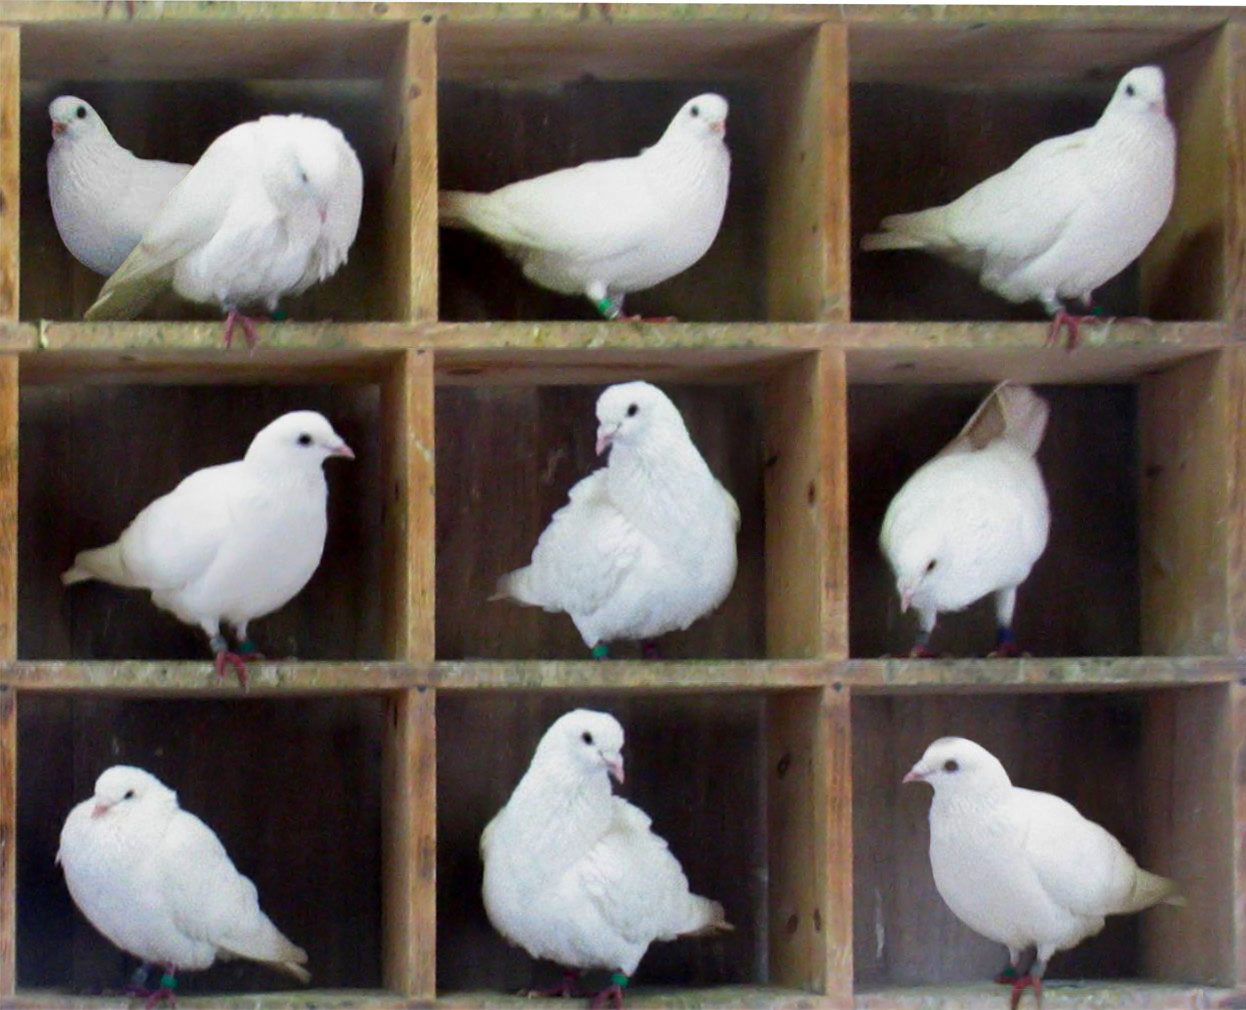
\includegraphics[width=0.4\textwidth]{pics/pigeonhole:TooManyPigeons.jpg}
\end{center}}

The statement sure seems obvious, but let us prove it as a warm-up, and then we'll use it to prove our first claim about birthdays.

\begin{proof}
We use a proof by contradiction.
Assume that none of the boxes has more than one item. Then we would only have at most $k$ items on our hands. But we assumed that the number of items is greater than $k$, so we arrived at a contradiction, and our assumption was false. So there must be a box with at least two items.
\end{proof}


\begin{example}
In a class of 79 students, there are at least two students whose birthdays fall on the same week.
\end{example}

\begin{proof}
Here the weeks in a year -- total of 52 -- play the role of pigeonholes, and students -- total of 79 -- play the role of pigeons.
\end{proof}

\begin{example}
There are two people in Pennsylvania with the same number of hairs on their body.
\end{example}

\begin{proof}
Possible numbers of hairs on a human body play the role of pigeonholes and people play the role of pigeons. By googling, we can find that people usually have 5 million hairs on their body and the population of Pennsylvania is 13 million. Therefore, by pigeonhole principle, there should exist at least two people with the exact same number of hairs.
\end{proof}

Now you may think that that was easy. Let us take it up a notch and see what happens when you have many more pigeons than pigeonholes.

\begin{theorem}[Generalized pigeonhole principle]
\label{thrm:gen_pigeonhole}
If $k>0$ is a number of pigeonholes, and $n$ pigeons try to occupy them, with $n>mk$ for some positive integer $m$, then there will necessarily be a pigeonhole with at least $m+1$ pigeons in it.

In other words, we can say that if $n$ pigeons occupy $k$ pigeonholes, then there is at least one pigeonhole containing at least $\lceil \frac{n}{k} \rceil$ items. The number $\lceil \frac{n}{k} \rceil$ is defined as the smallest integer that is larger than $\frac{n}{k}$.
\end{theorem}

\begin{exercise}
Prove Theorem \ref{thrm:gen_pigeonhole}.
\end{exercise}

\begin{example}
In a class of 79 students, there are at least seven students whose birthdays fall on the same month.
\end{example}

\begin{proof}
Here the months in a year -- total of $k=12$ -- play the role of pigeonholes, and students -- total of $n=79$ -- play the role of pigeons. Then we can calculate that $n = 6 \cdot k + 7$, so by the generalized pigeonhole principle (Theorem \ref{thrm:gen_pigeonhole}) there are at least $6+1 = 7$ students whose birthdays occur in the same month.
\end{proof}

\begin{example}
Pennsylvania needs to have at least two area codes for the phone numbers, while the US needs at least 42.
\end{example}

\begin{proof}
Phone numbers in the US have the format $+1 \, (AAA) \, N******$, where $AAA$ is the area code. The six stars are digits from 0 to 9, while $N$ can only be from 2 to 9. There are more subtle rules that you can find in Wikipedia on the page \href{https://en.wikipedia.org/wiki/North_American_Numbering_Plan#Modern_plan}{``North American numbering plan''}, but further restrictions do not affect the order of magnitude, so let us ignore them for now.
With this, the total possible number of variants to fill the stars is $8 \cdot 10^6 = 8\,000\,000$, so $k=8$ million. As we have found out before, there are $n = 13$ million people in Pennsylvania. So minimal number of area codes is $\lceil \frac{13}{8} \rceil = 2$.

The population of the US is $n=328.2$ million, so you will need at least $\lceil \frac{328.2}{8} \rceil = 42$ area codes.
\end{proof}

In fact, if you google, you will find out that major cities in any state have their own area codes, sometimes a couple, and the total number of area codes is now around 320. 

\begin{exercise}
Can you think of reasons to have so many area codes? (Logistical, social, etc.) Do you think there is a restriction on applying mathematical ideas in real life?
\end{exercise}



%%%
\section{Proving things with the pigeonhole principle}
%%%

Material for this section is take from
\url{https://www.math.uvic.ca/faculty/gmacgill/guide/pigeonhole.pdf}.

As we saw in the above examples, there are four steps involved:
\begin{enumerate}
    \item Decide what pigeons are. They will be the things among which we want to find several of that have the same property.
    \item Set up pigeonholes. In order for the pigeonhole principle to work, it is necessary to have fewer pigeonholes than pigeons. Sometimes you need an astute observation to do this.
    \item Give a rule for assigning the pigeons to the pigeonholes. The pigeonhole principle works for any rule -- you just need to choose the rule that works best for your situation.
    \item Apply the pigeonhole principle to your setup and get the desired conclusion.
\end{enumerate}

\begin{exercise}
Prove that if seven distinct numbers are selected from $\{1, 2,\dots, 11\}$ (braces are used to denote a \emph{set} of objects, e.g. numbers),
then some two of these numbers sum to $12$. Show that you can find six number so that no pair among those sums up to $12$. 
\end{exercise}

\begin{enumerate}
    \item Let the pigeons be the numbers selected.
    \item Let the pigeonholes be labeled by the following sets of numbers: $\{ 1,11 \}$, $\{ 2,10 \}$, $\{ 3,9 \}$, $\{ 4,8 \}$, $\{ 5,7 \}$, $\{ 6 \}$.
    \item The rule: when a number is selected, it is placed in the pigeonhole with the corresponding label.
    \item There are seven numbers and six pigeonholes, so two of the selected numbers will end up in the same pigeonhole. They cannot both end up in the pigeonhole labeled $\{6\}$ because we are choosing distinct numbers, so it's one of the first five. But then they sum up to $12$.
\end{enumerate}

\begin{exercise}
A party is attended by $n \geq 2$ people. Prove that there will always be
two people in attendance who have the same number of friends at the party. (Assume that
the relation ``is a friend of'' is symmetric, that is, if X is a friend of Y then Y is a friend of
X.)
\end{exercise}

Each person either is, or is not, a friend of each of the the other $n-1$ people in
attendance. Thus, the possible values for the number of friends a person can have in
attendance at the party are $0, 1,\cdots,n-1$. However, it can not be the case that there is
someone at the party with $0$ friends and someone else with $n-1$ friends simultaneously: if a person is
friends with everyone, then everyone at the party has
at least one friend there. Thus, the possible values for the number of friends a person can
have in attendance at the party are $0, 1,\cdots,n-2$ or $1, 2,\cdots,n-1$. In either case, there
are $n$ numbers (of friends among the people in attendance) that can take on at most $n-1$
different values. By the Pigeonhole Princple, two of the numbers are equal. Thus, some
two people in attendance who have the same number of friends at the party.

\section{Divisibility}

Let us now make things a little more abstract with numbers.
We will not concern ourselves with where numbers come from 
(although this is a worthy subject in itself)
but will learn how to do things with them.
In particular, we will spend some time thinking about
something that is very closely related to the pigeonhole principle: divisibility.

Let us first equip ourselves with a vocabulary.

\begin{itemize}
    \item \emph{Natural numbers} are numbers that are used for counting, starting
        from 0.
        We denote $\N$ to be the set of all natural numbers.
        Thus, using set notation\footnote{We will discuss sets later.},
        \begin{equation*}
            \N = \set{0,1,2,\dots}\,.
        \end{equation*}
    \item \emph{Integer numbers} are numbers that are used to measure the difference
        between two instances of counting.
        We denote $\Z$ to be the set of all integers.
        Thus, using set notation,
        \begin{equation*}
            \Z = \set{\dots, -2, -1, 0,1,2,\dots}\,.
        \end{equation*}
\end{itemize}

The shorthand of saying ``$a$ belongs to a set $S$ '' is by using the notation
\begin{equation*}
    a\in S \,.
\end{equation*}
For example, the shorthand of ``$a$ is an integer'' is ``$a\in \Z$''\,.

For what to come, we need the notion of the \emph{absolute value} of a number.

\begin{definition}
    The \emph{absolute value} of a number $a$ is a non-negative quantity 
    that represents the size of that number.
    In mathematical terms, 
    \begin{equation*}
        \abs{a} = 
        \begin{dcases}
            a \quad & \text{ if } a \geq 0 \,,  \\
            -a  & \text{ if } a < 0 \,. 
        \end{dcases}
    \end{equation*}
\end{definition}

Our strategy for uncovering the structure of the natural numbers is to break down complex objects and ideas into their fundamental components, think about this quote by Desmond Tutu, a South African Anglican cleric and theologian,
and a human rights activist\footnote{See also \url{https://www.psychologytoday.com/us/blog/mindfully-present-fully-alive/201804/the-only-way-eat-elephant}.}:
\begin{displayquote}
There is only one way to eat an elephant: a bite at a time.
\end{displayquote}
For example, when you prepare for an exam, you make a list of topics and learn one topic at a time; when I prepare lectures, I make a list of topics and write about one topic at a time; in both situations we achieve a complex result by taking many small bites. And when we study natural number, we break them down into their simplest building blocks -- \textit{prime numbers} -- and then study their properties and observe how they interact. One way of breaking the numbers down is to try to divide by a smaller number and observe if there is a remainder. This leads us to the following sequence of definitions.
    
\begin{definition}
    \label{def:divisibility}
    A number $a\in \Z$ is said to be \emph{divisible} by $b\in \Z$ if there exists 
   a number $q\in \Z$ such that 
   \begin{equation*}
       a = bq\,.
   \end{equation*}
   $b$ is called to be a \emph{divisor} (or a \emph{factor}) of $a$ and we can also say that $b$ \emph{divides} $a$ (notation: $b\st a$).

   The number $a$ is \emph{not divisble} by $b$ if $a$ can be written in the form 
   \begin{equation*}
       a = bq +r\,,
   \end{equation*}
   where $q,r \in \Z$ and $0<r<\abs{a}$. The number $r$ is then called the \emph{remainder}.
\end{definition}

    
    Just because I can define something, it doesn't mean that my definition is 
    something that makes sense.
    For example, I can define \emph{a cat} to be a mammal that lays eggs (what's wrong?).
    A good principle in life: question yourself often. Just because
    there are things you can imagine/define, it doesn't mean that those things exist
    or even make sense.

\begin{question}
    Does Definition~\ref{def:divisibility}  make sense? 
    Can there be a number that is both divisible and not divisible by another number?
\end{question}

There is a theorem that guarantees that the situation described in the previous question cannot happen.
In other words, Definition~\ref{def:divisibility} does make sense.

\begin{theorem}[Division theorem]
   Let $a,b \in \Z$ with $b\not= 0$.
   There exist a pair of integers $q,r \in \Z$ such that 
   \begin{equation*}
       a = qb + r \quad \text{ and } \quad 0 \leq r < \abs{b} \,
       ,
   \end{equation*}
   and moreover this pair is unique.
   $q$ is called the \emph{quotient} of $a$ when divided by $b$;
   and $r$ is called the \emph{remainder} of $a$ when divided by $b$.
\end{theorem}

\begin{example}
    Let $a = 101$ and $b = 3$. Then
    \begin{equation*}
        101 = 33\cdot 3 + 2 \,.
    \end{equation*}
    Here, $q =33$ and $r = 2$.
    As said in the division theorem, $2 < 3$.
\end{example}

\begin{example}
   A slightly interesting example is when $ a $ is positive and $b$ is negative.
   Say, $a = 23$ and $b = -4$. Then 
   \begin{equation*}
       23 = (-5) \cdot (-4) + 3 \,.
   \end{equation*}
   In this case $q = -6$ and $r = 3 < 4 $.
\end{example}

We will not prove this theorem for now as it uses the technique of mathematical induction (CS majors would say ``recursion'').

\begin{exercise}
    Read the proof of this theorem in Newstead's book~\cite{Newstead} (Theorem 6.1.1).
\end{exercise}



%%%
\section{Criteria of divisibility}
%%%

Numbers that are divisible by two are called \emph{even}, and they have a special name because in many cultures the distinction between odd and even numbers is quite prominent. For example, ancient Greek and Chinese seem to favor odd numbers like 3 and 5. Russian culture traditionally favors 3 and 7: there is a saying that ``God loves groups of three'', and seven commonly occurs in folk tales. Conversely, Eastern cultures have negative connotations with even numbers, and number 4 in Chinese is associated with death, because quite ominously, we can write it in two ways as an operation on two twos:
$$ 4 = 2\cdot 2= 2+2
.$$
Some buildings in China skip the fourth floor, just like the thirteenth floor is skipped in some places in the US.

On the other hand, Western cultures seem to ``prefer'' even numbers. According to a historian of mathematics (Dr. Nishiyama), ancient preference for odd numbers probably faded in the West with the arrival of modern mathematics as represented by Newton. When counting numbers, odd numbers were incomplete, in-between numbers, whereas even numbers were certainly more ``rational''. This is even reflected in an English proverb that says that two heads are better than one.

So how do we tell even numbers from odd?

\begin{proposition}
An integer number $n$ is divisible by $2$ if and only if its last digit is even (i.e. $0$, $2$, $4$, $6$, $8$).
\end{proposition}

\begin{lemma}
Observe that if a number $a$ is divisible by $b$, then $a + b$, $a + 2b$, etc. are also divisible by $b$. 
\end{lemma}

\begin{proposition}
An integer number $n$ is divisible by $5$ if and only if its last digit is $0$ or $5$.
\end{proposition}


\begin{proposition}
An integer number $n$ is divisible by $4$ if and only if its last two digits comprise a number divisible by $4$. An integer number $n$ is divisible by $8$ if and only if its last three digits comprise a number divisible by $8$. 
\end{proposition}

\begin{proposition}
An integer number $n$ is divisible by $3$ if and only if the sum of all its digits is divisible by $3$.
\end{proposition}

\begin{proof}
Prove the criterion of divisibility by 3 by writing the decimal expansion:
$$ a = a_k \cdot 10^k + \cdots + a_2 \cdot 100 + a_1 \cdot 10 + a_0 \cdot 1
.$$
Notice that $10^k = 9\dots9 + 1$, and the first summand is divisible by 3. So we can write
$$ a - 9\dots9 = a_k + \cdots + a_2 \cdot 100 + a_1 \cdot 10 + a_0 \cdot 1
.$$
Repeat this process and we can see that the right handside would eventually be 
\begin{equation*}
    a_k + \dots + a_1 + a_0 \,.
\end{equation*}
Note that
$a$ and each of the $9\dots 9$ is divisible by 3. Therefore, $a_k + \dots + a_0$ is divisible by 3.
\end{proof}

\begin{proposition}
An integer number $n$ is divisible by $9$ if and only if the sum of all its digits is divisible by $9$.
\end{proposition}

\begin{theorem}
    Let $n>70$ be a natural number that you want to test for being divisible by $7$.
    \\Step 1: Separate the last digit of the number, call it $d$.
    \\Step 2: Double the last digit and subtract from the remaining number, call the result $n_1$:
    $$ n_1 = \frac{(n - d)}{10} - 2 \cdot d
    .$$
    Then $n$ is divisible by $7$ if and only if $n_1$ is divisible by $7$. 
\end{theorem}
If after using this test once, you still get a number $n_1 > 70$, you can repeat the test and get some number $n_2$.

\begin{exercise}
    In 2019, a 12-year old Nigerian boy, Chika Ofili, suggested an alternative test for being divisible by $7$.
    Read the news article about Chika's test: \url{https://www.scilynk.in/divisibility-of-7/}.
    In this test, instead of subtracting $2d$, Chika suggests to add $5d$. What do you think about these two conclusions of the article?
    \begin{itemize}
    \item ``Multiplying by $5$ helps to reach a number within $0$--$70$ at a faster rate compared to multiplication by $2$.''
    \item ``Adding two numbers is psychologically simpler than subtraction.''
    \end{itemize}
    Test these conclusions on some numbers, e.g. 2021, 1234567: count the number of times you apply each test, and try to observe what is easier for you psychologically.
\end{exercise}

%%%
\section{Prime numbers}
%%%

When we factor numbers into smaller numbers, at some point we will have to stop, because there are some natural numbers that cannot be factored as the product of two smaller natural numbers. Trivially, zero and one are among them, but also there are 2, 3, 5, 7, 2017 and 2027.

I would like to argue that zero and one are so special that we don't even call them ``prime''. Most early Greeks did not even consider 1 to be a number, so they could not consider its primality. In modern mathematics, we actually have a formal definition that excludes 0 and 1 as prime numbers.

\begin{definition}
    A natural number $p$ is called prime if it has exactly two positive distinct divisors.
\end{definition}

With this definition, we can observe that 0 and 1 are not prime, because 0 is divisible by any number, while 1 is divisible by only one number -- 1 itself.

\begin{theorem}[Fundamental theorem of arithmetic]
    Every natural number $n>1$ is either a prime or it can be expressed as a product of prime numbers in a unique way.
\end{theorem}

\begin{proof}[Sketch of proof]
We will not prove this theorem because it requires a technique called induction, 
which we have not yet covered.

However, you should be able to see that the existence of such expression is simply 
a matter of definition. If a number cannot be factored into products of smaller number,
by definition, it is a prime number. Keep factoring the smaller number in the products until you get all primes.

The uniqueness part is the tricky part!
\end{proof}

\begin{remark}
   An important idea here is that in mathematics, a proof of unique existence of something
   is often done by two separate steps that are not in any order.
   Existence step is to establish that there is at least one object that satisfies the definition. 
   Uniqueness step is to establish that if two objects with the same definition exist,
   they must be the same.
\end{remark}


\begin{example}
We can first try and factor $2021$. Let's see which prime numbers, starting from the smallest, can divide it: not 2, 3, 5, 7... Eventually, we see that
$$ 2021 = 43 \cdot 47
.$$

Now let us do the same with $2020$. It is divisible by $2$, because its last digit is divisible by $2$:
$$ 2020 = 2 \cdot 1010 = 2^2 \cdot 505 = 2^2 \cdot 5 \cdot 101
.$$
\end{example}

While doing prime decomposition and testing which numbers are prime, you can observe that if $n$ is a natural number that is not divisible by any number up to $\sqrt{n}$, then $n$ is prime.

Sieve method for finding prime numbers.

\begin{theorem}
    There are infinitely many prime numbers.
\end{theorem}
\begin{proof}
    We prove this statement by proof by contradiction. 
    
    Suppose that there are only finitely many primes, listing them as\footnote{
    Note that it is necessary for a finite list of number to have a largest number and a
    smallest number.
    In this case, the largest number in our prime list is $p_n$.
    }
    \begin{equation*}
        p_1 < p_2 < \dots < p_n \,.
    \end{equation*}
    

    Then we claim that the number 
    \begin{equation*}
        a = p_1p_2 \dots p_n + 1 
    \end{equation*}
    is a prime number, which is larger than the largest prime number $p_n$, a contradiction.
    To see that $a$ is a prime number, we suppose that it is not a prime number, then 
    it must be uniquely factorizable by  the primes from $\set{p_1,\dots, p_n}$.
    In particular
    \begin{equation*}
        a = p_{l_1}^{m_1} \cdot \dots \cdot p_{l_k}^{m_k} \,.
    \end{equation*}
    But then we have 
    \begin{equation*}
        1 = p_{l_1}\cdot \dots \cdot p_{l_k} 
        ( p_{l_1}^{m_1-1} \cdot \dots \cdot p_{l_k-1}^{m_k-1} - q ) \,,
    \end{equation*}
    where $q$ is some natural number.
    This is a contradiction because that means both
   \begin{equation*}
       p_{l_1}\cdot \dots \cdot p_{l_k}
   \end{equation*} 
   and 
   \begin{equation*}
       ( p_{l_1}^{m_1-1} \cdot \dots \cdot p_{l_k-1}^{m_k-1} - q )
   \end{equation*}
   must be $1$ or $(-1)$.
   This is impossible as at least
   $ p_{l_1}\cdot \dots \cdot p_{l_k} > 1$ by definition of primes.
\end{proof}

\begin{remark}
   The proof above is by Euclid in 300 B.C.. A remarkable feat! 
\end{remark}

\begin{exercise}
    Infinity is lurking behind us already. You should start asking yourself what
    infinity really is and try to come up with a definition on your own.
\end{exercise}
%%%
\section{Greatest common divisor}
%%%


One of the most fundamental concepts about numbers is the greatest common divisor.

\begin{definition}
    Let $a, b \in \Z$. An integer $d$ is a \emph{greatest common divisor} of $a$ and $b$
    if:
    \begin{enumerate}
        \item $d \st a$ and $d \st b$,
        \item  if $q$ is another integer such that $q\st a$ and $q \st b$ then
            $q \st d$.
    \end{enumerate}
    We denote the (unique) non-negative greatest common divisor of $a$ and $b$ as $\gcd(a,b)$.
\end{definition}

\begin{exercise}
    Why is it that in our definition, we have ``a'' greatest commond divisor, 
    but not ``the'' greatest common divisor?
\end{exercise}

\begin{theorem}
   Let $a,b,q,r \in \Z$ and suppose that $a = qb + r$. Then
   \begin{equation*}
       \gcd(a,b) = \gcd(b,r) \,.
   \end{equation*}
\end{theorem}
\begin{proof}
    First, note that any number $c$ that divides both $a$ and $b$ also divides $r$.
    To see this, we can write $a = m_1 c$ and $b= m_2 c$.
    Therefore, 
    \begin{equation*}
        m_1 c = q m_2 c + r \,,
    \end{equation*}
    which is equivalent to
    \begin{equation*}
        r = c (m_1 - q m_2)\,.
    \end{equation*}
    By definition, $c$ is a divisor of $r$.


    Second, if $d$ divides both $b$ and $r$ then $d$ divides $a$. 
    To see this, we write $b = m_3 d$ and $r = m_4 d$.
    Therefore,
    \begin{equation*}
        a = q m_3 d + m_4 d = (q m_3 + m_4m) d \,.
    \end{equation*}
    
    By those two observations, and definition of greatest common divisor,
    \begin{equation*}
        \gcd(a,b) \leq \gcd(b,r) \quad \text{ and } 
        \quad \gcd(a,b) \geq \gcd(b,r) \,.
    \end{equation*}
    This means that 
   \begin{equation*}
       \gcd(a,b) = \gcd(b,r) \,,
   \end{equation*}
   as desired.
\end{proof}



One question arise, how can we find the greatest common divisor of any two numbers?
For example, how on earth are we supposed to know $\gcd(199888,4987774)$?
Luckily, ancient people were pretty smart and there is a method that was invented
at least 2300 years ago as it first appeared in Euclid's Elements (300 BC).
We, as modern people, still benefit from this method as it has a lot of practical applications~\footnote{For a curious mind, you can read more about it here: \url{https://en.wikipedia.org/wiki/Euclidean_algorithm}}.

\begin{theorem}[Euclid's algorithm]
    Let $a,b \in \Z$. The $\gcd(a,b)$ is computed as follows.
    \begin{itemize}
        \item Set $r_1$ to be the remainder of $a$ divided by $b$ .
        \item Set $r_2$ to be the remainder of $b$ divided by $r_2$.
        \item Given $r_{n-2}$ and $r_{n-1}$, define $r_n$ to be 
            the remainder of $r_{n-2}$ divided by $r_{n-1}$.
        \item Stop when $r_{n+1} = 0$; then $r_{n} = gcd(a,b)$.
    \end{itemize}
\end{theorem}
Writing everything explicitly, we have
   \begin{gather*}
       a = bq_1 + r_1 \qquad ( 0< r_1 < b)\\ 
       b = r_1q_2 + r_2 \qquad ( 0< r_2 < r_1)\\ 
       r_1 = r_2 q_3 + r_3 \qquad ( 0< r_3 < r_2) \\
       \dots \\
       r_{n-2} = r_{n-1} q_{n} + r_n \qquad ( 0< r_n < r_{n-1}) \\
       r_{n-1} = r_n q_{n+1} + 0  \,.
   \end{gather*}
Then $\gcd(a,b) = r_n$.

\begin{exercise}
   Why must there is a $0$ remainder at the end of Euclid's algorithm?
   This is an important question because it answer the following question,
   ``why should the algorithm stop?''
   Is there a scenario when you have to do this forever?
\end{exercise}

\begin{example}
   Use Euclid's algorithm to find
   \begin{equation*}
       \gcd(242, 66)\,.
   \end{equation*}
    Let's compute!
    \begin{gather*}
       242 = 66\cdot 3 + 44\\
       66 = 44\cdot 1 + 22\\
       44 = 22\cdot 1 + 0\,.
    \end{gather*}
    So $\gcd(242,66) = 22$.
\end{example}


Let's have some fun with greatest common divisors using Euclid's algorithm.
\begin{corollary}
    Let $l = \gcd(a,b)$. Then there exist two integers $m,n$ such that
    \begin{equation*}
        l = am + bn\,.
    \end{equation*}
\end{corollary}
\begin{proof}
   We apply Euclid's algorithm to prove this statement. 
   Writing everything explicitly, we have
   \begin{gather*}
       a = bq_1 + r_1 \qquad ( 0< r_1 < b)\\ 
       b = r_1q_2 + r_2 \qquad ( 0< r_2 < r_1)\\ 
       r_1 = r_2 q_3 + r_3 \qquad ( 0< r_3 < r_2) \\
       \dots \\
       r_{n-2} = r_{n-1} q_{n} + r_n \qquad ( 0< r_n < r_{n-1}) \\
       r_{n-1} = r_n q_{n+1} + 0  \,.
   \end{gather*}
   We know that, $l = r_n$ because that is the content of Euclid's algorithm.

   Now, to show what we want to show, we reverse engineer what's happening.
    Rewriting 
    \begin{equation*}
        r_1 = a - bq_1\,.
    \end{equation*}
    Then,
    \begin{equation*}
        r_2 = b - r_1 q_2 = b - (a + b q_1)q_2 = (1 - q_1q_2) b - q_2 a \,.
    \end{equation*}
    Keep doing this until $r_n$ and we will arrive at our conclusion.
\end{proof}


\chapter{Logic}



At its core, mathematics is a way of reasoning and is very similar to philosphy.
The first part of this chapter wil reflect this basic observation.
However, what sets apart mathematics from general philosophy is that 
the language of mathematics requires precision. 
There should be no ambiguity in a mathematical statement.
%This is a blessing as well as a curse because the cost of being pricise
%is to be terse and, sometimes, aesthetically unpleasant.
%However, as for a lot of things in life, hidden beneath its scary-looking
%appearance is a wealth of beautiful treasures that are the rewards for those
%who steadfastly endure until the end.
The main goal of this chapter 
is to give the students a taste of what it is like to be mathematically
precise.

%%%
\section{What can logic be about?}
%%%
We follow~\cite{Sainsbury1991} for this part.

Most broadly, logic is about reasons and reasoning. There are reasons for
\textit{acting}: you may avoid sugary desserts for the reason of wanting to keep thin or lose weight. There are reasons for 
\textit{believing}: you may think that the potatoes are ready to eat for the reason that they have been boiling for twenty minutes. 
Historically, logic has concerned itself with reasons for believing. 
But even this question can be answered in various ways. For example, I asked an Indian friend of mine why she believes that she should not eat meat. Her answer was that this belief was instilled in her by her family at an early age. This explains the origin of this belief, but does not give a \emph{reason} for it. But then she continued her answer and said that now she doesn't like the smell of meat, and eating food that smells bad is usually a bad idea. This also justifies her belief. Some other people may say that killing anything is wrong, and eating meat requires killing, thus reasoning why they shouldn't eat meat. 

The way it works is that one deduces the reasons for a certain belief by
making it a consequence of a ``higher'', more abstract, belief.
Logic as a discipline of ``good reasoning'' was first considered as early as the 6th century B.C. and independently in India, Greek and China.

\begin{example}
    Consider the following chain of sentences.

    ``I believe that humans breath oxygen to live. I believe that I am a human.
    Therefore, I believe that I breath oxygen to live.''

    ``All humans breath oxygen'' is a higher, more abstract, fact than `` I breath
    oxygen'', as I am just a particular member of the human race.
\end{example}

\begin{warning}
   Not every belief has its reasons. Every logical system has its core ``beliefs''
   (called \emph{axioms})
   that are taken for granted,
   and they have no further explanation.
   These are the most abstract beliefs that are used to deduce every other belief in
   the same logical system.
   To have reasons, one needs to take a leap of faith at some point.
\end{warning}


Logic is a \emph{normative} discipline.
It sets out standard for \emph{good} and \emph{bad} arguments.
These are technical terms and should not be confused by subjective opinions.
However, the these technical terms are somewhat inspired by daily
commonsense distinction between good and bad reasons.
In our daily conversation, to make good reasons for something is to create 
premises so that the something \emph{follows}.

\begin{example}
    ``James is a banker and all bankers are rich'' is a good reason for
    ``James is rich.''
\end{example}

\begin{question}
    If James is not a banker, can we conclude that he is not rich?
\end{question}

\begin{example}
    ``James likes expensive cars'' is not a good reason for ``James is rich.''
\end{example}


It is important to note that one can discern good and bad reasons without having to
believe in the reasons themselves.
In fact, Einstein himself did not believe in (even reject) 
quantum physics while being one of the 
founding fathers of the theory.
A lot of modern mathematics revolves around physics and biology but a lot of mathematicians barely know any physics or biology (confession time).

    
\subsection{Inductive and deductive logic}
The result of assembling premises and conclusions together is called an \emph{argument}.
An argument is \emph{valid}, or \emph{true}, or \emph{good}, if the conclusions follow from the premises.
The two most common forms of logic are inductive logic and deductive logic.

An example of inductive logic is the following.
\begin{example}
    The sun has risen every morning so far; therefore it (probably) will rise tomorrow.
\end{example}

\begin{exercise}
    Contrast the previous example with the following sentence:

    `` The sun has risen every morning so far; therefore it (probably) will NOT rise tomorrow.''

   Is one of these sentences more true than the other? How do you know?
\end{exercise}

An example of deductive logic is the following.
\begin{example}
   All men are mortal. Socrates is a man. Therefore, Socrates is mortal. 
\end{example}

Thus, a way to distinguish between inductive and deductive logic is:
for deductive logic, it is impossible for the conclusion to be false if the premises are true.
For inductive logic, this is not the case as the conclusion in this case may be false
despite the premises being true.
We can see that it is only in deductive logic, one can talk about the validity of an argument.
In inductive logic, there are degrees in strength of an argument but inductive reasoning 
can \emph{never be valid} by our definition of validity\footnote{Be careful here that
    validity is a technical term and should not be confused with the daily use of 
the word}.
However, an inductive argument can be stronger than another inductive argument 
(just make sure one is talking about the same thing -- comparing apples to apples and not to pears).

Mathematics is all about deductive logic whereas science must involve both inductive
and deductive logic.
The combination of inductive and deductive logic in science gives birth to the need of probability and
statistics (whose theories are all mathematical and deductive), and in modern day data science and machine learning that are based on statistics.

\begin{warning}
   Do not confuse inductive logic with the method of induction, which is a method
   in deductive logic.
   Although, there are resemblance between the two. The difference is that in the method
   of induction,
   one is given the super power in theory to transcend time to ``go off to infinity''
   whereas inductive logic is limited by physical evidence, where 
   time is a major road block...
\end{warning}

\begin{exercise}
    Make a table of comparison between inductive and deductive logic.
\end{exercise}

Watch this lecture about inductive logic: \url{https://youtu.be/DRx-3jvC918}.

\begin{exercise}
   What's wrong with the following?
    
   Statement: You have horns.
   
    "Proof": What you haven't lost, you have. You haven't lost your horns. Therefore you have horns. 
\end{exercise}

\begin{exercise}
   What's wrong with the following?
    
   Statement: You don't know your father.

    "Proof": I show you a photo of someone, the photo is covered by a cloth. Do you know who's in the photo? You can't see, so you don't. But it's a photo of your father. Therefore you don't know your father.
\end{exercise}

%%%
\section{Mathematical logic}
%%%
We follow~\cite{Newstead} for this part.

Mathematical logic is the study of logic restricted to mathematics. 
Its existence is to address the biggest problem in the foundation of mathematics: 
are theories of mathematics consistent with each others?
That said, many working mathematicians do not pay attention to the question of foundations, which might be a worrisome fact.
I can only have my fingers crossed that mathematics will not fall apart one day 
(which, it did for a period of time, when Georg Cantor discovered different infinities in the 19th century)...

A {\bf mathematical statement} is a statement that  
at least the statement maker has to be able
to assign a {\bf truth value} (`true' or `false') to it.
The truth assignment could be the result of an immediate observation or
a long chain of difficult reasoning.
To make the truth assignment valid, every single argument in the chain of reasoning
must be valid.
A {\bf proof} of a mathematical statement is a chain of valid arguments that make
the mathematical statement \emph{true}.
\murmuno{?}
\SV[Aug 13]{ fixed- thanks}
%with others.

There are many names for a \emph{true} mathematical statement, depending on the use:
\begin{itemize}
    \item {\bf Theorem:} a particularly important mathematical statement 
        given the context.
    \item {\bf Proposition:} general term that can be used anytime.
    \item {\bf Lemma:} a mathematical statement that will be used as a stepping
        stone to prove a theorem.
    \item {\bf Corollary:} a mathematical statement whose truth value could be deduced
        from a theorem without much effort.
\end{itemize}

A statement that are believed to be verifiable but no human has seen or 
discovered its proof yet is called a {\bf conjecture}.

\subsection{Structure}
Every mathematical statement has the following structure:

\begin{center}
    Assumptions + Goals
\end{center}

\begin{example}
    Suppose Philadelphia is in Massachusetts and Penn is in Philadelphia, then Penn is in Massachusetts.
\end{example}

\begin{warning}
    Assumptions themselves need not to be true. 
    We will talk more about this later when we talk about truth table.
\end{warning}

\begin{exercise}
    Find an example of a famous mathematical statement  that its assumptions are not yet verified.
\end{exercise}
\murmuno{What are your examples?}
\SV[aug 13]{I have one example about the hypothesis that particles in a room behave as if they are independent identically distributed. This is the key assumption to derive the Boltzmann equation.
Something that stem from Riemann hypothesis?}

\begin{example}
    For example, abc conjecture implies Fermat's last theorem. But as of now, the status of the abc conjecture is subject to debate. A Fields medalist Peter Scholze and Jakob Stix found a gap in Mochizuki's proof.
    
    Now a quote from Wikipedia: ``Scholze and Stix wrote a report asserting and explaining an error in the logic of the proof and claiming that the resulting gap was ``so severe that ... small modifications will not rescue the proof strategy''; Mochizuki claimed that they misunderstood vital aspects of the theory and made invalid simplifications.

    On April 3, 2020, two Japanese mathematicians announced that Mochizuki's claimed proof would be published in Publications of the Research Institute for Mathematical Sciences (RIMS), a journal of which Mochizuki is chief editor. In March 2021, Mochizuki's proof was published in RIMS.''
\end{example}

We will end this section by discussing a few logical axioms that look obvious
but people use all the time in mathematics without realizing it.

   

\section{Symbolic logic}
One of the main goals of mathematics is to reduce complicated statements/observations
to simple abstract structures that are more tractable to human minds and still
keep the essential features of the things one would like to study.
This is as much of an art as anything else because too much abstraction would
lead to triviality, which may not be very interesting.

{\bf Symbolic logic} is a system of logic that can be used to reduce a mathematical 
statement into ``agreed'' formulas that are easier to determine its truth 
value.\footnote{
    Gottfried Leibniz (another inventor of Calculus) was among 
    the first people to realize the importance of having a system
of logic that is universal and calculatable but couldn't actualize this dream.
The goal was to reduce confusions and disputes among philosophers and arguers.
(Just turn on the Presidential debates and you will understand why we need
such a system...)
The first well-known work that successfully made symbolic logic a mathematical field
was by George Boole in 1854~\cite{Boole2009}.
One of the earliest work that started the 
modern account of logic and foundation of mathematics was by Russel and 
Whitehead~\cite{WhiteheadRussell1997} 
(there is a comic book about it~\cite{DoxiadisPapadimitriou2009}!).
}

Let us consider a simple example from~\cite{Newstead}:
\begin{example}
    \label{ex:divides}
    If $c$ divides $b$ and $b$ divides $a$, then $c$ divides $a$.
\end{example}

We see that each of the statements ``$c$ divides $b$'', ``$b$ divides $a$'',
and ``$c$ divides $a$'' is a proposition if they stand alone by themselves.
Thus, abstractly, each of them could be assigned a symbol 
    \begin{itemize}
        \item $P =$ $c$ divides $b$
        \item $Q = $ $b$ divides $a$ 
        \item $R = $ $c$ divides $a$ 
    \end{itemize}

Then you can write
\begin{center}
    If $P$ and $Q$, then $R$.
\end{center}
The above form of the statement looks easier to follow (at least to the 
mind of a non-English speaker) since at least 
we don't need to know what ``divides'' means.
While it is not too useful in terms of conveying knowledge, it is 
extremely useful when it comes to determining the validity of the statement itself.
This leads us to the next question: \emph{What makes a statement true?}

We will need a few new words.

\begin{definition}
    A {\bf propositional variable} is a symbol that represents a proposition.
\end{definition}
As we said earlier, propositions are just mathematical statements, which are
required to have truth values (`true' or `false').

\begin{definition}
    A {\bf logical operator} is a symbol (or collection of words) that turn 
    one or more propositional variables to a \emph{single} new statement.
\end{definition}

Basic logical operators are:
\begin{itemize}
    \item Conjuction (`and', $\wedge$)
    \item Disjunction (`or', $\vee$)
    \item Implication (`if...then...', $\implies$)
    \item Negation (`not', $\neg$)
\end{itemize}
As simple as they look, these four operators build most of  mathematics
and anything that require reasoning (philosophy, law, computer science, etc.).



\begin{definition}
    A {\bf propositional formula} is an expression that is either a propositional 
    variable, or is built up from simpler propositional formulae using logical
    operators.
\end{definition}
\begin{remark}
    When I ask, ``What is the variable for the proposition?'', I am more
    interested in what the symbol you give to the mathematical statement, not
    so much the content of it.
    Similarly, when I ask, ``What is the formula for the proposition?''
    I am more interested in the way the proposition is written up, not so much
    what the proposition conveys.
\end{remark}
    
The simplest kind of propositions is one that only contains one single 
propositional variable that already explicitly has the truth value  (`true' or `false')
known (whether it is a \emph{proven statement}, \sout{a common knowledge} or an assumption).
\SV[2021-08-17]{I emphasize that common knowledge may not be trusted always}
\murmuno[08-26]{We can ask to give examples of ``common knowledge'' about some topic, e.g. time (less divisive), and find contradictions. * Time is money. * Life is a marathon, not a sprint. * The two most powerful warriors are patience and time. * Time waits for no one. * Better three hours too soon than a minute too late. * The key is in not spending time, but in investing it. * Punctuality is the thief of time. }
From these atomic propositions, we could build more complicated kinds of propositions
with more complicated propositional formula
by obeying certain logical rules of the logical operators\footnote{Even though we call them rules, they follow an
    intuitive model of our daily reasoning. 
    The advantage of defining explicit rules is to make the 
    reasoning more consistent by the abstraction.}.
    This process is  entirely ``calculatable''.
\SV[08-28]{Agreed.}
Here are the rules for the basic logical operators listed above.

{\bf Conjunction (`and', $\wedge$).}
 The propositional formula for a proposition made by a conjuction has the following form
\begin{equation*}
    P \wedge Q \,.
\end{equation*}
\begin{rule*}
The proposition $P \wedge Q$ (we say ``$P$ and $Q$'') is true if {\bf both} $P$ and $Q$ are true.
Otherwise, if either (or both) $P$ or $Q$ is false, $P \wedge Q$ is false.
\end{rule*}

{\bf Disjunction (`or', $\vee$).}
 The propositional formula for a proposition made by a disjunction has the following form
\begin{equation*}
    P \vee Q \,.
\end{equation*}
\begin{rule*}
    The proposition $P \vee Q$ (we say ``$P$ or $Q$'') is true if { \bf either one} 
    (or both) of $P$ or $Q$ is true.
    $P \vee Q$ is flase if {\bf both} $P$ and $Q$ are false.
\end{rule*}

{\bf Implication (`if...then...', $\implies$).}
 The propositional formula for a proposition made by a disjunction has the following form
\begin{equation*}
    P \implies Q \,.
\end{equation*}
\begin{rule*}
    The proposition $P\implies Q$ (we say ``$P$ implies $Q$'') is true if one of
    the following cases holds:
    \begin{itemize}
        \item $P$ is true and $Q$ is true.
        \item $P$ is false.
    \end{itemize}
\end{rule*}

\begin{exercise}
   This is one of the most confusing rules in logic. 
   Meditate on the rule of implication. 
\end{exercise}


{\bf Negation (`not', $\neg$).}
 The propositional formula for a proposition made by a disjunction has the following form
\begin{equation*}
    \neg P \,.
\end{equation*}
\begin{rule*}
    The proposition $\neg P$ (we say ``not $P$'') is true if $P$ is false.
\end{rule*}



\begin{exercise}
    Mess with your friends/parents/siblings with `and', `or', `if not ... then...'
\end{exercise}

\begin{axiom}[Law of excluded middle]
   Let $P$ be a propositional formula. 
        Then $P \vee (\neg P)$ is true.
        In plain English, this says that every proposition is either true or false.
\end{axiom}

\begin{axiom}[Principle of explosion]
     If a contradiction is assumed, any consequence may be derived.  
\end{axiom}
 
 
\section{Variables and quantifiers}

\subsection{Variables}

It is nice to know basic rules of logic and how propositions work in sequences
in order to produce proofs (arguments).
It is unfortunate, however, that if we only work with propositions, our reasoning would 
be fairly limited.
Consider the following sentence:
\begin{center}
   ``$x$ is divisible by $7$.''
\end{center}

\begin{question}
    Is this a proposition?
\end{question}
\begin{proof}[Answer]
   This is not a proposition as one cannot assign a truth value to it-- 
   we don't know what $x$ is.
\end{proof}


\murmuno[08-26]{We can include a topic on most common logical fallacies and advertise blog LessWrong and the long fanfic ``Harry Potter and the Methods of Rationality''.}

\SV[08-28]{That sounds like fun.}

If we know a specific value of $x$, we would be able to determine the truth value
of the sentence above and it would become a proper proposition. For example, if $x = 49$,
the sentence would be true and if $x = 42$, it would be false.
If we suppose that $x$ should belong the set of natural number, $\N$, 
then The symbol $x$ is called a \emph{free variable}
the set $\N$.

\begin{definition}
    Let $x$ be a variable that is understood to refer to an element of a set $X$. 
    In a statement involving $x$, we say it is \emph{free} if it makes sense to
    substitute particular elements of $X$ in the sentence; otherwise we
    say $x$ is \emph{bound}.
\end{definition}

So if the sentence in the above question is not a proposition, what do we call it?
Glad you ask-- statements like those, which depend on free variables (hence abstract
the notion of proposition) are called \emph{predicate}.
More formally, we have the following definition.

\begin{definition}
    A \emph{predicate} is a symbol $P$ with a specified list of free variables $x_1, x_2, \dots, x_n$ and, for each variable $x_i$, a specification of a set $X_i$ (called the \emph{domain of disclosure} of $x_i$).

    Notation: we will typically write $P(x_1,\dots, x_n)$ in order to make the variable
    explicit.
\end{definition}

\begin{example}
    We can represent the sentence `$x$ is divisible by $7$' by $P(x)$, where $x \in \N$.
    $P(49)$ is true and $P(10)$ is false.
\end{example}

\begin{example}
    \label{e:exists}
   The sentence ``there exist integers $a,b$ such that $x = a^2 + b^2$'' has free
   variable $x$ and bound variables $a^2+ b^2$, 
   and can be represented by a predicate $R(x)$, where the domain of disclosure 
   can be chosen to be $\Z$.
\end{example}

\begin{remark}
    A predicate with no free variables is precisely a propositional variable.
\end{remark}

\begin{exercise}
    How would you represent the sentence ``$x-y$ is rational'' as a predicate.
\end{exercise}

\begin{exercise}
    \label{e:every}
    How would you represent the sentence ``every even natural number $n\geq 2$ is
    divisible by $k$''?
\end{exercise}


\subsection{Quantifiers}
Looking back to Example~\ref{e:exists} and Exercise~\ref{e:every}, we notice that
the bound variables come with either ``there exist'' or ``every''.
Without those terms, those variables will be come free variables.

Expressions that refer to \emph{how many} elements of a set make a statement true,
such as ``there exists'' and ``every'' turn free variables into bound variables.
We represent such expression using symbols called \emph{quantifiers}.

In mathematics, there are two \emph{universal quantifiers}, 
$\forall$ (every) and $\exists$ (there exists).

\begin{example}
    intuitively speaking,
   \begin{itemize}
       \item The expression ``$\exists x \in X$'' denotes ``there exists $x\in X$''.
        \item The expression ``$\forall x\in X$'' denotes ``for every $x\in X$''.
   \end{itemize} 
\end{example}

Just like we can build propositional formulae from propositions and logical operators, 
we can build something out of predicates and logical operators.
\begin{definition}[{\bf Logical formula}]
    A \emph{logical formula} is an expression that is built from predicates using logical
    operators and quantifiers; it may have both free and boundary variables.
    The truth value of a logical formula depends on the free variables according 
    to the rules for logical operators and quantifiers.
\end{definition}
It is an important skill to translate from human languages into purely symbolic logical formulae
and vice versa.

Formally, we have the following definitions of quantifiers.

\begin{definition}[\bf The universal quantifier $\forall$]
    If $p(x)$ is a logical formula with free variable with free variable $x$ with domain $X$,
    then $\forall x\in X, p(x)$ is the logical formula defined according to the following rules:
    \begin{itemize}
        \item If $p(x)$ can be derrived from the assumption that $x$ is an arbitrary element of $X$,
            then $\forall x\in X, p(x)$;
        \item If $a\in X$ and  $\forall x \in X, p(x)$ is true, then $p(a)$ is true.
    \end{itemize}
\end{definition}

\begin{definition}[\bf The universal quantifier $\exists$]
    If $p(x)$ is a logical formula with free variable $x$ with domain $X$, then 
    $\exists x\in X, p(x)$ is the logical formula defined according to the following rules:
    \begin{itemize}
        \item If $a\in X$ and $p(a)$ is true, then $\exists x \in X, p(x)$;
        \item If $\exists x\in X, p(x)$ is true, and $q$ can be derived from the assumption
            that $p(a)$ is true for some fixed $a \in X$, then $q$ is true.
    \end{itemize}
\end{definition}

There are more quantifiers out there in the wild world of mathematics but they depend
on specific fields of study. The above two quantifiers are used in every field of mathemtics, however.

One can combine quantifiers in a logical formula and the order of the quantifiers matter.
\begin{exercise}
   Translate the following expressions and convince yourself that they are different. 
   \begin{enumerate}
       \item $\forall x \in \Z, \exists y \in \Z, \exists z \in \Z, x = y^2 + z^2$. 
       \item $\exists y \in \Z, \exists z \in \Z, \forall x \in \Z, x = y^2 + z^2$. 
       \item $\exists y \in \Z, \forall x \in \Z,\exists z \in \Z,  x = y^2 + z^2$. 
   \end{enumerate}
   Are those propositions?

   Are the following statements different?
    \begin{enumerate}
       \item $\forall x \in \Z, \exists y \in \Z, \exists z \in \Z, x = y^2 + z^2$.
       \item $\forall x \in \Z, \exists z \in \Z, \exists y \in \Z, x = y^2 + z^2$. 
   \end{enumerate}
\end{exercise}


\subsection{Logical equivalence}

We start out with a question
\begin{question}
    Let $P$ be the set of all prime numbers.
   Are these two logical formulae the same?
   \begin{enumerate}
       \item $\forall n \in P, (n> 2 \implies (\exists k \in \Z, n = 2k+ 1))$.
       \item $\neg \exists n \in P, (n> 2 \wedge ( \exists k \in \Z, n = 2k))$.
   \end{enumerate}
\end{question}
In plain English, the two logical formulae read as follows.
\begin{enumerate}
    \item Every prime number greater than two is odd.
    \item There does not exists an even prime number greater than two.
\end{enumerate}

Because of the way they are framed, one would go on  to prove these statements
by using two completely different techniques.
\begin{enumerate}
    \item Fix a prime number $n$, assume that $n>2$, and then prove that $n = 2k+ 1$
        for some $k\in \Z$.
    \item Assume that there is some prime number $n$ such that $n>2$ and $n=2k$ for some
        $k \in \Z$ and derive a contradiction.
\end{enumerate}
\begin{question}
   Which strategy is easier to follow/prove?
\end{question}

One can see that knowing more ways to rephrase a statement gives us more ways to
prove/disprove it.
The notion of \emph{logical equivalence} tells us exactly when two statements 
have the same logical meaning, hence gives us confidence to think about one
statement in the form of a different statement
without worrying about being led astray by irrelevant thoughts and discover
later that all the work we have done was in vain (even though this happens all the time).

\begin{definition}
    Let $P$ and $Q$ be logical formulae.
    We say that $P$ and $Q$ are logically equivalent and write $P\equiv Q$
    if $Q$ can be derived from $P$ and $P$ can be derived from $Q$.
\end{definition}

\begin{example}
    \label{ex:equiv1}
   We claim that
   \begin{equation*}
       P \wedge (Q \vee R) \equiv (P \wedge Q) \vee (P \wedge R) \,,
   \end{equation*}
   where $P, Q, R$ are propositional variables.

   \begin{proof}
       First, assume that $P \wedge (Q \vee R)$ is true. 
       Then $P$ is true and $Q\vee R$ is true by definition of conjunction.
       By definition of disjunction, either $Q$ is true or $R$ is true. So, we divide
       our reasoning into two cases:
       \begin{itemize}
           \item If $Q$ is true, then $P \wedge Q$ is true by definition of conjunction.
           \item If $R$ is true, then $P \wedge R$ is true by definition of conjunction.
       \end{itemize}
       In both cases, we have that $(P \wedge Q) \vee (P \wedge R)$ is true by
       definition of disjunction.

       Second,
       assume that $(P \wedge Q) \vee (P \wedge R) $ is true.
       Then, either $P \wedge Q$ is true or $P \wedge R$ is true by definition of disjunction.
       Again, we divide our reasoning into two cases:
       \begin{itemize}
           \item If $P \wedge Q$ is true, then $P$ is true and $Q$ is true by definition of conjunction.
           \item If $P \wedge R$ is true, then $P$ is true and $R$ is true by definition of conjunction.
       \end{itemize}
       In both cases, we have $P$ is true and $Q \vee R$ is true by definition of disjunction.
       Therefore,
        $P \wedge (Q \vee R)$ is true.

        Thus, we have derived that $(P \wedge Q) \vee (P \wedge R)$ is true from 
        $P \wedge (Q \vee R)$ being true and vice versa.
        This proves our claim by definition of logical equivalence.
   \end{proof}
   
\end{example}

Now we turn to everyone's favorite tool, the \emph{truth table}.

\subsection{Truth table}

\begin{definition}
    The truth table of a propositional formula is the table with one row for each 
    possible assignment of truth values to its constituent propositional variables, 
    and one column for each sub-formula 
    (incluidng the propositional variables and the propositional formula itself).
    The entries of the truth table are the truth values of the 
    sub-formulae.
\end{definition}

There are many ways that one could employ to prove the logical equivalences
of propositional formulae. 
The most fundamental way is to use the definition.
Another way that is one of the all-time favorites is to use the truth table: 
in order to prove that propositional formulae are logically equivalent, 
it suffices to show that they have identical columns in a truth table.

\begin{example}
    We will prove the what's claimed in Example~\ref{ex:equiv1} using the truth table. 
\end{example}

\begin{center}
\begin{tabular}{ |c|c|c|c|c||c|c|c| } 
\hline
P & Q & R & $Q \vee R$ & $P \wedge (Q \vee R)$ & $P \wedge Q$ & $Q \wedge R$ & $(P\wedge Q) \vee (P \wedge R)$ \\
\hline
T& T & T &T & T & T & T & T\\ 
T& T & F & T & T & T & F & T\\ 
T& F & T & T & T & F & T & T\\ 
T & F & F & F & F &F & F &F \\
F & T& T & T & F&F & F &F\\
F & T& F & T & F&F & F &F\\
F & F& T &T & F&F & F &F\\
F & F& F & F & F&F & F &F\\ 
\hline
\end{tabular}
\end{center}

\begin{example}
   Use the truth table to show that
   \begin{equation*}
       P \implies Q \equiv (\neg\, P) \vee Q\,.
   \end{equation*}
\end{example}

\begin{theorem}[De Morgan's laws for logical operators]
   Let $P, Q$ be propositional variables. Then,
   \begin{enumerate}
       \item $\neg (P \vee Q) \equiv (\neg P) \wedge (\neg Q) $,
       \item $\neg (P \wedge Q) \equiv (\neg P) \vee (\neg Q) $ .
   \end{enumerate}
\end{theorem}

\begin{theorem}[De Morgan's laws for quantifiers]
    Let $P(x)$ be a logical predicate and $X$ be a set. Then,
   \begin{enumerate}
       \item $\neg (\forall x \in X, P(x) ) \equiv \exists x\in X, \neg P(x) $,
       \item $\neg (\exists x \in X, P(x)) \equiv \forall x\in X, \neg P(x) $ .
   \end{enumerate}
\end{theorem}

\chapter{Sets and functions}
\section{Sets}

The notion of a \emph{set} is extremely fundamental (as we already used it in 
previous discussions) yet, if not defined carefully, could lead to paradoxes and
break mathematics from its core.
Perhaps the most infamous paradox in naive set theory  is the so-call Russell's paradox.
However, for the sake of sanity in this course, let's stick with the naive notion 
and trust that mathematicians already fixed this issue and unbroke mathematics...
\begin{definition}
   A set is a collection of objects. 
   The objects in the sets are called \emph{elements} of the set.
   If $x$ is an element in the set $X$ then we write $x\in X$.
   We write $x\not\in X$ to mean $\neg (x\in X)$.
\end{definition}

The way that Bertrand Russell broke naive set theory is via the following chain of reasoning, taken directly from Wikipedia:

\begin{displayquote}
   Let $R$ be the set of all sets that are not members of themselves.
   If $R$ is not a member of itself, then its definition entails that 
   it is a member of itself; if it is a member of itself, 
   then it is not a member of itself, since it is the set of 
   all sets that are not members of themselves. 
\end{displayquote}

We will need to use the so-called \emph{set-builder notation} to
describe sets in general.
Given a set $X$, set set of elements of $X$ satisfying some property $P(x)$ is denoted by
\begin{equation*}
\set[\big]{ x \in X \st P(x)} \,.
\end{equation*}


From now on, we define the set of all rationals to be 
\begin{equation*}
    \Q = \set[\big]{ p / q \st p \in \Z, q\in \Z \text{ and } q\not= 0} \,,
\end{equation*}
and the set of real numbers to be
\begin{equation*}
\R = \set[\big]{ \text{rationals and irrational numbers}}\,.
\end{equation*}
We are cheating in the definition of real numbers above but that is too technical for the moment. Let's just go with what you imagine it to be from high school.
We will also use the usual open and closed set notations.
\begin{gather*}
[a,b] = \set[\big]{x \in \R \st a \leq x \leq b } \,,\\
[a,b) = \set[\big]{x \in \R \st a \leq x <  b } \,, \\
(a,b] = \set[\big]{x \in \R \st a < x \leq  b } \,, \\
(a,b) = \set[\big]{x \in \R \st a < x <  b } \,.
\end{gather*}

See Newstead~\cite{Newstead} (Chapter 2) for representations of intervals on the number line.

\begin{definition}
    Let $X$ be a set. A \emph{subset} of $X$ is a set $U$ such that 
    \begin{equation*}
        \forall a, ( a \in U \implies a \in X) \,.
    \end{equation*}
    We write $U \subseteq X$ for the assertion that $U$ is a subset of $X$.
    The notation $\subsetneqq$ means that $U$ is a \emph{proper subset} of $X$, 
    that is a subset of $X$ that is not equal to $X$.
\end{definition}

In order to prove that $U$ is a subset of $X$, it is sufficient to take an 
arbitrary element $a\in U$ and prove that $a \in X$.

\begin{example}
    Prove that $\Z \subset \Q$.
\end{example}

We want to be able to say when two sets are the same (equal) with each other.
There are different ways to go about this.
One can say that two sets are equal if they have the exact same definition or
there definition are somehow logically equivalent to each other.
In real practice, these are not very useful.
However, there are those who believe that ``we are what we are made of.''
This sounds like a reasonable description and is a criteria to distinguish two different
people. Surely, even though our bodies might be made of atoms
but my atoms are different than your atoms.
This inspires the following axiom about set equality.


\begin{axiom}[Axiom of extentionality]
   Let $X$ and $Y$ be sets. Then $X = Y$ if and only if $X \subseteq Y$ and $Y\subseteq X$. 
\end{axiom}

\begin{example}
   Prove that, 
   \begin{equation*}
   \set[\big]{ x \in \R \st x^2 \leq 1 } = [-1,1] \,.
   \end{equation*}
\end{example}

One question may arise when we define intevals.
Consider, $(a,b)$, for example. Some people might object this definition because
if $a >b$ we have a contradiction 
\begin{equation*}
    b< a < x < b \,.
\end{equation*}
How can this be?
A careful look at this definition, we realized that it says, 
if $x \in \R$ and $ a< x <b$, then we admit $x$ into the set.
If the description itself does not make sense, we can't even start 
to consider anything, let alone the admission.
When this situation, the set $(a,b)$ simply does not contain any element, and we 
call that an empty set.

\begin{definition}
    A set is~\emph{non-empty} if it contains at least one element.
    Otherwise, it is~\emph{empty}.
\end{definition}

\begin{question}
   How many empty sets are there? 
\end{question}

\begin{proof}[Answer]
   There is only one empty set. That is if $E'$ and $E$ are both empty set, then
   \begin{equation*}
       E' = E \,.
   \end{equation*}
   To see this, we want to show $E\subseteq E'$ and $E' \subseteq E$ (axiom of extentionality).
    By definition,
    Let $a$ be an element in the universe that $E$ belongs to.
    $a \in E $ is always false because $E$ is empty.
    Therefore, the statement
    \begin{equation*}
        a\in E \implies a\in E'
    \end{equation*}
    is always true.
    By definition of subsets, $E \subseteq E'$.
    Likewise, $E' \subseteq E$, showing our claim.
\end{proof}


\subsection{Set operations}

We will introduce some basic operations on sets. There are many more but
the interested reader could find them in fuller details in Newstead's book.

\begin{definition}[Pairwise intersection]
    Let $X$ and $Y$ be sets. 
    The \emph{pairwise intersection} of $X$ and $Y$, denoted $X \cap Y$
    is defined by
    \begin{equation*}
        X \cap Y \defeq \set{ a \st a \in X \wedge a \in Y}\,.
    \end{equation*}
\end{definition}

\begin{example}
    Let $X = \set{1,2,3,4}$ and $Y = \set{2,4,7}$, then
    \begin{equation*}
        X \cap Y = \set{ 2,4} \,.
    \end{equation*}
\end{example}


\begin{definition}[Pairwise union]
    Let $X$ and $Y$ be sets. 
    The \emph{pairwise union} of $X$ and $Y$, denoted $X \cup Y$
    is defined by
    \begin{equation*}
        X \cup Y \defeq \set{ a \st a \in X \vee a \in Y}\,.
    \end{equation*}
\end{definition}

\begin{example}
    Let $X = \set{1,2,3,4}$ and $Y = \set{2,4,7}$, then
    \begin{equation*}
        X \cup Y = \set{ 1,2,3,4, 7} \,.
    \end{equation*}
\end{example}


\begin{definition}[Relative complement]
    Let $X$ and $Y$ be sets. 
    The \emph{relative complement} of $Y$ and $X$, denoted $Y \setminus X$
    is defined by
    \begin{equation*}
        Y \setminus X \defeq \set{ a \st a \in Y \wedge a \not\in X}\,.
    \end{equation*}
\end{definition}

\begin{example}
    Let $X = \set{1,2,3,4}$ and $Y = \set{2,4,7}$, then
    \begin{gather*}
        Y \setminus X  = \set{ 7} \,,\\
        X \setminus Y  = \set{ 1, 3} \,.
    \end{gather*}
\end{example}


\subsection{Venn diagram}
For this part, please refer to in-class lecture. 


You can prove the following using Venn diagram.
\begin{theorem}[de Morgan's laws for sets]
    Let $X,Y, Z$ be sets. We have
    \begin{enumerate}
        \item $X \setminus (Y\cup Z) = (X\setminus Y) \cap (X \setminus Z)$,
        \item $X \setminus (Y\cap Z) = (X\setminus Y) \cup (X \setminus Z)$.
    \end{enumerate}
\end{theorem}

\begin{definition}[Ordered pair]
    For any two objects, $x$ and $y$, an ordered pair $(x,y)$ is the notation for the 
    two objects being arranged in that particular order. 

    Thus, $(x,y)\not = (y,x)$ unless $x=y$.
\end{definition}
\begin{definition}[Cartesian product]
    Let $X$ and $Y$ be sets. The Cartesian product of $X$ and $Y$, denoted by $X\times Y$
    is the set of all ordered pairs $(x,y)$ such that $x\in X$ and $y\in Y$.
    In set-builder notation
    \begin{equation*}
        X\times Y \defeq \set{(x,y)\st x\in X, y\in Y}\,.
    \end{equation*}
    
\end{definition}


%%%
\subsection{Application of set theory thinking to sudoku}

\begin{theorem}[Phistomefel ring]
In a completed sudoku grid, the set of numbers (with multiplicities) in the blue region is exactly the same as in the red region.

\begin{center}
\begin{tabular}{|c|c|c||c|c|c||c|c|c|}
\hline
\cellcolor{red!50}&\cellcolor{red!50}&&&&&&\cellcolor{red!50}&\cellcolor{red!50} \\
\hline
\cellcolor{red!50}&\cellcolor{red!50}&&&&&&\cellcolor{red!50}&\cellcolor{red!50} \\
\hline
&& \cellcolor{blue!50} & \cellcolor{blue!50} & \cellcolor{blue!50} & \cellcolor{blue!50} & \cellcolor{blue!50} && \\
\hline
\hline
&& \cellcolor{blue!50} &&&& \cellcolor{blue!50} && \\
\hline
&& \cellcolor{blue!50} &&&& \cellcolor{blue!50} && \\
\hline
&& \cellcolor{blue!50} &&&& \cellcolor{blue!50} && \\
\hline
\hline
&& \cellcolor{blue!50} & \cellcolor{blue!50} & \cellcolor{blue!50} & \cellcolor{blue!50} & \cellcolor{blue!50} && \\
\cellcolor{red!50}&\cellcolor{red!50}&&&&&&\cellcolor{red!50}&\cellcolor{red!50} \\
\hline
\cellcolor{red!50}&\cellcolor{red!50}&&&&&&\cellcolor{red!50}&\cellcolor{red!50} \\
\hline
\end{tabular}
\end{center}

\end{theorem}


%%%
\section{Functions}
%%%

We all talk about functions.
So much in math classes that we  almost think they are synonyms.
Believe it or not, they are not synonyms and a function has its own definition.

\begin{definition}[Function]
    A \emph{function} $f$ from a set $X$ to a set $Y$ is a specification of elements
    $f(x)\in Y$ for $x\in X$, such that
    \begin{equation*}
        \forall x \in X, \exists! y \in Y, y = f(x)\,.
    \end{equation*}
    The symbol $\exists !$ represents the phrase``there exists a \emph{unique}''. 
    The unique element $f(x)\in Y$ is called the \emph{value} of $f$ at $x\in X$.

    $X$ is called the \emph{domain} of $f$ and $Y$ is called the \emph{codomain} of $f$.
\end{definition}

We next discuss how to specify a function so that it satisfies the above definition.

\begin{enumerate}
    \item \emph{Totality.} A value $f(x)$ should be specified for each $x\in X$ -- 
        this corresponds to the quantifier $\forall x$.
    \item \emph{Existence.} For each $X$, the specified value $f(x)$ should exist, and should be an element in $Y$.
    \item \emph{Uniqueness.} For each $x$ the specified value $f(x)$ should refer to only one 
        element in $Y$.
\end{enumerate}
(2) and (3) correspond to the quantifier $\exists ! y$.

\begin{example}
    The following are functions:
    \begin{enumerate}
        \item $f: X\to X$, where $f(x) = x$ for any set $X$.
            This function is called the \emph{identity function}.
        \item $f:\emptyset \to X$ is called the \emph{empty function}.
            It has no values since there is no element in its domain.
        \item $f:\set{1,2,3} \to \set{ \text{red, yellow, green, blue}}$ 
            where
            $f(1)= red$, $f(2)= blue$, $f(3) = blue$.
        \item $g: \R \to \R$, where  $g(x) = 2x$.
    \end{enumerate}

    The following are NOT functions:
    \begin{enumerate}
        \item $f:\set{1,2,3} \to \set{ \text{red, yellow, green, blue}}$ 
            where
            $f(1)= red$,  $f(3) = blue$.
        \item $g: \R \to \R$, where 
            \begin{equation*}
                g(x) = \frac{1}{x} \,.
            \end{equation*}
    \end{enumerate}
\end{example}

\begin{definition}[Graph of a function]
   Let $f:X \to Y$ be a functin. 
   The \emph{graph} of $f$ is the subset $\mathrm{Gr}(f) \subseteq X\times Y$ defined by
   \begin{equation*}
       \mathrm{Gr}(f) \defeq \set{(x,f(x))\st x\in X} = \set{(x,y)\in X\times Y \st y = f(x)}\,.
   \end{equation*}
\end{definition}

The graph of a function is perhaps the most important idea in modern mathematics as one can graphically draw functions
on paper or turn graphs on papers into mathematical equations so that computations can be done.
It is this idea that bridges geometry and calculus together.
It is not an understatement to say science (and pseudo-science!) would not reach the its height today without this simple idea of Decartes.

\begin{example}
    Graph of the function $f: \R \to \R$, $f(x) = x/2$ is
    \begin{equation*}
\mathrm{Gr}(f) = \set[\Big]{ \paren[\Big]{x, \frac{x}{2}}\st x\in \R}\,.
    \end{equation*}
\end{example}
    
\begin{definition}[Composition of functions]
    Given two functions $f: X\to Y$ and $g: Y \to Z$. Their \emph{composite} $g\circ f$ 
    (read $g$ composed with $f$) is the function $g\circ f: X\to Z$, defined by
    \begin{equation*}
        (g\circ f)(x) = g(f(x)) \quad \text{ for all } x\in X\,.
    \end{equation*}
\end{definition}

\begin{example}
    Let $f:[0,\infty) \to [0,\infty)$ be that $f(x) = x^3$ and $g: [0,\infty) \to [0,\infty)$ be that
    $g(x) = \frac{1}{1+ x}$.
    Then, $f\circ g: [0,\infty) \to [0,1]$ is given by
    \begin{equation*}
        (f\circ g)(x) = f(g(x)) = (g(x))^3 = \frac{1}{(1+ x)^3}\,.
    \end{equation*}

    What happens if I keep the above formula and change
    $f:\R \to \R$ and $g: \R\setminus\set{-1} \to [0,\infty)$?
\end{example}

\begin{example}
    We can write the function $M: \Q \to \Q$, $M(x) = \frac{(2x+ 5)^2}{6}$ 
    as a composition as follows.
    \begin{equation*}
        M = ((k\circ h) \circ g)\circ f \,,
    \end{equation*}
    where 
    \begin{itemize}
        \item $f:\Q \to \Q$ is defined by $f(x) = 2x$,
        \item $g: \Q \to Q$ is defined by $g(x) = x + 5$,
        \item $h: \Q \to \Q$ is defined by $h(x) = x^2$,
        \item $k:\Q \to \Q$ is defined by $k(x) =  \frac{x}{6}$.
    \end{itemize}
\end{example}


\subsection{Injections and surjections}

The concepts of injections and surjections play very crucial roles in mathematics.
Among other use, they are the tools for mathematicians to compare sizes of sets.
It is with these concepts that one could talk about different sizes of infinities!
We will just list definitions here, for a full reading, please read~\cite{Newstead}.
He does a fantastic job there discussing the concepts so there's no need to copy
his text to here.
    
\begin{definition}[Injection]
    A function $f:X \to Y$ is \emph{injective} (or \emph{one-to-one}) if 
    \begin{equation*}
        \forall a \in X, \forall b \in X, f(a) = f(b) \Rightarrow a = b\,.
    \end{equation*}
    An injective function is said to be an \emph{injection}.
\end{definition}

\begin{example}
    Let $f:\Z \to \Z$ be a function that $f(n) = 2n +1$.
    We will show that $f$ is injective. 
    Fix some $m,n \in \Z$ and suppose that $f(m) = f(n)$.
    By definition, we have
    \begin{equation*}
        2m + 1= 2n + 1 \iff m = n \,.
    \end{equation*}
    Therefore,  $f$ is injective.
\end{example}


\begin{example}
    Let $f:\R \to [0,\infty)$ be a function that $f(x) = x^2$.
    $f$ is not injective since $f(-1)= f(1) = 1$, for example.

    However, if we change the domain of $f$ so that
    $f:[0,\infty) \to [0,\infty)$, it would be injective (why?).
\end{example}

\begin{proposition}
    Let $f: X \to Y$ and $g:Y\to Z$ be functions. 
    If $f$ and $g$ are injective, then $f\circ g$ is injective.
\end{proposition}

\begin{proof}
    Let $a,b\in X$ and suppose that $(f\circ g)(a) = (f\circ g)(b)$. 
    By definition of composition,
    \begin{equation*}
        f(g(a)) = f(g(b))\,.
    \end{equation*}
    Because $f$ is injective, $g(a) = g(b)$; and because $g$ is injective, $a=b$.
    Because $a,b$ are arbitrary in $X$, $(f\circ g)$ is injective.
\end{proof}

\begin{definition}[Surjection]
    A function $f:X \to Y$ is \emph{surjective} (or \emph{onto}) if 
    \begin{equation*}
        \forall y \in Y, \exists x \in X, f(x) = y \,.
    \end{equation*}
    An surjective function is said to be an \emph{surjection}.
\end{definition}

\begin{example}
    Fix $n \in \N$ with $n >0$ and define a function 
    $r: \Z \to \set{0, 1, \dots, n -1}$ by letting
    $r(a)$ be the remainder of $a$ when divided by $n$.
    This function is surjective since for each $k \in \set{0, 1, \dots, n-1}$,
    we have $r(k) = k$.

    This function is not injective, however (why?).
\end{example}

\begin{definition}[Bijection]
    A function $f:X\to Y$ is bejective if it is both injective and surjective.
    A bijective function is called a bijection.
\end{definition}

\begin{example}
    Let $f: \Z \to \Z$ be a function that $f(n) = n +10$.
    Then $f$ is a bijective.

    When we change the domain of $f$ so that $f: \N \to \Z$, it is no longer
    a bijective. Which fails -- injectivity or surjectivity?
\end{example}








%%%
%%%
\chapter{Mathematical induction}
%%%
%%%

Mathematical induction is a way to prove a sequence of statements by scaffolding. In a way, it can be compared to inductive logic, because in both cases we start by considering ``small examples'' and from those, we deduce that all of the examples have some property. However, there is an important distinction: mathematical induction is a part of \emph{deductive reasoning}, because it provides a \emph{formal proof}   that yields \emph{correct statements}, and does not just show that these statements are plausible. Here is the formal statement:

\begin{theorem}[The Induction Principle]
Suppose that we have a sequence of statements $P(n)$ labeled by the natural numbers $0,1,2,\dots$ such that we know that 
\begin{enumerate}
    \item $P(0)$ is true, and
    \item $\big( P(0) \wedge P(1) \wedge \cdots \wedge P(n) \big) \Rightarrow P(n+1)$.
\end{enumerate}
  Then all the statements $P(0), P(1), P(2), \dots$ are true.
\end{theorem}


%%%
\section{All natural numbers are interesting}
%%%

As a warm-up, let us prove that all natural numbers are interesting.

\begin{definition}
A natural number $n$ is called \emph{interesting} if it has some special property that no other natural number has.
\end{definition}

\begin{theorem}
All natural numbers are interesting.
\end{theorem}

Let us first do a survey of the first few natural numbers:
\begin{itemize}
\item $0$ is interesting because it is the only number that yields itself when you multiply it by another number.
\item $1$ is interesting because it is the only number that doesn't change the other number when multiplied.
\item $2$ is interesting because it is the first prime number, i.e. the number that has exactly two positive divisors ($1$ and itself).
\item $3$ is interesting because it is the first odd prime number.
\item $4$ is interesting because it is the first nontrivial square: $4 = 2^2$.
\item $5$...
\end{itemize}

We could say that $5$ is a prime number, but it is not the first one of those. However, it is recognizable as a member of a certain sequence that is well-known to mathematicians and even in popular culture -- Fibonacci sequence, which appears in Indian mathematics in connection with Sanskrit prosody (study of poetic metres and verse in Sanskrit).

\begin{exercise}
    Watch this really nice introduction to Fibonacci numbers in nature by Vi Hart (total duration of all combined is 18 minutes):
    
    Part 1: \url{https://www.youtube.com/watch?v=ahXIMUkSXX0}
    
    Part 2:
    \url{https://www.youtube.com/watch?v=lOIP_Z_-0Hs}
    
    Now create an angle $137.5^\circ$, draw approximately $30$ petals, each $137.5^\circ$ from the previous one, and when you are done, mark the spirals and count the number of them. 
    
    Part 3: \url{https://www.youtube.com/watch?v=14-NdQwKz9w}
    
    After watching the third video, can you explain why we almost always get a Fibonacci number of spirals in plants? 
\end{exercise} 
    
And so we can continue finding interesting properties for numbers:
\begin{itemize}
\item $5$ is the first Fibonacci number for which we didn't find another property.
\item $6$ is the first \emph{perfect number}, which by definition means that it is the sum of its positive divisors excluding itself: $6 = 1+2+3$. Incidentally, $6$ is also a \emph{triangular number}, i.e. a sum of consecutive numbers starting from $1$. The next perfect number is $28 = 1 + 2 + 4 + 7 + 14$. 
\item $7$ is the first \emph{Mersenne prime number} for which we didn't find another property. Mersenne prime numbers are prime numbers that can be written as $2^k - 1$, e.g. $7 = 2^3 - 1$, and the next one is $31 = 2^5 - 1$.
\end{itemize}

In fact, even perfect numbers and Mersenne prime numbers are connected by this beautiful theorem:
\begin{theorem}[Euclid-Euler theorem]
If $2^k-1$ is a Mersenne prime number, then $2^{k-1} \cdot (2^k - 1)$ is a perfect number, and all even perfect numbers are of this form.
\end{theorem}

We omit the proof, but the interested reader will be able to read and understand the proof here: \url{https://primes.utm.edu/notes/proofs/EvenPerfect.html}. Before you read, note that $\sigma(n)$ is defined as the \emph{sum of divisors function}, e.g. $\sigma(6) = 1 + 2 + 3 + 6 = 2\cdot 6$, so a number $n$ is perfect exactly when $\sigma(n) = 2n$.

It is still an open question whether there are infinitely many Mersenne prime numbers or perfect numbers. Additionally, it is not even known if there are odd perfect numbers! It has been proved however that there are no odd perfect numbers that have $1500$ digits or less, or in math terms, a lower bound for the odd perfect numbers is $10^{1500}$.

So far, we have seen three sequences of natural numbers: Fibonacci, Mersenne primes, perfect number. For even more, visit this page: \url{https://oeis.org}.

\begin{exercise}
    Imagine the sequence that starts with $1,1,1,1$. What would be the next term? Go to OEIS and see what the encyclopedia shows.
\end{exercise}


%%%
\section{Proof by induction}
%%%

We can talk about numbers, their properties and sequences of numbers all day long, but since there are infinitely many of them, we will never stop the case by case analysis. So let us do all cases at once by induction!

\begin{proof}
Recall the Induction Principle: we first need a list of statements labeled by natural numbers. We have a natural candidate for this:
$$ P(n) = \mbox{``$n$ is interesting''}
.$$
Then we need to prove that $P(0)$ is true, but we have already observed a unique property of $0$. 

Now, let us assume that $P(0) \wedge P(1) \wedge \cdots \wedge P(n)$ is true, or in plain English, that all natural numbers up to $n$ are interesting. We prove that $n+1$ is interesting by contradiction: if it wasn't, then it will have the special property that it is the smallest natural number that is not interesting. Isn't that interesting?! So $P(n+1)$ is true.

Finally, we can apply the Principle of Induction and get that all $P(n)$ are true, i.e. that all natural numbers are interesting.
\end{proof}



%%%
\section{Structure of proofs by induction}
%%%

By analyzing the proof above, we can divide proofs by induction into several steps:
\begin{enumerate}
\item Identify the statements $P(n)$.
\item Step 2 is also called \emph{base of induction}: prove $P(0)$ or $P(1)$ (sometimes it doesn't make sense to talk about $P(0)$).
\item Assume that all $P(k)$ with $k\leq n$ are true -- this is called the \emph{induction hypothesis}. Now perform the \emph{step of induction}: prove that $P(n+1)$ is true.
\item Finally, conclude by the Principle of Induction that all $P(n)$ are true.
\end{enumerate}



%%%
\section{Exercises}
%%%

\begin{example}[Triangular numbers]
Prove that the sum of the first $n$ positive integers is $\frac{n(n+1)}{2}$.
\begin{enumerate}
\item 
Here $P(n)$ means ``$1+2+\cdots+n = \frac{n(n+1)}{2}$'', and we will avoid talking about $P(0)$. Although, strictly speaking, it makes sense, because $P(0)$ simply states that $0=0$.
\item 
$P(1)$ states $1 = \frac{1\cdot2}{2}$, which can be seen is true.
\item 
Now assume that $P(n)$ is true, i.e. $1 + \cdots + n = \frac{n(n+1)}{2}$. Therefore, by induction hypothesis,
$$ 1 + \cdots + n + (n+1) = \frac{n(n+1)}{2} + (n+1)
.$$
We can calculate the sum and get:
$$ 1 + \cdots + n + (n+1) = \frac{n(n+1) + 2(n+1)}{2} =
\frac{(n+2)(n+1)}{2}
.$$
But now the equality that we get is exactly the statement $P(n+1)$.
\item
So by induction, the sum $1+ \cdots + n$ is equal to $\frac{n(n+1)}{2}$ for all natural numbers $n$.
\end{enumerate}
\end{example}

\begin{example}
Prove that the sum of the first $n$ odd positive integers is $n^2$.

Let's first recall that odd integers look like $2k+1$ where $k \in \N$.
Then, the sum of the first $n$ odd positive integers should be
\begin{equation*}
    1 + 3+ 5+ \dots + 2n+1 \,.
\end{equation*}

So, our statement $P(n)$ is 

\begin{enumerate}
    \item $P(n)$ says 
        \begin{equation*}
            1+ 3+ 5+ \dots + 2n+1 = (n+1)^2 \,.
        \end{equation*}
    \item $P(0)$ says ``$0 = 0^2$'' and
     $P(1)$ says ``$1 = 1^2$''.
    \item Assume that for $k > 1$, $P(k)$ is true.
        We want to show that $P(k+1)$ is true.
        By the induction hypothesis,
        \begin{align*}
            &1+ 3+ \dots + (2k+1) + (2(k+1)+1) \\
            &= (k+1)^2 + 2(k+1) + 1 = (k+2)^2 \,.
        \end{align*}
        The last equality is the quadratic formula $(a+b)^2 = a^2 + 2ab + b^2$.
    \item By the induction theorem, $P(k)$ is true for all $k\in \N$.
\end{enumerate}
\end{example}
We also have a picture proof.

\begin{example}
    Prove that the natural number $n^3 -n$ is divisible by  $3$. 

    \begin{enumerate}
        \item $P(n)$ says
            \begin{equation*}
                3 \st (n^3 - n)\,.
            \end{equation*}
        \item $P(0)$ says ``$3 \st 0$'', which is true.
        \item Assume that for $k>0$, $P(k)$ is true.
            This means that there exists a number $l$ such that
            \begin{equation*}
                k^3 - k = 3l\,.
            \end{equation*}
            We want to show that $P(k+1)$ is true.
            We write 
            \begin{align*}
                (k+1)^3 - (k+1) &= k^3 + 3k^2 + 3k + 1 - k -1 \\
                                &= k^3 - k + 3k^2 + 3k = 3(l + k^2 + k) \,.
            \end{align*}
            By definition of divisibility, $P(k+1)$ is true.
        \item By the induction theorem, $P(k)$ is true for all $k\in \N$.
    \end{enumerate}
\end{example}

\begin{example}
   Show that for every $n \in \N$, 
   \begin{equation*}
       5 \st F_{5n} \,.
   \end{equation*}
\end{example}
\begin{example}
   Recall that the Fibonacci sequence is a sequence of number with the following pattern
   \begin{equation*}
       F_0 = 0\,, F_1 = 1\,, \dots, F_n = F_{n-1} + F_{n-2}\,.
   \end{equation*}
   The golden ratio is the following number
   \begin{equation*}
       \varphi = \frac{1 + \sqrt{5}}{2}\,.
   \end{equation*}
   The conjugate of the golden ratio is the following number
   \begin{equation*}
       \phi = \frac{1 - \sqrt{5}}{2}\,.
   \end{equation*}
   Show by induction that
   \begin{equation*}
       F_n = \frac{\varphi^n - \phi^n}{\sqrt5}\,.
   \end{equation*}
\end{example}







%%%
%%%
\chapter{Playing games with infinity}
%%%
%%%



%%%
\section{Games}
%%%

Consider the following two-player game, which we will call Cantor's Game.

Player 1 begins by writing a sequence of $X$'s and $O$'s in the top row of the grid below. Player 2 then writes either an $X$ or an $O$ in the first box on the bottom. Player 1 then writes a sequence of $X$'s and $O$'s in the second row of the grid. Player 2 writes an $X$ or $O$ in the second bottom box. The players continue until all boxes are filled. Player 1 wins if the sequence on the bottom exactly matches any of the sequences Player 1 has written in the grid. Player 2 wins otherwise.

There is a grid below. Play the game a few times, then answer the following question:
 which player has a winning strategy, and why?

\vspace{.1in}
\Huge \noindent
\begin{tabular}{|c|c|c|c|c|}\hline
\ \ \ \ \ \ \ \ \ \ &\ \ \ \ \ \ \ \ \ \ &\ \ \ \ \ \ \ \ \ \ &\ \ \ \ \ \ \ \ \ \ &\ \ \ \ \ \ \ \ \ \ \\ \hline
\ \ \ \ \ \ \ \ \ \ &\ \ \ \ \ \ \ \ \ \ &\ \ \ \ \ \ \ \ \ \ &\ \ \ \ \ \ \ \ \ \ &\ \ \ \ \ \ \ \ \ \ \\ \hline
\ \ \ \ \ \ \ \ \ \ &\ \ \ \ \ \ \ \ \ \ &\ \ \ \ \ \ \ \ \ \ &\ \ \ \ \ \ \ \ \ \ &\ \ \ \ \ \ \ \ \ \ \\ \hline
\ \ \ \ \ \ \ \ \ \ &\ \ \ \ \ \ \ \ \ \ &\ \ \ \ \ \ \ \ \ \ &\ \ \ \ \ \ \ \ \ \ &\ \ \ \ \ \ \ \ \ \ \\ \hline
\ \ \ \ \ \ \ \ \ \ &\ \ \ \ \ \ \ \ \ \ &\ \ \ \ \ \ \ \ \ \ &\ \ \ \ \ \ \ \ \ \ &\ \ \ \ \ \ \ \ \ \ \\ \hline
\end{tabular}
\vspace{.25in}

\noindent
\begin{tabular}{|c|c|c|c|c|}\hline
\ \ \ \ \ \ \ \ \ \ &\ \ \ \ \ \ \ \ \ \ &\ \ \ \ \ \ \ \ \ \ &\ \ \ \ \ \ \ \ \ \ &\ \ \ \ \ \ \ \ \ \ \\ \hline
\end{tabular}
\normalsize



%%%
\section{Infinity}
%%%

\begin{definition}[Countable sets]
    A set $X$ is \emph{countably infinite} if there exists a bijection $f: \N \to X$.
    The bijection $f$ is called an \emph{enumeration} of $X$.
    We say $X$ is \emph{countable} if it is finite or countably infinite.
    If there is no such bijection and the set is not finite, then $X$ is said to be
    \emph{uncountably infinite}.
\end{definition}

\begin{example}
   The set of even natural numbers, denoted by $E$, is countably infinite. 
   To see this, we consider the function $f:\N \to E$.
   \begin{equation*}
       f(n) = 2n \,.
   \end{equation*}
\end{example}

A more interesting example is the following.

\begin{example}
    The set of non-negative rational numbers is countably infinite.
    We see this by the snake argument.
\end{example}

\begin{theorem}
   $\R$ is uncountably infinite. 
\end{theorem}



%%%
%%%

%%
%%
\chapter{Graph theory}
%%
%%

\section{Warm-up}

In this chapter, we will learn how to represent interactions via graphs.
Let us do so by talking about a question about a city whose existence is of major importance in the history of mathematics -- K\"onigsberg, now part of Russia and known as Kaliningrad.

\begin{figure}[ht]
\centering
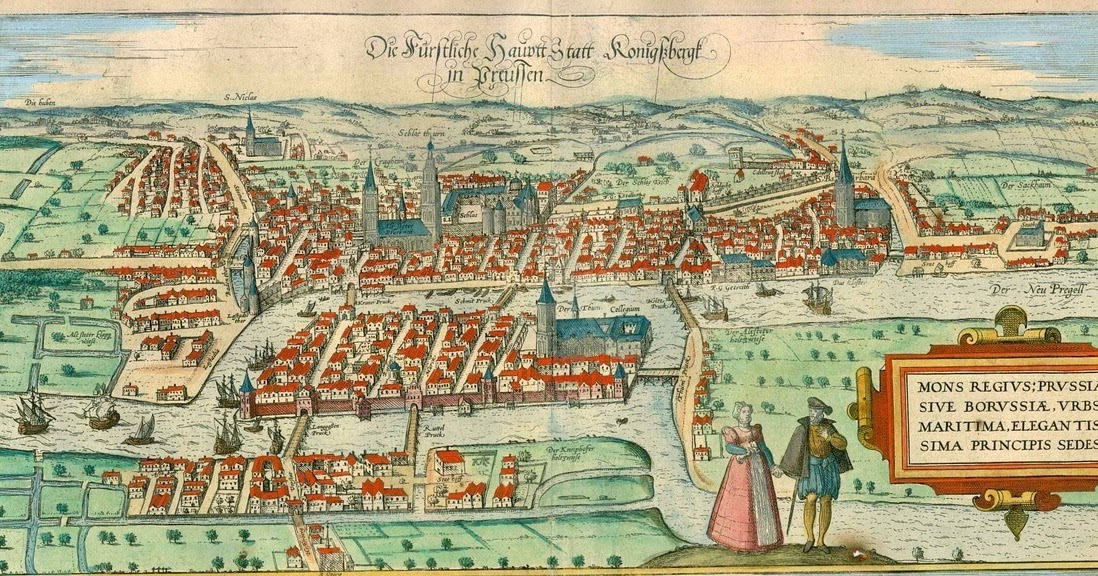
\includegraphics[width=0.4\textwidth]{Figures/Konigsberg.jpg}
\caption{ The map of K\"onigsberg } 
\label{fig:konigsberg}
\end{figure}

Let's highlight the number of bridges in the above map.
Let me give you another picture (copied from the internet) of
the bridges so that you don't have to suffer through the pixelated image.


\begin{figure}[ht]
\centering
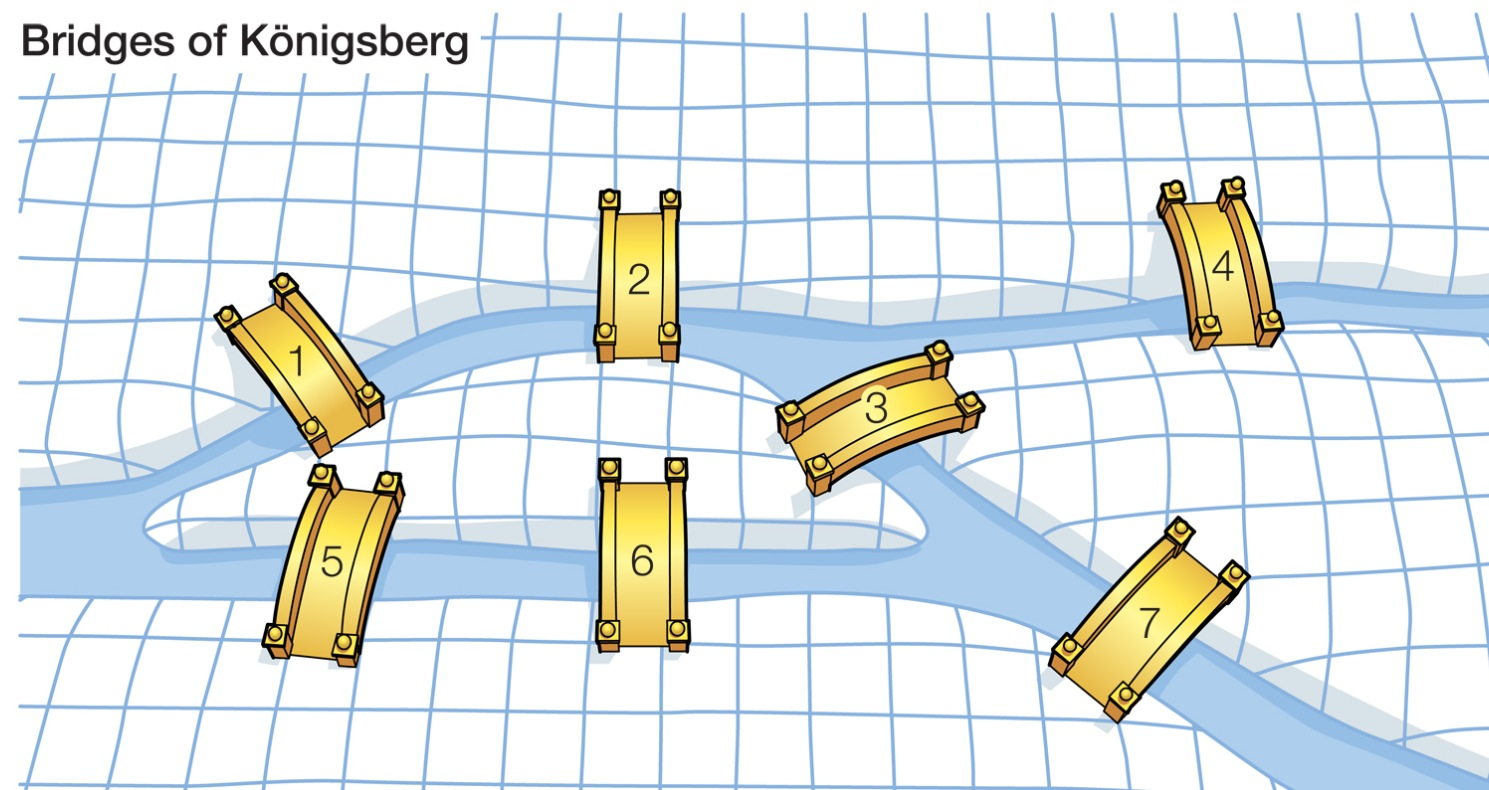
\includegraphics[width=0.4\textwidth]{Figures/Konigsberg-2}
\caption{ Bridges of K\"onigsberg } 
\label{fig:konigsberg-2}
\end{figure}

So you see there are 7 bridges.
According to lore, people in this city would spend Sunday afternoons to walk around
the city and to keep their thoughts occupied, they invented a game: find a path
to walk around the city, crossing each of the bridges only once.
It was an insanely difficult problem as perhaps none of the citizens was able to find a way to do it.

\begin{question}
    Try for 10 minutes to an hour to find a path around the city that crosses each
    bridge only once.
\end{question}

Leonhard Euler, perhaps the most prolific mathematician of all time, was asked this problem and 
thought it had nothing to do with math. But the more he thought about it, the more he was intrigued.
As a result, he invented two fields of mathematics, which are very fundamental to modern world: graph theory and topology.


Before going to talk about the problem, let me give an excerpt from an 
article on the Mathematical Association of America.
\footnote{
\url{https://www.maa.org/press/periodicals/convergence/leonard-eulers-solution-to-the-konigsberg-bridge-problem}
}

\begin{displayquote}
   Why would Euler concern himself with a problem so unrelated to the field of mathematics?  Why would such a great mathematician spend a great deal of time with a trivial problem like the Königsberg Bridge Problem?  Euler was obviously a busy man, publishing more than 500 books and papers during his lifetime.  In 1775 alone, he wrote an average of one mathematical paper per week, and during his lifetime he wrote on a variety of topics besides mathematics including mechanics, optics, astronomy, navigation, and hydrodynamics.  It is not surprising that Euler felt this problem was trivial, stating in a 1736 letter to Carl Leonhard Gottlieb Ehler, mayor of Danzig, who asked him for a solution to the problem:

    ``. . .  Thus you see, most noble Sir, how this type of solution bears little relationship to mathematics, and I do not understand why you expect a mathematician to produce it, rather than anyone else, for the solution is based on reason alone, and its discovery does not depend on any mathematical principle.  Because of this, I do not know why even questions which bear so little relationship to mathematics are solved more quickly by mathematicians than by others.''

Even though Euler found the problem trivial, he was still intrigued by it.  In a letter written the same year to Giovanni Marinoni, an Italian mathematician and engineer, Euler said,

    ``This question is so banal, but seemed to me worthy of attention in that [neither] geometry, nor algebra, nor even the art of counting was sufficient to solve it.''

Euler believed this problem was related to a topic that Gottfried Wilhelm Leibniz had once discussed and longed to work with, something Leibniz referred to as geometria situs, or geometry of position.  This so-called geometry of position is what is now called graph theory, which Euler introduces and utilizes while solving this famous problem. 
\end{displayquote}

I hope you tried the problem out for a good ten minutes. 
It's worth trying to think about the problem as you will have a feel of what's going on
and experience the historic walk in a  city with changed name.
It is not a conincidence that the citizens of K\"onigsberg tried for a long time
and did not succeed. It is impossible to find such a path!

Euler, as clever as he was, realized that usual ways of mathematical thinking
will not solve this problem.
He then, out of thin air, invented an entirely new way to think about it and proved that it is impossible to solve this problem, settling the game for the citizens (which means they will have to invent a new game to play...).
Let's see how he did it!

The following solution is copied from the book~\cite{Burger2013} as the argument 
there  is a direct application 
to Euler's abstract thinking without any abstract theorem.

\begin{proof}[Solution to the K\"onigsberg problem~\cite{Burger2013}]
   The shapes of the landmasses don't matter either, so we can simply replace each landmass by a dot. In fact, the only relevant features are the connections between the landmasses. That is, we focus on which landmass is connected to which other one by a bridge. Each bridge creates a connection between two landmasses.




\begin{figure}[h]
\centering
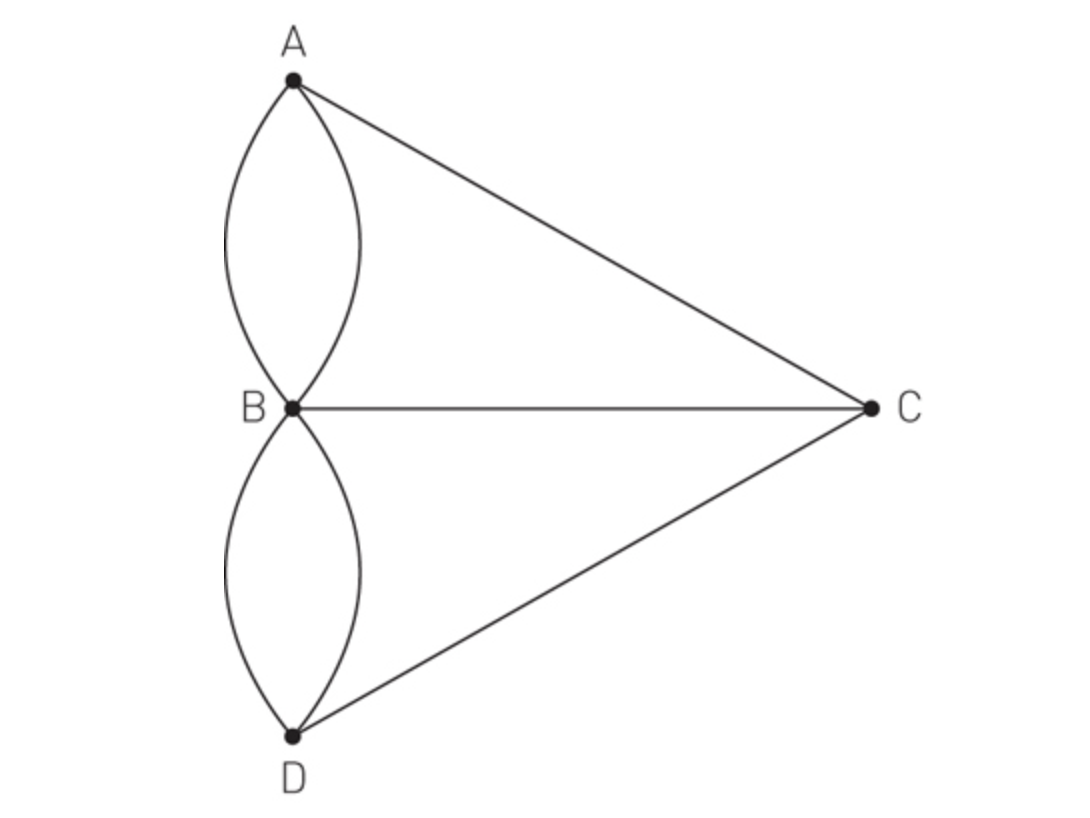
\includegraphics[width=0.4\textwidth]{Figures/Konigsberg-graph}
\caption{ The map of K\"onigsberg in graph form } 
\label{fig:konigsberg-graph}
\end{figure}

Now we are well on our way to isolating the essential features of the Königsberg Bridge Puzzle. We have a collection of places (landmasses now denoted as dots) and some pairs of them are connected (bridges now denoted as arcs between pairs of dots)—and these places and connections are all that matter for the challenge at hand. We could name the places A, B, C, and D. And we could describe the connecting bridges by writing which pair of places each bridge connects. So the seven bridges of Königsberg can now be denoted as AB, AB, AC, BC, BD, BD, and CD.





After we've stripped away all the unnecessary diversions, we could restate the Königsberg Bridge Puzzle as follows: Suppose we have four dots named A, B, C, and D, and we have seven connections among them, namely, AB, AB, AC, BC, BD, BD, and CD. Can we start at some dot and choose connections to take us from dot to dot in such a way that we use every connection exactly once and we return to the dot at which we started? Notice that the starting place does not matter; that is, if we could solve the puzzle starting at some dot we could also solve it starting from any other dot. Why is this true?

It might, at first, appear that we have not really made any progress toward solving the puzzle, but we have isolated the essential ingredients, and that is an enormous step forward. In fact, those essential ingredients—dots and connections—are the essential ingredients that comprise a modern mathematical area called graph theory. A graph is simply a set of vertices (that is, the dots) together with a collection of connections of pairs of the vertices (that is, the lines or arcs connecting pairs of dots). The connections are called edges. So the graph associated with the Königsberg Bridge Puzzle has vertices A, B, C, and D and edges AB, AB, AC, BC, BD, BD, and CD. Our simple picture that just shows the vertices and edges has all the information we require to tackle the Königsberg Bridge Puzzle. Now we can restate the Königsberg Bridge Puzzle as follows: Can we start at some vertex in the Königsberg graph, then choose edges to take us from vertex to vertex in such a way that we use every edge exactly once and we return to the vertex at which we started?

The Königsberg graph shows us that there are four landmasses (represented by the vertices) and it shows which landmasses are connected by bridges (represented by the edges). By the way, the order of the vertices that describe an edge does not matter; in other words, CD and DC both mean the same thing, namely, a “bridge” (or edge) connecting landmasses C and D. Since two bridges connect A to B and two bridges connect B to D, we simply list AB twice and BD twice, but we don't make any attempt to distinguish the two AB bridges from one another. For example, we don't care which AB is the bridge nearer D. We make no distinction between the two AB edges, because an edge is just a connection between its vertices. No other feature of an edge matters, such as how or where we draw it.

If we take a walk over the edges of the Königsberg graph, we can represent that walk by the ordered sequence (list) of edges that we traversed. For example, if we just go from A to B to D to C to B and back to A, we could represent that walk by listing the edges (AB)(BD)(DC)(CB)(BA) in the given order. Notice that it doesn't matter which of the two BD edges we choose, as each one accomplishes the same task of getting us from B to D.


Suppose we take a walk around the Königsberg graph and return back to where we started. If we write down the ordered sequence of edges involved, notice that each edge that we traverse must start at the point at which the previous edge ended. So in our example (AB)(BD)(DC)(CB)(BA), after we traveled along one of the edges from A to B, the next edge of course started at B and ended at some other point, in this case D. Then we took an edge from D to C, then journeyed on the edge from C to B, and then went from B to A using the edge we didn't use the first time. Since we returned to the place where we started, the first letter and the last letter will coincide.


Let's forget the parentheses and just look at the letters that are written down in our list of the edge-sequence, namely, ABBDDCCBBA. Notice that every letter appears an even number of times, because every internal letter is the end of one edge and therefore, in turn, the beginning of the next edge, so every internal letter appears in pairs, while the first and last letters are the same (because we return to where we started), so that letter appears in pairs as well. 
The list of edges of such a circuit is the Noah's Ark of graph theory: Every letter appearing comes in pairs, in this example: BB, DD, CC, BB, and of course our starting and ending location AA.

This observation about letters appearing an even number of times lets us solve the Königsberg Graph Puzzle. Why? Well, let's look at the list of all seven edges of Königsberg. They are AB, AB, AC, BC, BD, BD, CD. If we walked over all the Königsberg edges each exactly once in any order at all, those seven pairs of letters would be the ones describing our walk. It might start (AB)(BC)(CD)… and so on. But if each edge in the Königsberg graph (that is, each given pair of letters such as AC) appeared exactly once in our walk, then the total number of A's would be 3 (an odd number), because we can see that there are exactly three A's in our seven edges—namely one A each in the edges AB, AB, and AC, and no other A's in any of the other edges. Similarly, the total number of B's would be 5, the number of C's would be 3, and the number of D's would be 3.

But we saw that if we were able to take a walk over the edges—traversing each edge exactly once—and return to where we started, then when we recorded the edges in the order that we walked over them, each letter would appear an even number of times. But this even number of appearances of each letter is impossible for the Königsberg graph because we just noticed that each letter appears an odd number of times on our list of bridges. Thus we conclude that it is impossible to start at one location, traverse each and every edge exactly once, and return to our starting point.

This observation settles the Königsberg Graph Puzzle and thus settles the Königsberg Bridge Puzzle, definitely proving that it is impossible to walk over each bridge just one time. Please think through the reasoning and “bridge” the ideas of the argument together for yourself until every step makes sense.
\end{proof}

\section{Graph theory}

Let us recap some essential ideas in the above argument 
and turn them into mathematical symbols.
\begin{definition}[Graph]
    A \emph{graph} $G = (V,E)$ consists of a set $V$ of \emph{vertices} (or \emph{nodes})    
    and a set $E$ of \emph{edges}.
    
    An \emph{edge} in a graph is a curve that has endpoints connecting a vertex to another 
    vertex or a vertex to itself.
    
    A \emph{loop} in a graph is a curve that connects a vertex to itself.
\end{definition}

There are various ways to represent vertices and edges. One way is just to draw out
the graph as in Figure~\ref{fig:konigsberg-graph}.
Another way is to just write down the list of vertices in a set such as
\begin{equation*}
    \set{A,B,C,\dots} \,,
\end{equation*}
and a list of edges and loops connecting the vertices by writing the vertices next to each other such as
\begin{equation*}
    \set{AB, AA, BC, BA, \dots} \,.
\end{equation*}

\begin{definition}[Path]
    A \emph{path} is a succession of edges of the form $v_1v_2,v_2v_3,\dots, v_n v_{n+1}$ so that
    all the edges and vertices only appear once when drawn out.
\end{definition}
\begin{definition}[Connected graph]
    A graph $G = (V,E)$ is called \emph{connected} if, for any pair of vertices $A, B \in V$, there is a path from $A$ to $B$.
\end{definition}


\begin{definition}[Eulerian path]
    An \emph{Eulerian path} is a path through a graph which traverses each 
    edge exactly once.
\end{definition}

\begin{definition}[Eulerian cycle]
    An \emph{Eulerian cycle} is an Eulerian path that ends in the same vertex where it started.
\end{definition}


\begin{definition}[Degree]
    In a graph $G = (V,E)$, the \emph{degree} of a vertex $A$, denoted by $\deg(A)$
    is the number
    of edges that connect to $A$, and loops (i.e. edges $AA$) are counted twice. 
\end{definition}




\begin{theorem}
    Let $G$ be a finite connected graph. Then an Eulerian path exists if and only if there are at most two vertices with odd degree, and if there are, vertices of odd degrees must be the start or the end of the path. An Eulerian cycle exists if and only if all vertices have even degrees.
\end{theorem}






%%%
\section{Coloring maps and what graphs have to do with it}
%%%

%%%
\subsection{Motivation}

\paragraph{Acknowledgement:} This lecture is based on material shared by Renee Bell and Patrick Shields.

\begin{question}
    If you take a world atlas and pick a region, what is the minimal number of colors you would need to color every country in a way that each pair of countries that share a borderline has different colors?
\end{question}

You can try, unsuccessfully, to color Central America with two colors. Try it and notice how you run into trouble around the point where three countries come together, for example Mexico, Belize and Guatemala:

\begin{center}
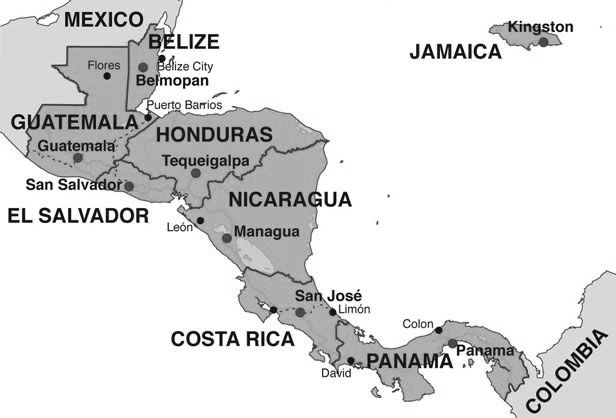
\includegraphics[width=7cm]{pics/central-america-uncolored.jpg}
\end{center}


However, it \textit{is} possible to color this map using three colors:

\begin{center}
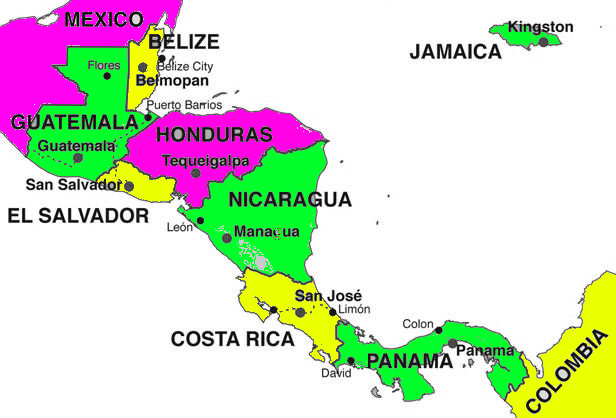
\includegraphics[width=7cm]{pics/central-america-colored.png}
\end{center}


Alright, maybe we can do this for all maps using 3 crayons. Let's consider the following map of the planet of Chromatica, which is in another galaxy, and has countries A,B,C, and D.

\begin{center}
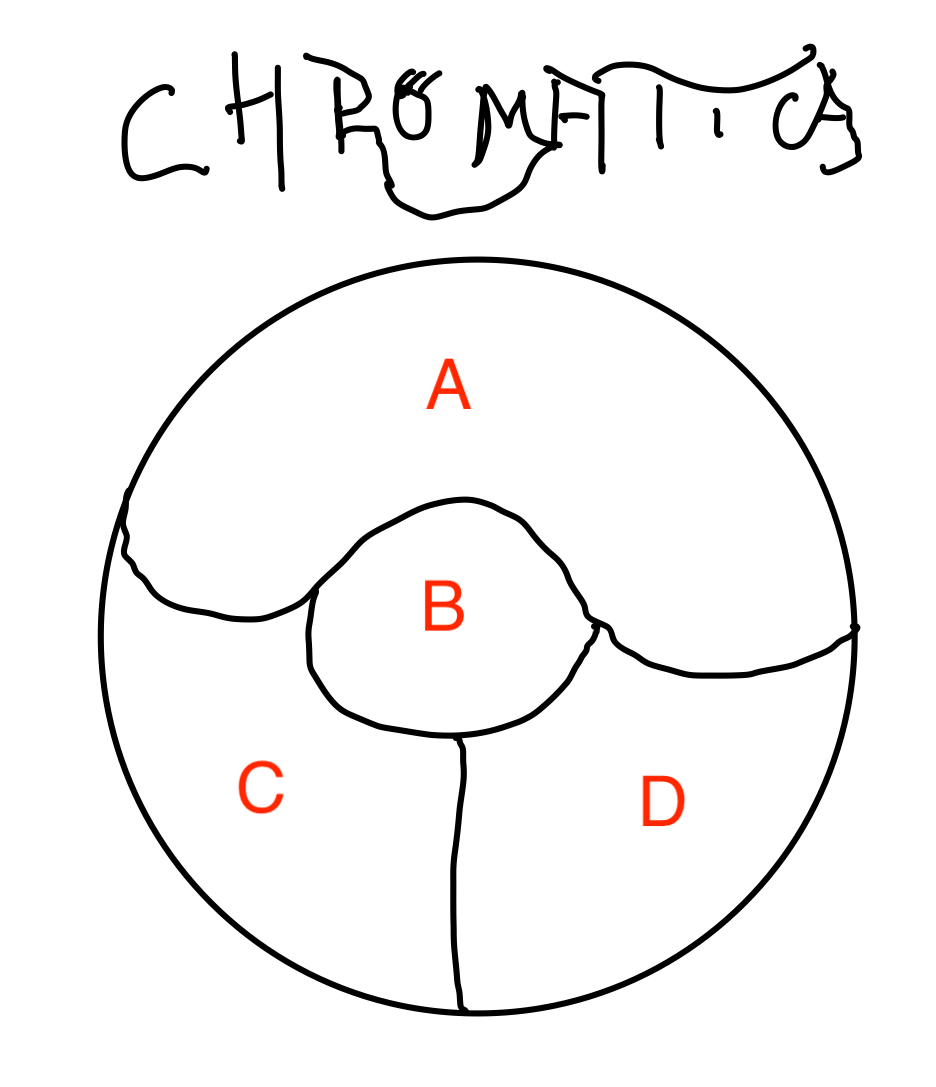
\includegraphics[width=7cm]{pics/chromatica-uncolored.png}
\end{center}

\begin{question}
Can you find a coloring of Chromatica which uses only three colors?
\end{question}

In this case, even three is not enough! If we color A pink, then neither C nor D can be pink, since they're touching A. But C and D cannot be the same color, since C is touching D. So, let's say C is green and D is yellow. Then B is left touching a pink state, a green state, and a yellow state. So it can't be any of those colors. We will need a fourth color, let's say blue.

\begin{center}
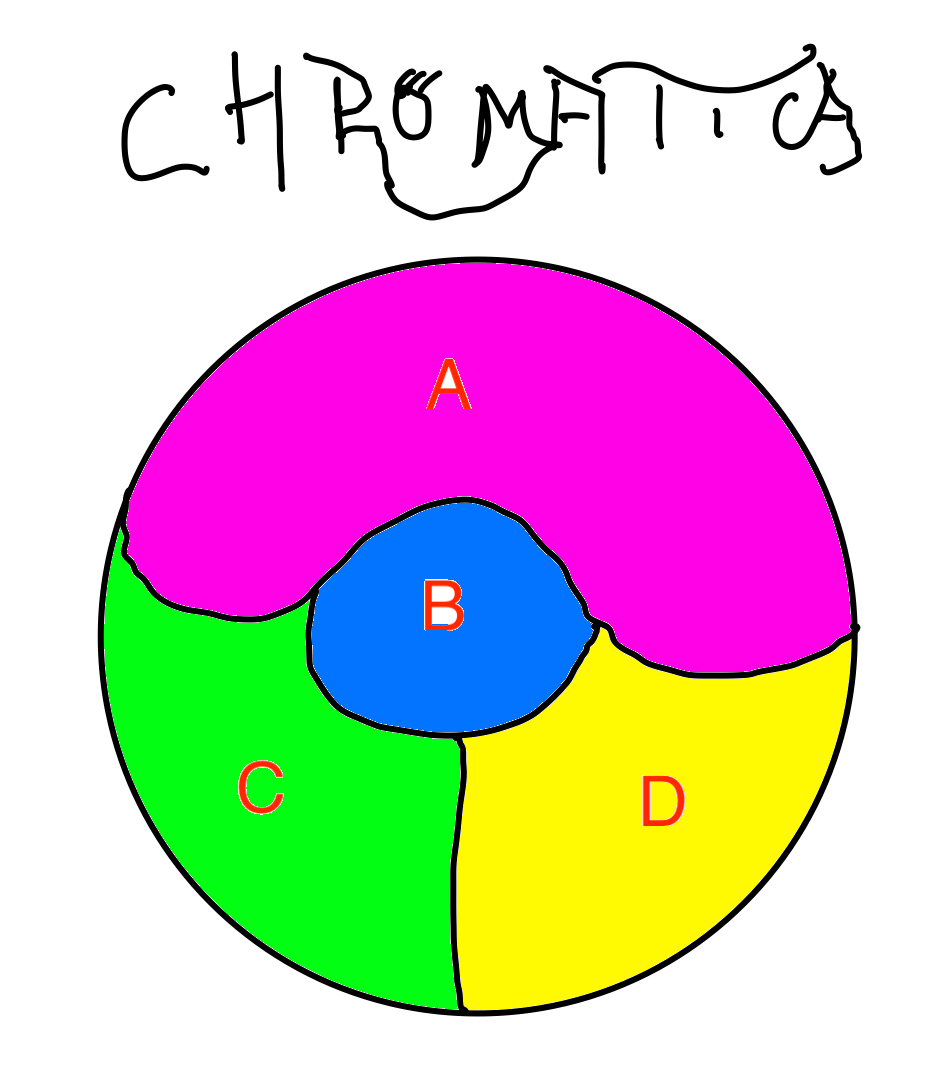
\includegraphics[width=7cm]{pics/chromatica-colored.png}
\end{center}

Could there be a map where even four colors isn't enough?
It turns out the answer is no, but it took a long time to prove that decisively. The conclusive answer to this question was given by Kenneth Appel and Wolfgang Haken in 1976, in the form of the following theorem, called the Four Color Theorem.

\begin{theorem}[Four Color Theorem for Maps]
Every map can be colored such that no two regions which share a boundary are the same color, using four colors.
\end{theorem}


%%%
\subsection{Graphic content}

Now let's try to abstract and simplify this problem, especially for people who are not great at drawing countries.
The only information we needed was which countries share a boundary! So let's record that information using a graph.\\

We create a graph associated to this map, with a vertex for each country and an edge between two vertices if the associated countries share a boundary. Here are the graphs for Central America and Chromatica:

\begin{center}
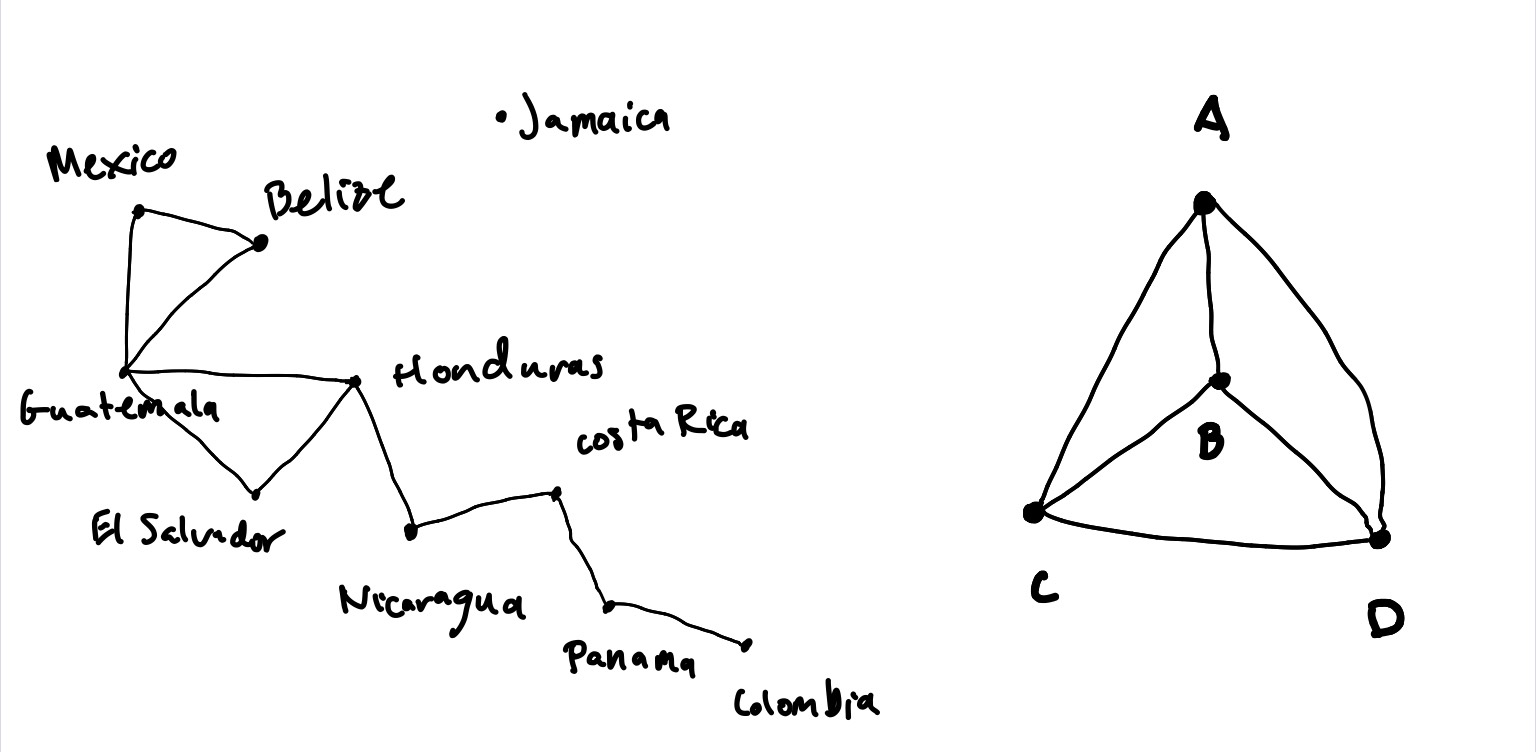
\includegraphics[width=11cm]{pics/map-graphs.jpeg}
\end{center}

Now the question reduces to coloring the \textit{vertices} of these graphs so that no two vertices which share an edge are the same color. Let's formalize this in a definition:

\begin{definition}
A \textbf{coloring} of a graph is a labeling of the graph’s vertices with colors such that no two vertices sharing the same edge have the same color.
\end{definition}

If you don't have a lot of colors at your immediate disposal, you can label colors by numbers, symbols, letters of Japanese alphabets, whatever suits your tastes better.

Here are the colorings of the graphs associated to Central America and Chromatica corresponding to the map colorings we just did:

\begin{center}
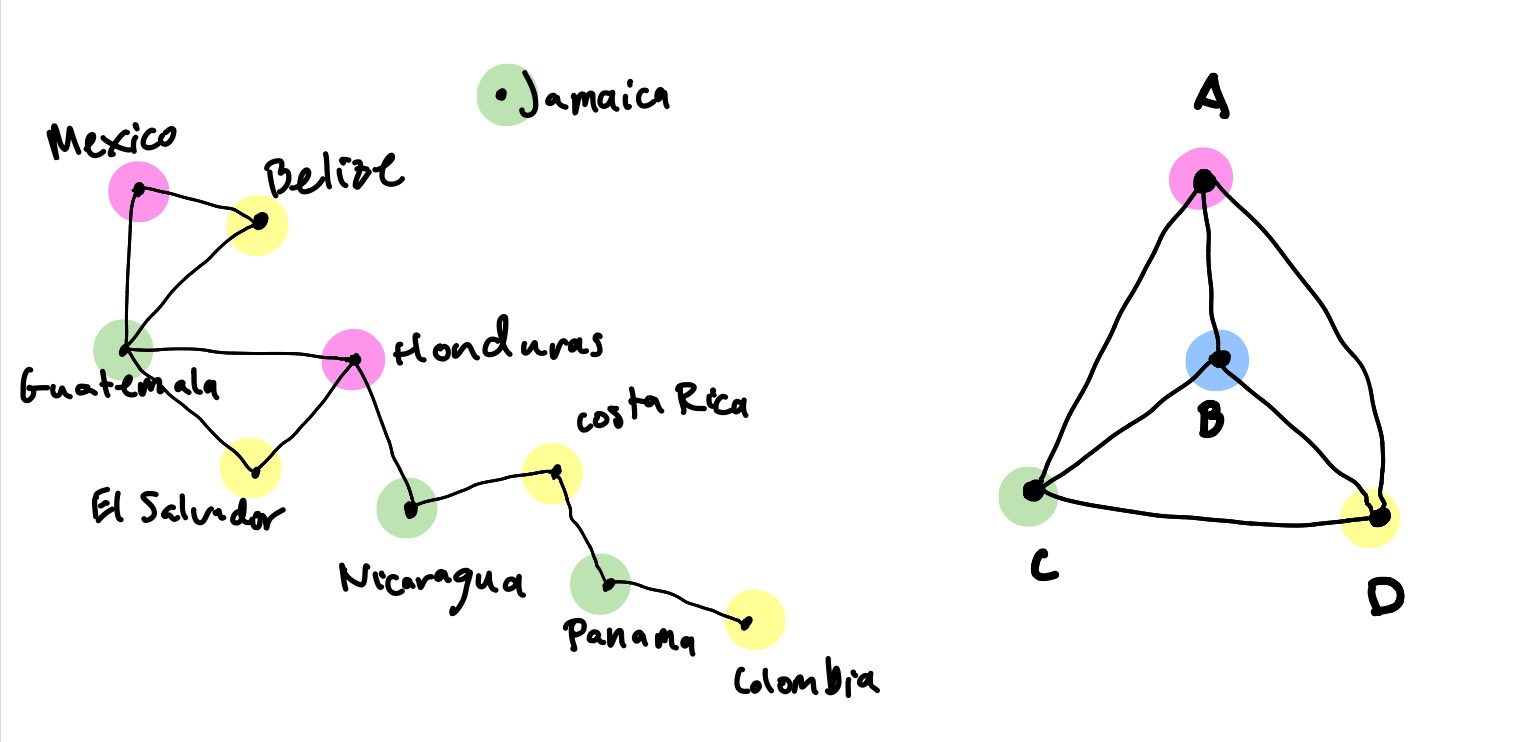
\includegraphics[width=11cm]{pics/map-graphs-colored.jpeg}
\end{center}

We're also trying to figure out the number of colors we need to do this. This motivates the following definition:

\begin{definition}
A coloring using $k$ colors is called a  $k$-\textbf{coloring}. The smallest number of colors needed to color a graph $G$ is called its \textbf{chromatic number}, and is denoted $\chi(G)$.
\end{definition}

In the examples we just saw, $\chi$(Chromatica)$=4$, since we can color it using four colors but NOT using fewer. We also calculated that $\chi$(Central America)$=3$.\\ 

The definitions we just gave could be for any kind of graph. For example, the pentagram, which we will call $P$:

\begin{center}
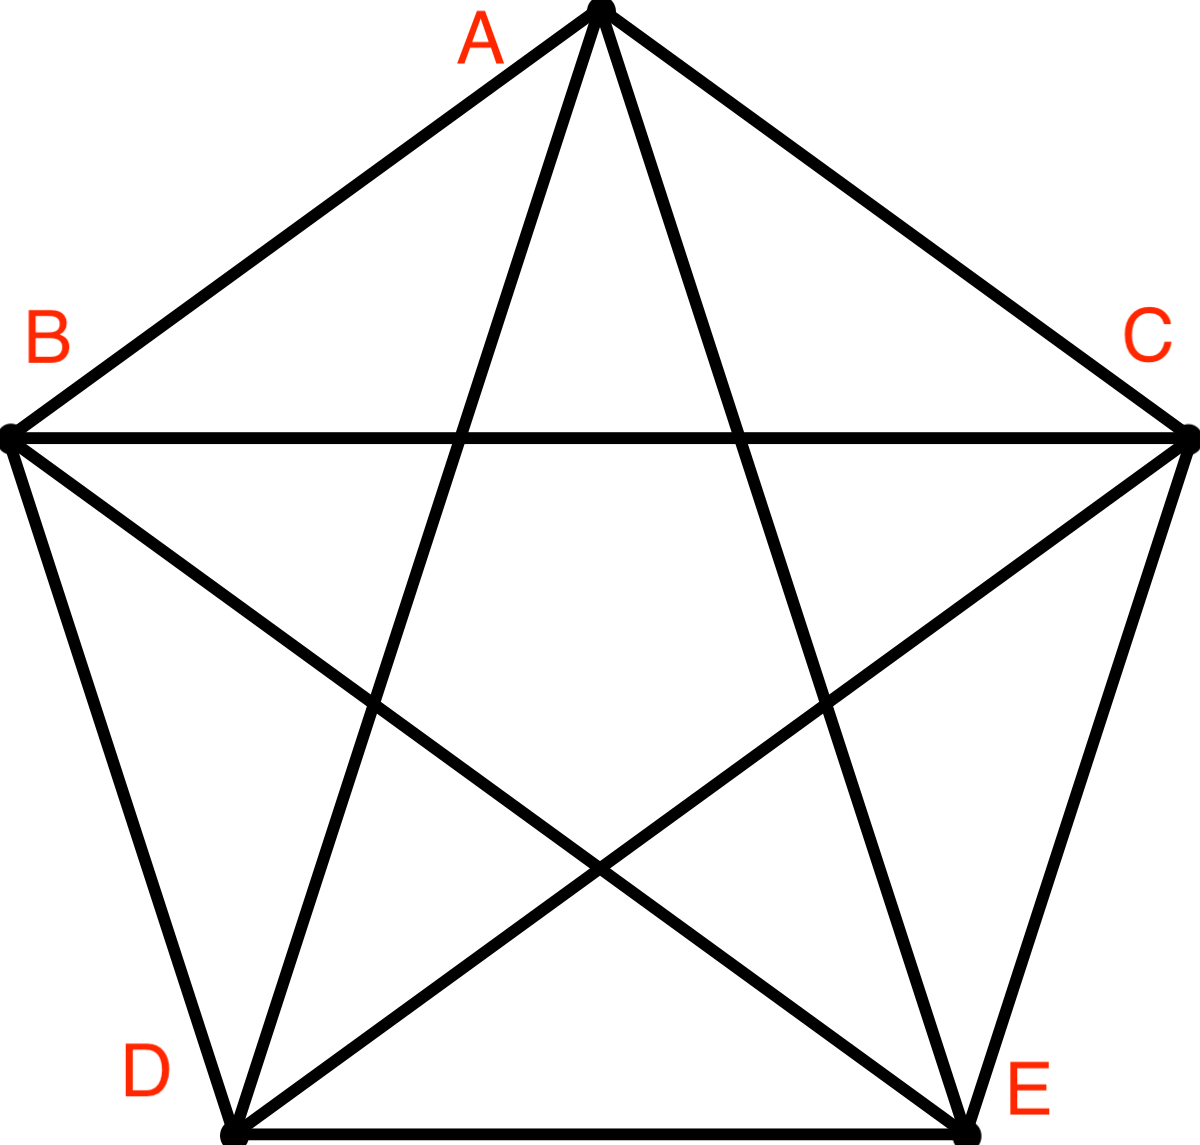
\includegraphics[width=6cm]{pics/Pentagram.png}
\end{center}

Let's calculate its chromatic number. Of course, we could 5-color it by just making every single vertex a different color, so we know $\chi(P) \leq 5$. 
So, can we color it using four colors? Well, let's say we color A ``color 1''. Since B shares an edge with A, it must be a new color, ``color 2''. Since C shares an edge with both A and B, it must be a new color, ``color 3''. D must be a fourth color, ``color 4''. And finally, E touches every other vertex, so it must be a fifth color. $P$ cannot be colored using 4 colors, so $\chi(P) = 5$.\\



But wait, didn't we just say that four colors is enough? Well, that was only for \textit{maps} which are ``2-dimensional'' in some sense, not \textit{all} graphs. The type of graph that we made is called \textbf{planar}.\\

\begin{definition}{}
A graph is \textbf{planar} if it can be drawn on the plane (that is, in two dimensions) in such a way that its edges intersect only at their endpoints.
\end{definition}

We can now give a different version of the Four Color Theorem:

\begin{theorem}[Four Color Theorem for Graphs]
Every planar graph can be 4-colored.
\end{theorem}

Now we see that the problem with the pentagram is that it's not planar; it can't be ``untangled'' into a nice 2D graph that lies flat in the plane.
\\

%%%
\subsection{Conflict Resolution}

I realize that not all of you are planning to become cartographers, but most of us have to deal with conflict sometimes, so let's look at a more likely application.
Suppose you are planning a small dinner, now that the worst of the lockdown is over, and want to determine a seating chart, seating people at different tables.
You are inviting your friends Jane, Matt, Imani, Hyunjeong, Bessam, Padma, and Alejandro. You love them dearly, but they are very... passionate people, and you know that if you seat two of them who disagree at the same table, the dinner is going to go very badly. Here are their conflicts:
\\

Matt and Imani are Patriots fans. Jane and Padma are Eagles fans. 
Do not sit them next to each other! Also, Hyunjeong likes Cardi B but Alejandro and Bessam are hardcore Nicki Minaj stans (barbz), so she won't sit with either of them. Alejandro dated both Matt and Jane so he doesn't want to sit with them, because that would be awkward. Other than that, everyone is cool. Let's list the conflicts:
\begin{enumerate}
    \item Matt can't sit with Jane
    \item Matt can't sit with Padma
    \item Imani can't sit with Jane
    \item Imani can't sit with Padma
    \item Hyunjeong can't sit with Bessam
    \item Hyunjeong can't sit with Alejandro
    \item Alejandro can't sit with Jane
    \item Alejandro can't sit with Matt
\end{enumerate}

We can record this information in the following chart:
\begin{center}
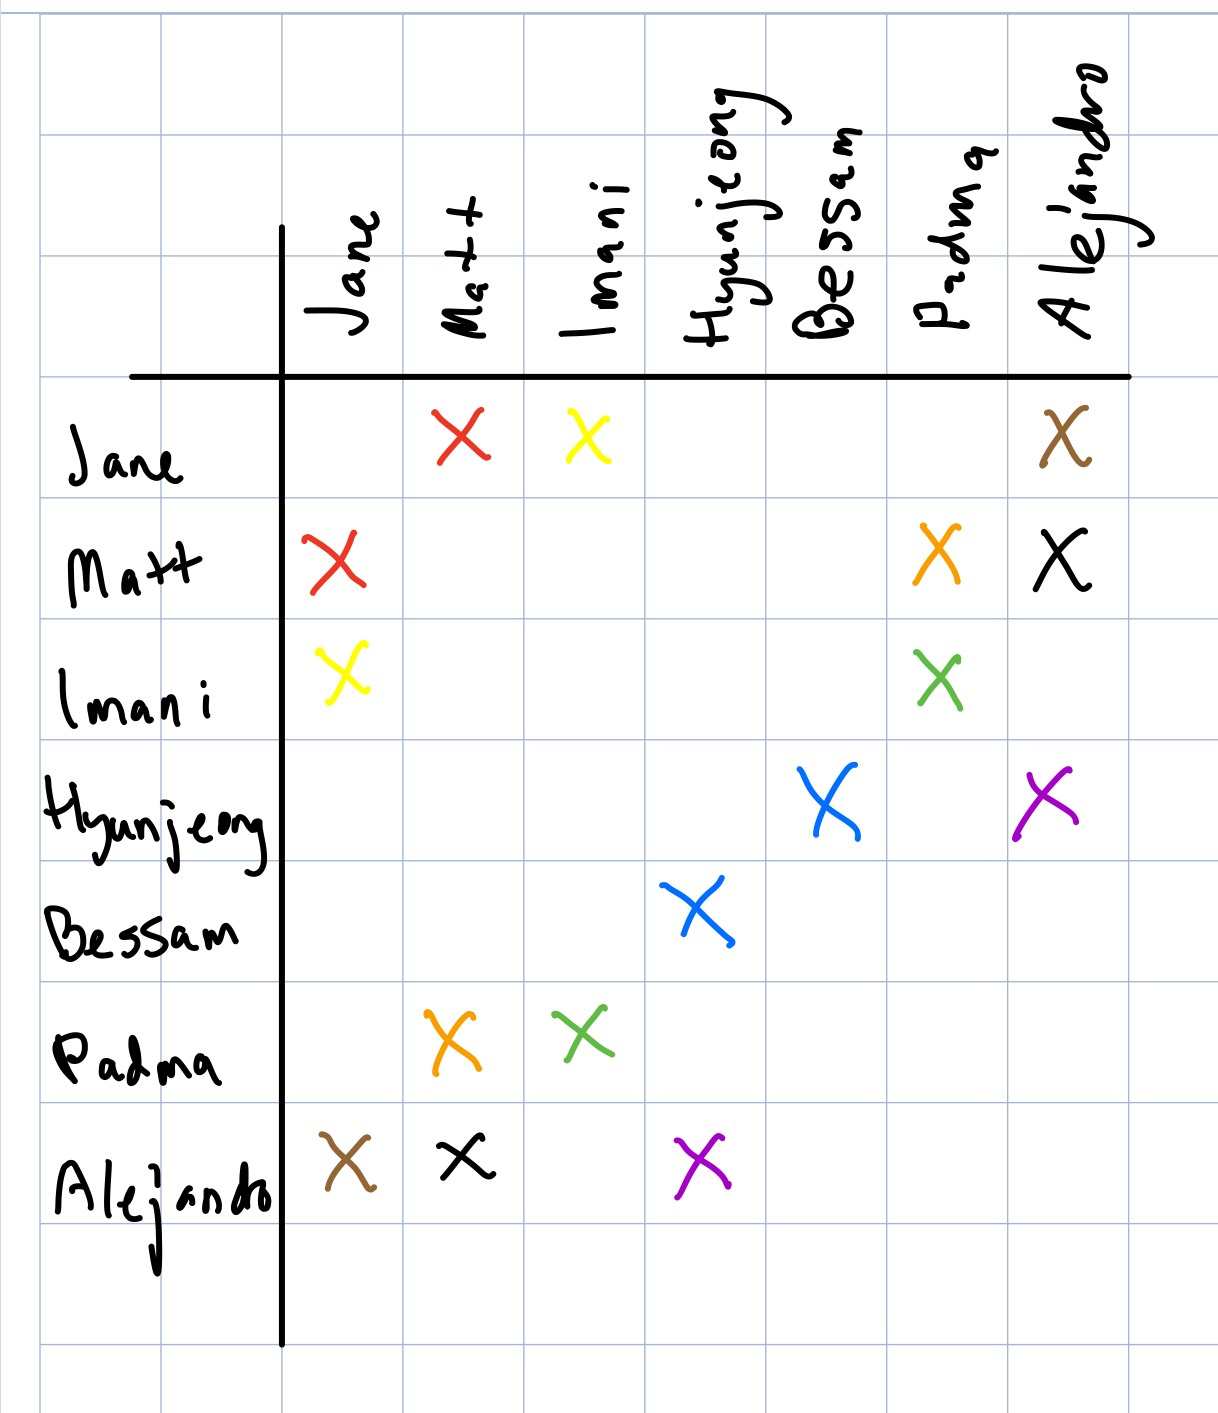
\includegraphics[width=7cm]{pics/dislike-chart.jpeg}
\end{center}

This is a very neat, excel-spreadsheet style way to record the information. But we can also record it in a graph. The only thing that matters for us is whether or not any two people have conflict. So we can create a graph where the vertices represent people, and there is an edge between two people if there is conflict between them.
We show this with the colors corresponding to the conflicts on the left, and in black and white on the right. We will not really need to color the edges, but we will have to color the vertices.

\begin{center}
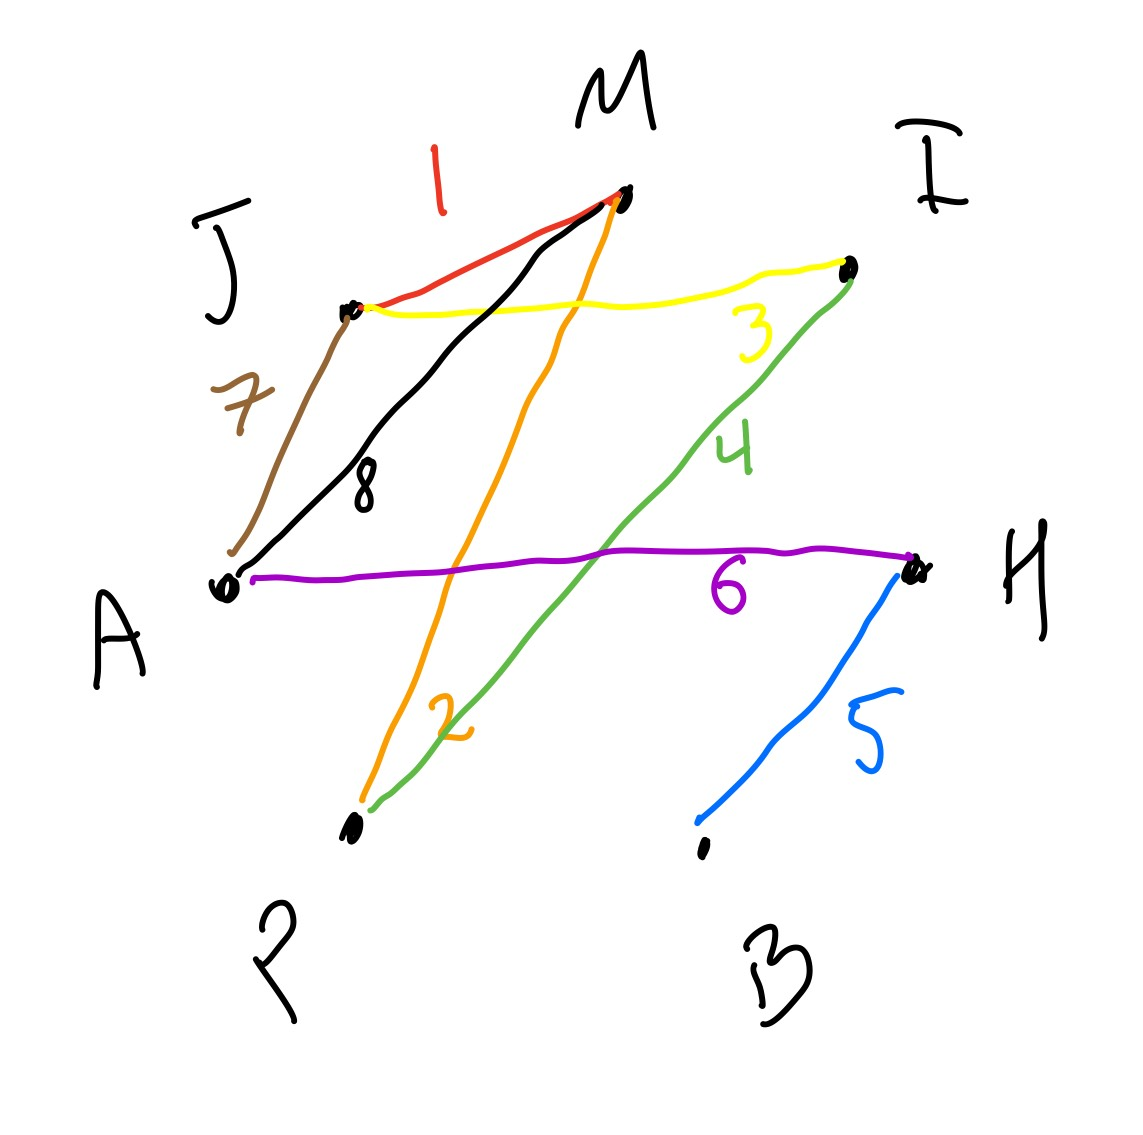
\includegraphics[width=6cm]{pics/conflict-graph.jpeg}
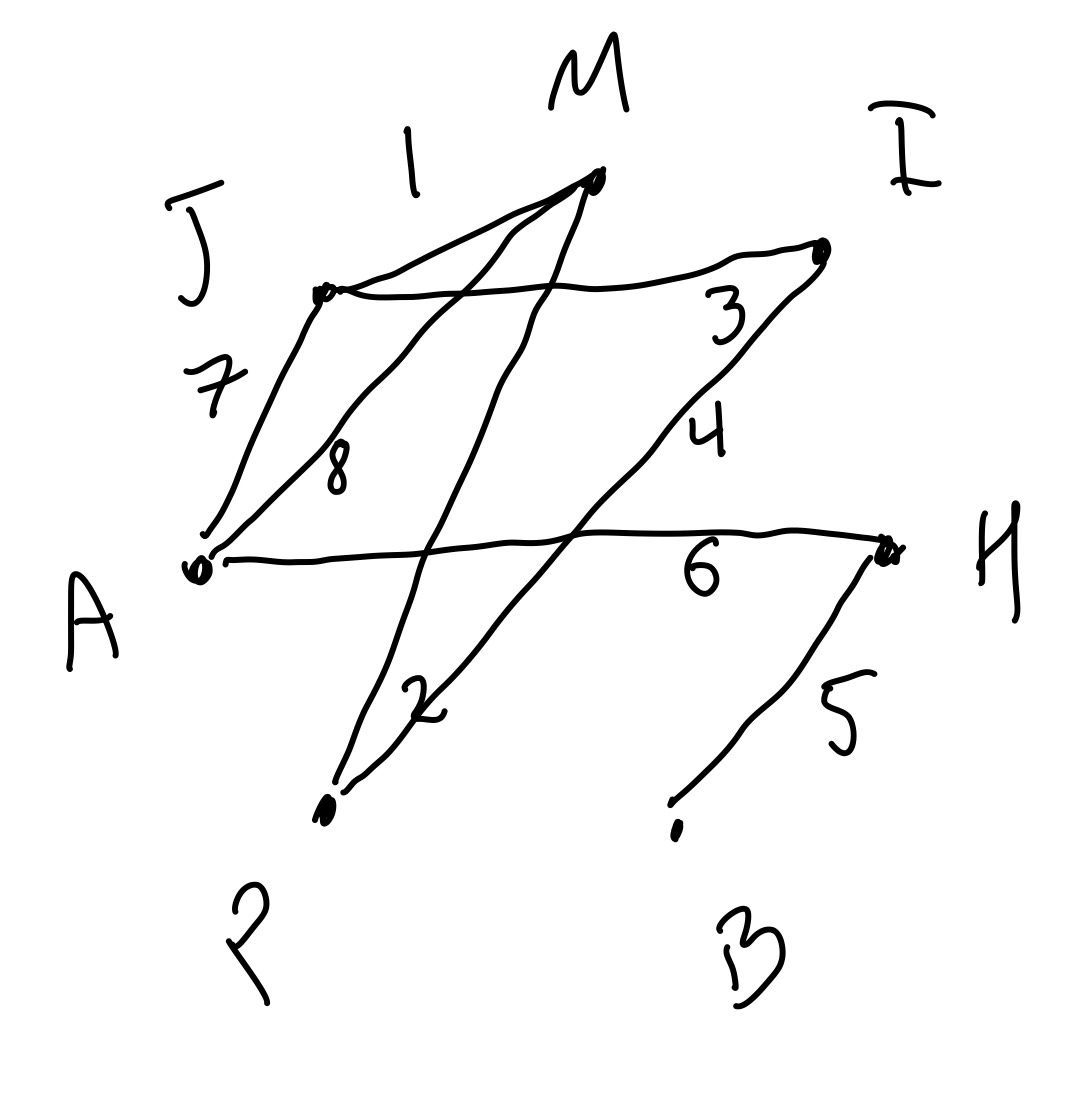
\includegraphics[width=6cm]{pics/conflict-graph-bw.jpeg}
\end{center}

\begin{question}{}
How can you figure out how many tables you will need for your dinner using this graph?
\end{question}

We just learned a new thing we can do with graphs, which is color them. You can think of a coloring using $k$-colors as a way of putting the vertices into $k$ groups, where no group has any two vertices which share an edge. 

Conversely, if we put the vertices into $k$ groups, where no group has any two vertices which share an edge, we can use that to make a $k$-coloring for the graph! We just pick a color for each group, and then color the vertices in each group accordingly.


Back to the dinner; we can find a 3-coloring of the graph using red, yellow, and blue as follows:

\begin{center}
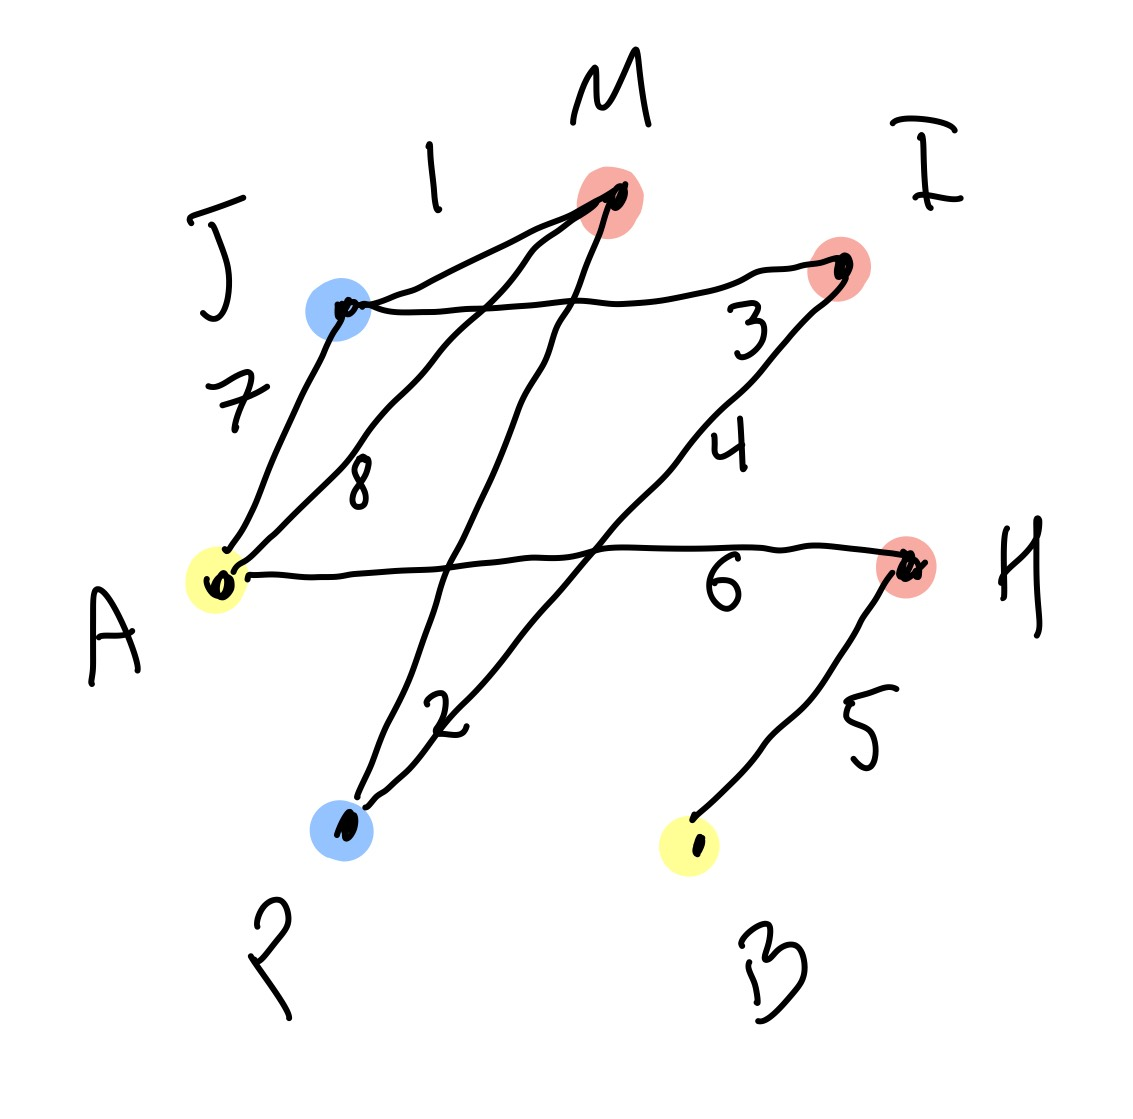
\includegraphics[width=8cm]{pics/conflict-3-colored.jpeg}
\end{center}

This allows us to seat everyone using 3 tables! You can refer to tables as the red table, the yellow table, and the blue table. The graph above corresponds to the following seating:

\begin{center}
\begin{tabular}{c|c}
 \multicolumn{2}{c}{Tables}\\
\hline
 Color & Vertices of that color \\
 \hline
 \hline
 Red & Matt, Imani, Hyunjeong\\
 \hline
  Yellow & Alejandro, Bessam \\
 \hline
  Blue & Jane, Padma \\
 \end{tabular}
 \end{center}
 
 You can check that this graph can't be 2-colored. This means there's no way of seating everyone at 2 tables without there being some conflict. Better bring enough tables!\\
 
\subsection{Scheduling}
Let's look at one \textit{final} application: scheduling final exams. 
Suppose we're scheduling exams for Math, Computer science, French, Sociology, Biology, and Anthropology.
We'll make a graph where the vertices are subjects, and there is an edge between two vertices if the corresponding subjects have a conflict.\\

Suppose that Student 1 is in Math, French, and Sociology.
This means that Math and French are in conflict, French and Sociology are in conflict, and Math and Sociology are in conflict (since this student can't attend both exams at the same time).
So there is an edge between Math and French, an edge between French and Sociology, and an edge between Sociology and Math.


Suppose also that
Student 2 is in Anthropology, French, and Sociology, Student 3 is in Biology and Computer science, Student 4 is in Computer science and Mathematics, and Student 5 is in Math and Anthropology.

This gives rise to the following graph, where the conflict edges are colored according to which Student is the cause of them:

\begin{center}
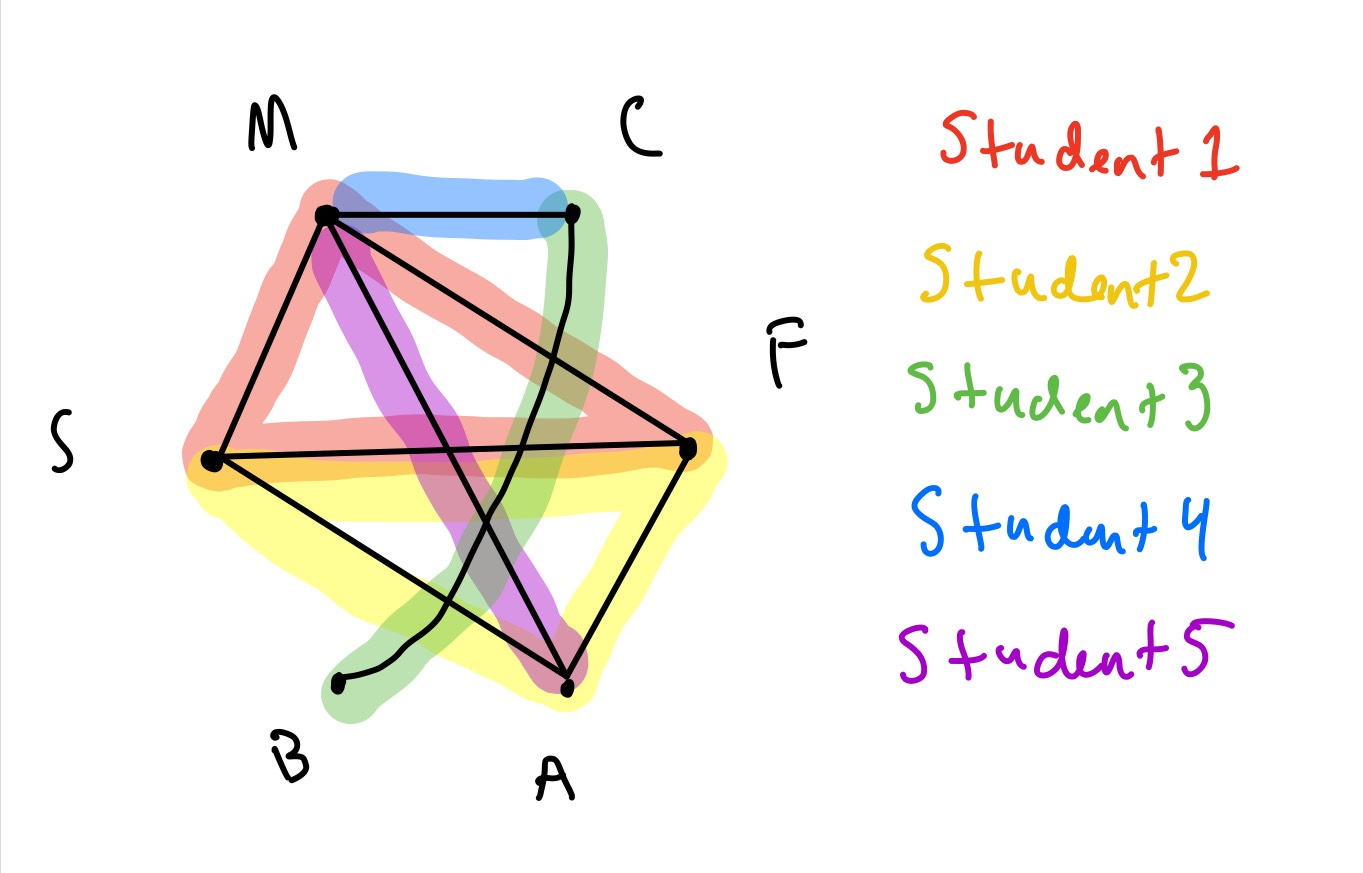
\includegraphics[width=11cm]{pics/final-conflicts.jpeg}
\end{center}

\begin{question}{}
How many timeslots do we need for these final exams? How can we pick which exams go in which timeslot?
\end{question}

Again, colorings of this graph correspond to conflict-free exam schedules. You can check that it's impossible to 3-color the graph (so we need more than 3 timeslots), but we can 4-color the graph as follows: 

\begin{center}
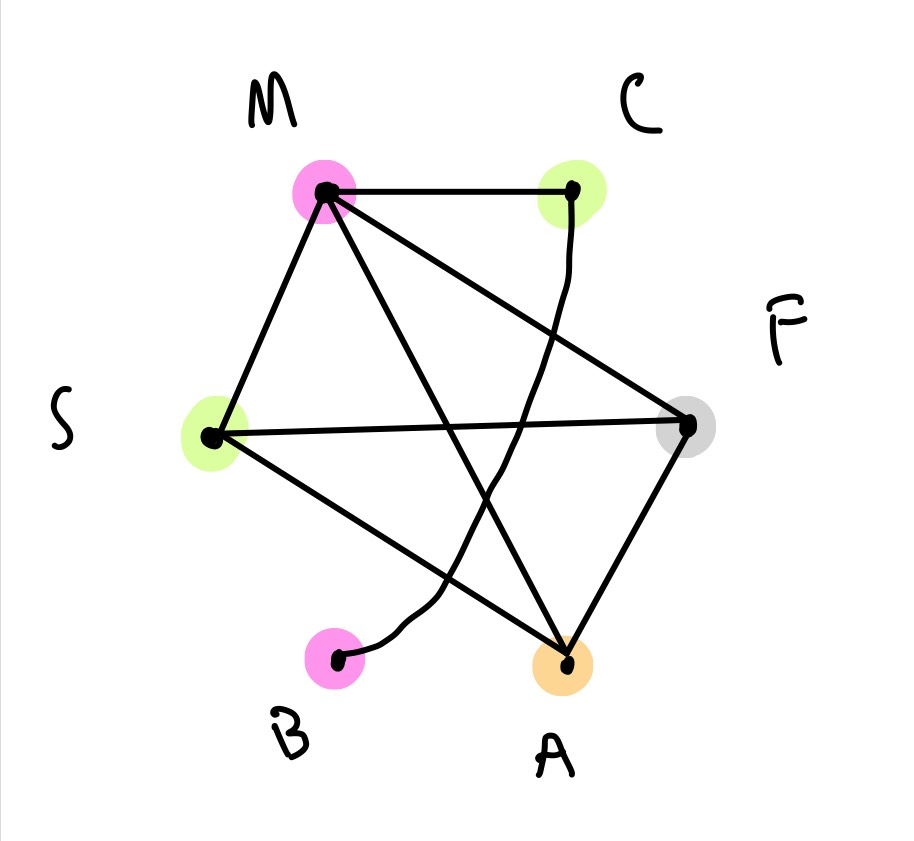
\includegraphics[width=5cm]{pics/final-coloring.jpeg}
\begin{tabular}{c|c}
 \multicolumn{2}{c}{Timeslots}\\
\hline
 Color & Vertices of that color \\
 \hline
 \hline
Hot pink & Math, Biology\\
 \hline
  Lime green & Computer science, Sociology \\
 \hline
 Grey & French \\
 \hline
 Orange & Anthropology
 \end{tabular}
 \end{center}
 
Hence we can have Math and Biology in the first timeslot, Computer science and Sociology in the second timeslot, French in the third timeslot, and Anthropology in the fourth timeslot.



%%%
\section{Chromatic polynomial of a graph}
%%%

The previous section was motivated by a more applied thinking about graphs. In this section, we would like to discuss what mathematicians care about.

In general, when mathematicians define a certain kind of object -- geometric shape, function, graph, set -- we then ask a question about how to classify these objects. For example, for sets, we can count the number of elements (which may be infinite), and if two sets have the same number of elements, then there is a bijection between them, in other words, we can identify their elements. After suitable identifications, we can start asking what are significant distinctions between the objects. For example, to each we can assign a number, like the chromatic number for a graph. These numbers are called \emph{invariants}.

For graphs, one invariant that is closely related to the chromatic number is the \emph{chromatic function}.

\begin{definition}
Let $G$ be a graph. Then we define the \emph{chromatic function} $P_G: \N \to \N$ by the following rule:
$P_G(n)=$ the number of colorings of the vertices of $G$ into $n$ colors.
\end{definition}

Let us compute some examples.

\begin{example}
Let first $G$ be the graph with one vertex and no edges, so $V = \{A\}$ and $E = \varnothing$. It looks like a dot. Given $n$ colors, we can color this dot in exactly $n$ ways, one for each choice of color, so $P_G(n) = n$.
\end{example}

\begin{example}
Let us go a few steps further and set $G$ to be the graph with 3 vertices and no edges, so $V = \{A,B,C\}$ and $E = \varnothing$. It looks like three dots. Given $n$ colors, we can color the vertex $A$ in $n$ ways. Then we are free to choose any color for $B$, since it is not connected to any other vertices, so for each of the first $n$ variants, we have $n$ variants in turn, which brings us to $n^2$ variants. Finally, the third vertex $C$ is not connected to any others, so we can color it  in $n$ ways independently of the previous choices. In total, it brings us to $P_G(n) = n^3$. 
\end{example}

\begin{exercise}
Generalize the previous two examples as follows: if $G$ is a graph with $v$ vertices and no edges, prove by induction that $P_G(n) = n^v$.
\end{exercise}

Let us now consider a more involved example -- graphs that have not just vertices, but also edges. You may have already guessed that graphs with loops (edges that begin and end in the same vertex) cannot be colored at all. Indeed, if you have a loop $AA$, definition of coloring tells us that the color of the vertex on the one side of $AA$ cannot be the same as color of the vertex on the other side... but oh no, it is the same vertex! So we can ignore graphs with loops because for them the problem of counting is trivial. Furthermore, if you have multiple edges that connect the two vertices, say $A$ and $B$, then each of the edges gives the same condition -- that $A$ and $B$ should be colored differently. So we can also ignore all but one edge between $A$ and $B$. To sum up, from now on we can only consider graphs that don't have loops, and each pair of vertices shares at most one edge.

\begin{definition}
    A \emph{simple graph} is one in which there is at most one edge joining a given 
    pair of vertices and there are no loops (i.e. edges joining a given vertex with itself).
\end{definition}


\begin{example}
Let us consider a graph with $v$ vertices that looks like a string, we will call this graph $A_v$.

Let us start with $v=5$ vertices and count the number of colorings of this graph into $n$ colors, that is we will calculate the value $P_{A_5}(n)$. We'll first color the leftmost vertex -- for this, we have $n$ choices of colors. But when we pick a color for the second vertex, we notice that one color -- the color of the first vertex -- is no longer available. So we now have $n-1$ choices. Similarly, the third vertex is connected to one vertex which is already colored, yielding $n-1$ choices again, and same for the fourth and fifth vertex. So altogether, we get the following result:
$$ P_{A_5}(n) = n(n-1)^4 \,.$$
\end{example}

\begin{exercise}
Guess a formula for $P_{A_v}(n)$ and prove it by induction.
\end{exercise}


\begin{example}
\label{ex:coloring_square}
Now let us consider the graph that can be drawn as a square, let's call it $G$:

\begin{center}
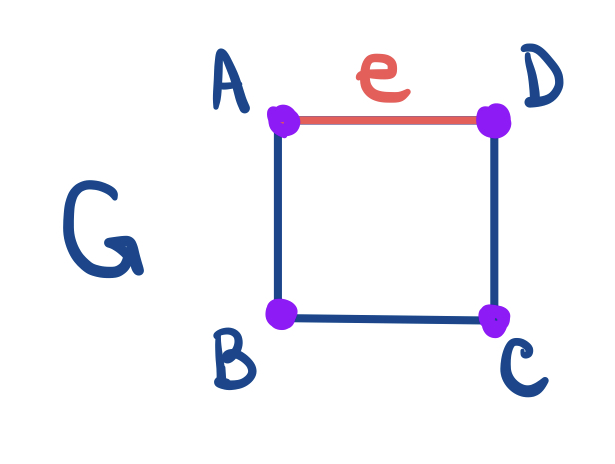
\includegraphics[width=3cm]{pics/coloring_square.jpg}
\end{center}

Its set of vertices is
$$ V = \{ A,B,C,D \}
,$$
and the set of edges is 
$$ E = \{AB,BC,CD,AD\}
.$$

We denote by $e$ the edge $AD$.

Now we can see how we can color this graph using, let's say, 4 colors. We will be coloring the vertices one after another and see which cases we encounter. There are 4 variants for the vertex $A$. For the next vertex, $B$, there are now three variants, because it is connected to one vertex that is already colored. So far, we have $4\cdot 3 = 12$ variants to color two first vertices.

Similarly, after $A$ and $B$ are colored, there are three variants to color $C$. However, we run into trouble now with $D$, because it is connected to both $A$ and $C$, and we don't know if they are the same color or different. Out of the three variants to color $C$, there is one case when $A$ and $C$ are of the same color -- in this case, we can choose out of three colors for $D$; and there are two cases when $A$ and $C$ have different colors -- then in each we can choose out of 2 colors to color $D$. In total, we have the following number of colorings:
$$ P_G(4) = 4 \cdot 3 \cdot (1 \cdot 3 + 2 \cdot 2) = 84
.$$
\end{example}

There is another approach to the same problem where you may choose to ignore the edge $e = AD$. If you delete this edge from $G$, you will get the graph $A_4$, and there we have less restrictions for coloring. In general, when you \emph{delete} $e$ from $G$, the result is denoted by $G-e$.

\begin{center}
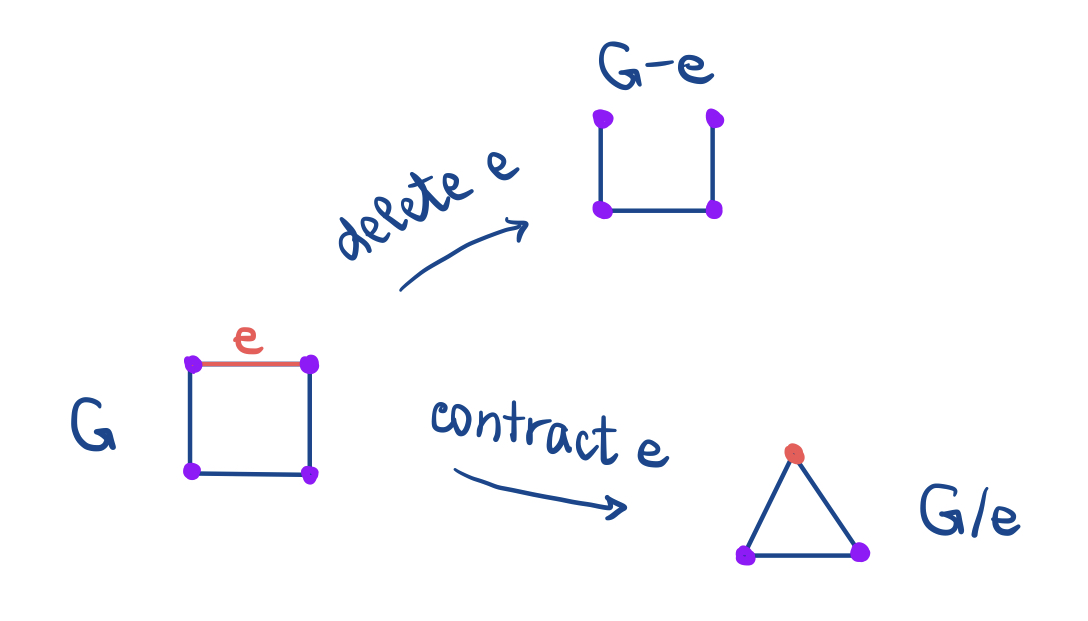
\includegraphics[width=7cm]{pics/coloring_square_deletecontract.jpg}
\end{center}

In fact, for each coloring of $G-e$, there are two cases: 
\begin{enumerate}
    \item Vertices of $e$ (in our case $A$ and $D$) have different colors. In this case, you can restore the edge $e$ and get a coloring of the original graph $G$.
    \item Vertices of $e$ have the same color. Then we can no longer draw an edge between them, because we cannot have an edge that connects vertices of the same color; however, we can glue these two vertices instead. This is called \emph{contracting} the edge $e$ of $G$.
\end{enumerate}

\begin{center}
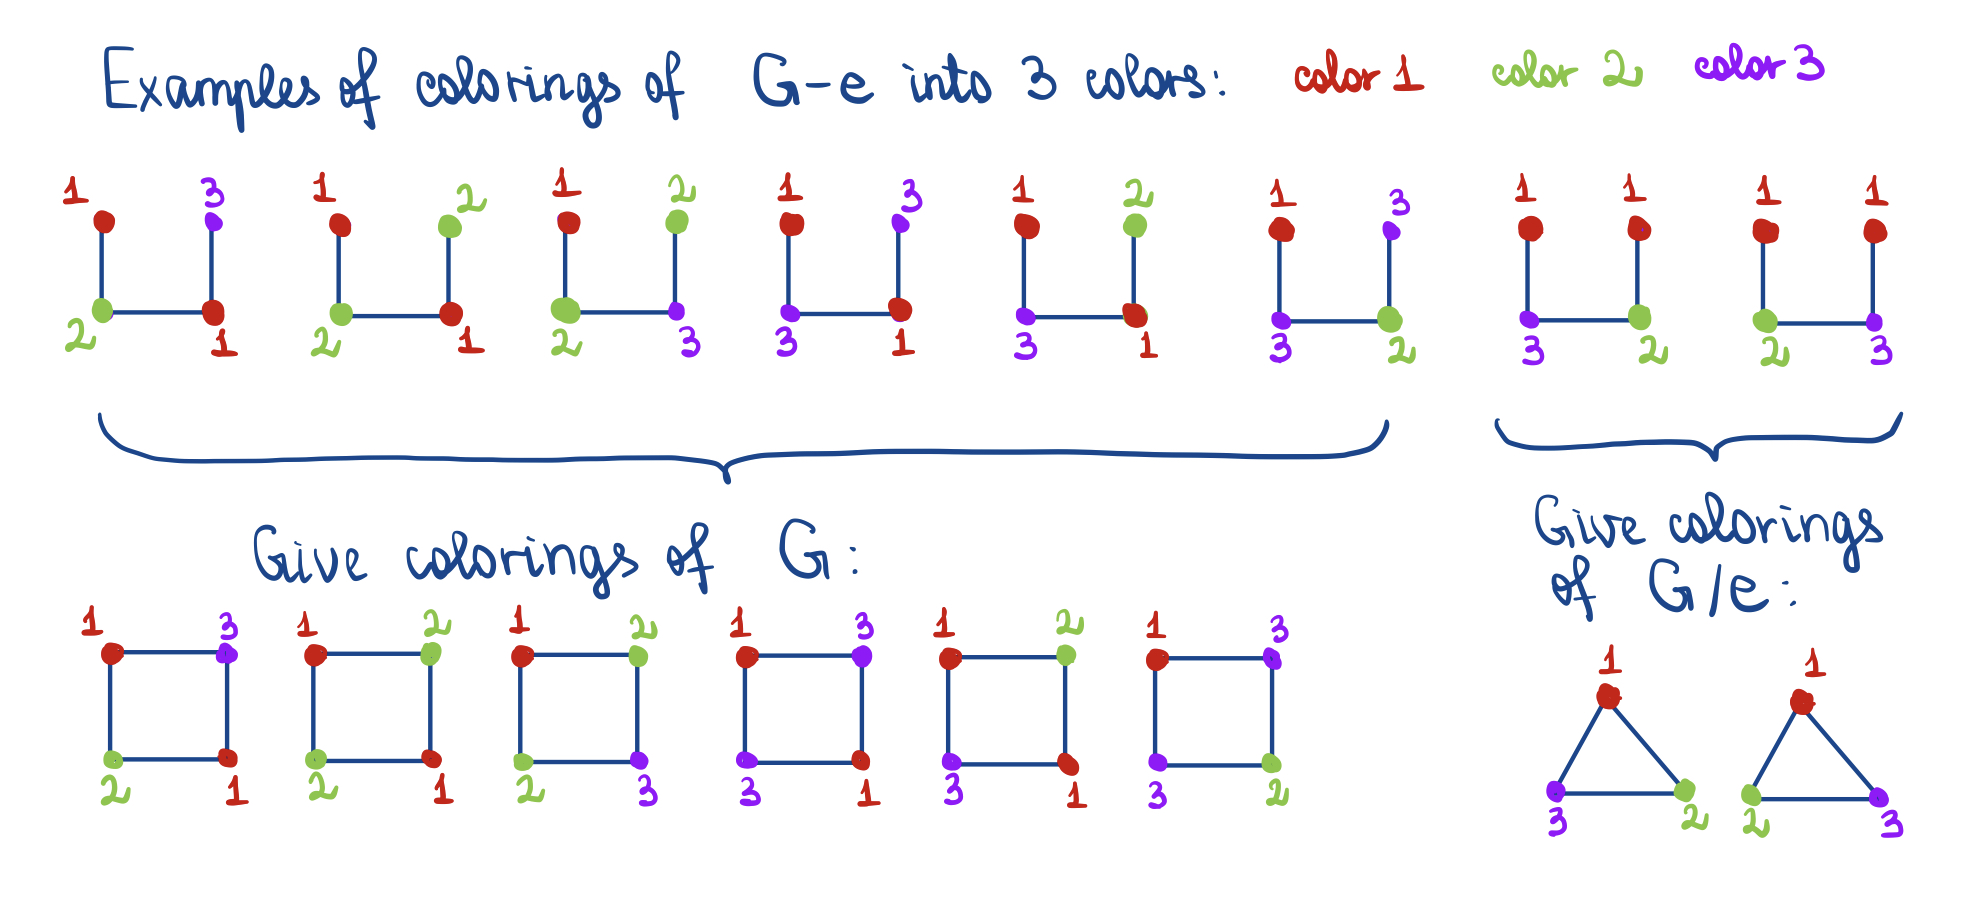
\includegraphics[width=12cm]{pics/coloring_square_cases.jpg}
\end{center}


The following is a cute theorem that generalizes the above observation. To prove it, you may use the same case-by-case analysis as we did for the square, as you may have already noticed that it didn't use the structure of $G$.

\begin{theorem}[Deletion-contraction formula]
   Let $G$ be a graph, and let $G-e$ and $G/e$, respectively, be the graphs obtained 
   from $G$ by deleting and contracting the edge $e$.
   Then
   \begin{equation*}
       P_G(n) = P_{G-e}(n) - P_{G/e}(n)\,.
   \end{equation*}
\end{theorem}

\begin{example}
Returning to the example with the square, denoted again by $G$, we can now compute $P_G(n)$ with the help of the new formula:
$$ P_G(n) = P_{A_4}(n) - P_{G/e}(n) = n(n-1)^3 - P_{G/e}(n)
.$$
Looking at the picture of $G/e$, one can compute $P_{G/e}(n)$: when we first color the vertex $A$, we have $n$ choices; for $B$, since it is connected to $A$, we have $n-1$ choices; and vertex $C$ is connected to $B$ as well as to $A$ (because we contracted $AD$, so $A$ and $D$ are now one vertex) -- so we have $n-2$ choices for $C$, because $A$ and $B$ are two different colors. In total, we have
$$P_{G/e}(n) = n(n-1)(n-2)
$$
colorings of $G/e$.

Finally, we plug in this result into $P_G(n)$:
\begin{equation*}
\begin{split}
    P_G(n) &= n(n-1)^3 - n(n-1)(n-2) = 
n(n-1) \left( (n-1)^2 - (n-2) \right) = \\
    &= n(n-1)(n^2 - 3n +3)
.
\end{split}    
\end{equation*}

We can check that this result recovers our calculation in Example \ref{ex:coloring_square} for $n=4$:
$$ P_G(4) = 4 \cdot 3 \cdot (16 - 12 + 3) = 84
.$$
    
\end{example}




\section{Euler characteristics}

Here is a little bit of magic. 
Close your eyes and start doodling without lifting your pencils.
Don't try too hard because we are going to do some math with your masterpiece.
Here's an example of what a doodling looks like.

\begin{figure}[htpb]
    \centering
    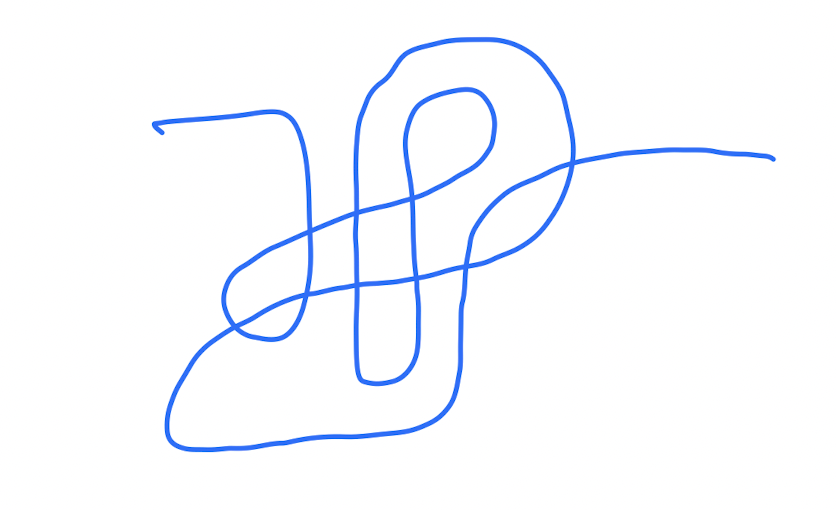
\includegraphics[width=0.4\linewidth]{Figures/doodle1}
    \caption{Doodling}%
    \label{fig:doodle1}
\end{figure}

Now, in order to do some math, please use a red pen to color all the intersections as well as the starting and ending points
in your masterpiece like the Figure~\ref{fig:doodle2}.

\begin{figure}[htpb]
    \centering
    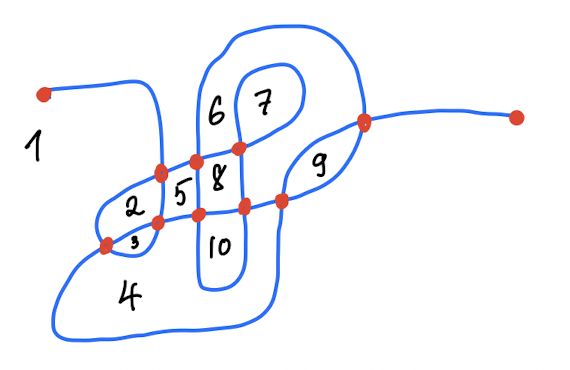
\includegraphics[width=0.4\linewidth]{Figures/doodle2}
    \caption{Color the intersections}%
    \label{fig:doodle2}
\end{figure}

Now, we have turned our doodling into a graph!
Let us count the number of vertices, number of edges and the number of 
regions this graph has divided our paper into (each region is the blank spaced enclosed
by some vertices and edges, just like countries and borders; we also count the area
not enclosed by anything one big region of its own).

Here are the counts for this graph.

\begin{itemize}
    \item Regions: 10
    \item Vertices: 11
    \item Edges: 19
\end{itemize}

Whatever you do, you should have the following relationship:
\begin{equation}
    \label{eq:euler}
    F + V - E = 2 \,,
\end{equation}
where $F$ stands for face (the regions), $V$ stands for vertices, $E$ stands for edges.

\begin{definition}
    The number $\cC(G) = F + V - E$ is called the Euler characteristics of a graph $G$.
\end{definition}

\begin{definition}[Spanning Tree]
   A spanning tree of a graph $G$ is a connected subgraph of $G$ 
   so that every pair of vertices is connected by exactly one path. 
\end{definition}

\begin{proposition}
    \label{t:spanning-tree}
   Every connected graph $G$ contains a spanning tree. 
\end{proposition}
We will not prove this proposition but use it to prove the following theorem.
\begin{theorem}
   The Euler characteristics of a connected planar graph is always 2. 
\end{theorem}

\begin{proof}
    Let $G$ be a connected graph.
    Let $T$ be a spanning tree of $G$ given by Theorem~\ref{t:spanning-tree}.
    For a tree $T$, the number of edges is always one less than the number of vertices, i.e., $V = E + 1$. Because there are no cycles in a tree, the number of faces is $F = 1$.
    So $\cC(T) = 2$. To obtain $G$ from $T$, 
    we add more edges. Each time we add an edge, we add a new face. Thus, the Euler characteristics doesn't change after we add the edges to make $T$ become $G$.
    As a consequence, $\cC(G) = 2$.
\end{proof}


We will have to define what a region means for non-planar graphs (which is out
of the scope of this class) but once we define that, 
we can prove that the Euler characteristics of non-planar graphs are not 2.



Let us use the Euler characteristics to show a very surprising fact about
Platonic solids.

\begin{definition}[Regular polygon]
   A \emph{regular polygon} is a polygon that has all angles equal and all sides equal. 
\end{definition}

\begin{definition}[Platnoic solids]
   A  \emph{Platonic solid} is a 3-dimensional shape such that
   \begin{itemize}
       \item Each face is the same regular polygon.
       \item The same number of polygons meet at each vertex.
   \end{itemize}
\end{definition}

\begin{theorem}
   There are only 5 Platonic solids. 
\end{theorem}

\begin{proof}
    Suppose we have a Platonic solid.
    Let $F$ be the number of faces, $E$ be the number of edges, $V$ be the number
    of vertices of the solid.

    Let us observe a few things.
    First, on each face, the number of edges and vertices is the same.
    Let $N$ be the number of edge and vertices on \emph{each} face. 
    Let $D$ be the degree of each vertex.

    Second, since each edge belongs to two different faces and each 
    edge also joins two vertices,
    \begin{equation*}
        NF = 2E = DV \,.
    \end{equation*}

    Note that we can redraw the faces, vertices and edges of a Platonic solid
    into a plane graph (you should try a few!).
    By the Euler's characteristics theorem,
    \begin{equation*}
        2 = V + F - E   = V + \frac{DV}{N} - \frac{DV}{2} \,. 
    \end{equation*}
    Rearrange terms, we have
    \begin{equation*}
        V(2N + 2D - ND) = 4N \,.
    \end{equation*}
    It must be true then that $2N + 2D - ND > 0$ as $V, N >0$.
    This means $(N- 2)(D-2) <4$ and there are only 5 possibilities for $N, D >0$,

    \begin{equation*}
        (N,D) = \begin{dcases}
            (3,3) \quad \text{ tetrahedron}\,, \\
            (3,4) \quad \text{ cube}\,, \\
            (4,3) \quad \text{ octahedron}\,, \\
            (3,5) \quad \text{ dodecahedron}\,, \\
            (5,3) \quad \text{ icosahedron} \,.
        \end{dcases}
    \end{equation*}
    This is our claim!
\end{proof}




%\chapter{Way after}
%%%
%%%
%\section{Art gallery theorem}
%%%
%\section{Graphs}
%Graphs to describe relations. Chromatic number of a graph. Planar graphs -- start with the game of Brussels Sprouts. Corresponding video: https://www.youtube.com/watch?v=OAss481FfAQ
%%%

%%%
%%%
\chapter{Discrete probability}
%%%
%%%
We will follow the books~\cite{Newstead,DeGroot2012} in this chapter.
Some examples are just copied directly from these books., just as we distinguished the three coins in Example 1.6.3.

We now get to the final chapter of the course.
Probability is perhaps one of the most important concepts in human history.
Since the very ancient time, humans entertain themselves with probability by the
game of chance: gambling... 
This game is almost universal: as far as I can tell, every culture has a version
of gambling that ruins people's lives.
It is very interesting how this game is a universal phenomenon.

At its heart, probability is a little bit paradoxical: it tells us how to predict
randomness! How can one predict anything if everything is random?!
The main point is that probability does not tell you what is going to happen
to one particular sequence of events.
However, it will tell you how likely a sequence of events will happen
with some ``confidence''.
When one uses the language of probability, one needs to be careful not to treat
it as an absolute way to predict something but one needs to allow the possibility 
that the sequence of events under consideration may not happen.


\section{The basics}

In daily language, we talk about the probability of some event to happen 
to mean the following
\begin{equation*}
    \text{Probability of an event happening  }
    = \frac{\text{Number of times the event appear}}{\text{Total number of  outcomes}} \,.
\end{equation*}
Most of the time, we unconsciously think that all the events are equally likely such as the probability for a coin to be head or tail or the probability for a die to be $1,2,\dots, 6$.
This is because we \emph{assume} that there is no reason for the head to appear more often than the tail or $1$ to appear more often than $6$.

\begin{example}
    In daily life, we assume
   \begin{itemize}
       \item The probability for a fair coin to be head is $1/2$.
       \item The probability for a fair die to be 4 is $1/6$.
   \end{itemize} 
\end{example}

However, this assumptioin is not entirely well thought out as there are ways 
to make a coin land on its head more often than its tail.
The coin manufacturer could play with the physics to do it!




\begin{definition}
    Let $A$ be a set.
    The \emph{power set} of $A$, denoted by $\cP(A)$, 
is the set of all subsets of the set $A$. 
\end{definition}

\begin{example}
            $\cP(\set{1,2}) = \set{ \emptyset, \set{1}, \set{2}, \set{1,2}} $.
\end{example}



\begin{definition}
    A \emph{finite discrete probability space} is a pair $(\Omega, \P)$
    where $\Omega$ is a countable set
    and $\P:\cP(\Omega) \to [0,1]$ is a function such that
    \begin{enumerate}
        \item $\P(\Omega) = 1$,
        \item $\P(\bigcup_{i=1}^\infty A_i) = \P(A_1) + \P(A_2) + \dots$ when $A_i\cap A_j = \emptyset$ and $i\not = j$.
    \end{enumerate}
    The set $\Omega$ is called the \emph{sample space}, 
    an element $\omega \in \Omega$ is called an \emph{outcome}, 
    a subset $A \subseteq \Omega$ is called an \emph{event},
    Given $A$, $\P(A)$ is called the \emph{probability of $A$}.
\end{definition}
One can think of the sample space as the set of all possible outcomes. 
An observation based on the above definition is that
a sample space is also an event.

\begin{example}
   Let us model a coin toss.

   The outcomes of the toss are head or tail.
   So, we can take $\Omega = \set{H,T}$.

   The events correspond to the subsets of $\set{H,T}$:
   \begin{enumerate}
       \item $\P(\set{H}) = 1/2 = \P(\set{T})$,
       \item $\P(\emptyset) = 0$,
       \item $\P(\set{H,T}) = 1$.
   \end{enumerate}
\end{example}

\begin{example}
A slightly more interesting thing to talk about is modeling two coin tosses.
In this case, $\Omega = \set{HH, HT, TT,TH}$.
The first letter represents the outcome of the first toss and the second letter the outcome of the second toss.
Here's a few probabilities:
\begin{enumerate}
    \item $\P(\set{HT}) = \P(\set{HH}) = \P(\set{TT})= \P(\set{TT}) = 1/4$
    \item $\P(\set{H}) = \P(\set{HT, HH})  = 1/2$.
\end{enumerate}
\end{example}

\begin{exercise}
    Assume you have a fair coin. Write down the probability space  for three coin tosses.
\end{exercise}

\begin{example}
    Assume you have a fair die. Write down the probability space for one die toss.
    What is the probability for the die to be odd?

    A good way to visualize this is to draw a pie, color the parts that you're looking at and take the area of the colored part and divide it by the total pie.

    \begin{figure}[htpb]
        \centering
        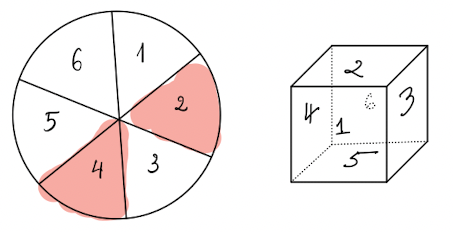
\includegraphics[width=0.8\linewidth]{Figures/pie}
        \caption{The ratio of the color part divided by the total number of equally divided parts gives the probability of the event
        that either the die turns out to be either 2 or 4.}%
        \label{fig:Pie}
    \end{figure}
\end{example}


\begin{proposition}[Some properties of probability]
   The followings are true.
   \begin{enumerate}
       \item $\P(A^C) = 1 - \P(A)$,
       \item $\P(\emptyset) = 0$,
       \item If $A\subseteq B$, then $\P(A) \leq \P(B)$,
       \item $\P(B \cap A^C) = \P(B) - \P(A\cap B)$,
       \item Inclusion-Exclusion principle:
           \begin{equation*}
            \P(A\cup B) = \P(A) + \P(B) - \P(A\cap B) \,.
           \end{equation*}
   \end{enumerate}
\end{proposition}

\begin{proof}
    Let's go through the list.
    \begin{enumerate}
        \item We know that $\Omega = A \cup A^C$ and that $\P(\Omega) = 1$.
            Thus,
            \begin{equation*}
                1 = \P(\Omega) = \P(A) + \P(A^C)\,.
            \end{equation*}
           Rearrange this, we have
           \begin{equation*}
              \P(A^C) = 1 - \P(A) \,. 
           \end{equation*}

       \item $\emptyset = \Omega^C$. Applying (1), we get
           \begin{equation*}
               \P(\emptyset) = 1 - \P(\Omega) = 1-1 = 0 \,.
           \end{equation*}

       \item $B = (B\setminus A) \cup A $. Thus,
           \begin{equation*}
               \P(B) = \P(B \setminus A) + \P(A) \geq \P(A)\,.
           \end{equation*}
           
       \item This follows by the following equation.
           \begin{equation*}
               \P(B) =  \P(B \cap A^C) + \P(B\cap A)\,.
           \end{equation*}
           Rearranging this, we get
           \begin{equation*}
               \P(B\cap A^C) = \P(B) - \P(A\cap B)\,.
           \end{equation*}

       \item We have that 
           \begin{equation*}
               A\cup B = A \cup (B \cap A^C)\,.
           \end{equation*}
           Therefore, using (4),
           \begin{equation*}
            \P(A \cup B) = \P(A) + \P(B \cap A^C) = \P(A) + \P(B) - \P(A \cup B)\,.
           \end{equation*}
    \end{enumerate}
\end{proof}

\begin{example}
   A patient arrives at a doctor’s office with a sore throat and low- grade fever. After an exam, the doctor decides that the patient has either a bacterial infection or a viral infection or both. The doctor decides that there is a probability of 0.7 that the patient has a bacterial infection and a probability of 0.4 that the person has a viral infection. What is the probability that the patient has both infections? 
\end{example}

\begin{example}
    Inherited traits in humans are determined by material in specific locations
on chromosomes. Each normal human receives 23 chromosomes from each parent,
and these chromosomes are naturally paired, with one chromosome in each pair coming from each parent. For the purposes of this text, it is safe to think of a gene as a portion of each chromosome in a pair. The genes, either one at a time or in combination, determine the inherited traits, such as blood type and hair color. The material in the two locations that make up a gene on the pair of chromosomes comes in forms called alleles. Each distinct combination of alleles (one on each chromosome) is called a genotype.

Consider a gene with only two different alleles A and a. Suppose that both parents have genotype Aa, that is, each parent has allele A on one chromosome and allele a on the other. (We do not distinguish the same alleles in a different order as a different genotype. For example, aA would be the same genotype as Aa. But it can be convenient to distinguish the two chromosomes during intermediate steps in probability calculations.) What are the possible genotypes of an offspring of these two parents? If all possible results of the parents contributing pairs of alleles are equally likely, what are the probabilities of the different genotypes? 
\end{example}


\section{Probability from counting }
Let us learn how to come up with probability law for 
some``simple'' situations, where the number of outcomes is finite. 
We call this finite probability (as opposed to countably inifinite probability).
We will assume that every outcome is equally likely to another
and, hence, in order to determine the probability of an event, one needs to be
able to count accurately.
The general principle is
\begin{equation}
    \label{eq:gen-principle}
    \text{Probability of an event happening  }
    = \frac{\text{Number of ways it can appear}}{\text{Total number of  outcomes}} \,.
\end{equation}

\begin{example}
    Let $A_3$ be the graph in homework 8.
    Suppose we have 4 colors: red, blue, yellow, green.
    Assume that each coloring is equally likely. Write down 
    the probability space for the chance for a particular way of coloring is chosen.
\end{example}

\begin{example}
    Let $K_3$ be the complete graph with 3 vertices.
    Suppose we have 4 colors: red, blue, yellow, green.
    Assume that each coloring is equally likely. Write down 
    the probability space for the chance for a particular way of coloring is chosen.
\end{example}
Thus, it is important to learn how to count.

\subsection{Counting}
In order to apply the general principle~\ref{eq:gen-principle}, we need to know
the total number of outcomes.
One could list them all out. However, when the number of outcomes gets large,
this is very inefficient and often leads to errors.
It is nice to have a way (formula) to find the total number of outcomes efficiently.
This section will discuss several ways, which we can use to do just that.


\begin{example}
   Consider an experiment that has the following two characteristics: 
    \begin{enumerate}
        \item The experiment is performed in two parts.
        \item The first part has $m$ possible outcomes and regardless
            of which outcome in part 1 we end up with, the second part
            always has $n$ possible outcomes.
    \end{enumerate}
    How many possible outcomes can one have?
    Find a way to write down the sample space in mathematical langauge.
\end{example}

One can show the following general theorem using induction.
\begin{theorem}[Multiplication rule]
    Suppose that an experiment has k parts $(k\geq 2)$, that the $i^{th}$ part of the experiment can have 
    $n_i$ possible outcomes $(i = 1,..., k)$, and that all of the outcomes in 
    each part can occur regardless of which specific outcomes have occurred in the other parts.
    Then the sample space $\Omega$ will have $n_1n_2\dots n_k$ outcomes.
\end{theorem}

In the above theorem, it is assumed that the number of outcomes in each part of the experiment 
does not depend on that of the other parts.
This is not the case in general as one might imagine that when one does a survey,
one does not ask the same person to fill out the survey multiple times.
This process is called \emph{sampling without replacement}.

\begin{example}
    \label{ex:n-permute-3}
   Consider an experiment in which a card is selected and removed from a deck of n different cards, a second card is then selected and removed from the remaining $n -1$ cards, and finally a third card is selected from the remaining $n- 2$ cards. Each outcome consists of the three cards in the order selected. A process of this kind is called sampling without replacement, since a card that is drawn is not replaced in the deck before the next card is selected. In this experiment, any one of the n cards could be selected first. Once this card has been removed, any one of the other $n-1$ cards could be selected second. Therefore, there are $n(n-1)$
    possible outcomes for the first two selections. Finally, for every given outcome of the first two selections, there are $n-2$ other cards that could possibly be selected third. Therefore, the total number of possible outcomes for all three selections is $n(n-1)(n-2)$.
\end{example}


\begin{definition}[Permutation]
Suppose that a set has $n$ elements. Suppose that an experiment consists  
of selecting $k$ of the elements one at a time without replacement. 
Let each outcome consist of the $k$ elements in the order selected. 
Each such outcome is called a \emph{permutation} of $n$ elements taken $k$ at a time. 
We denote the number of distinct such
permutations by the symbol $P_{n,k}$.

We say ``$n$ permute $k$'' to talk about $P_{n,k}$.
\end{definition}

\begin{example}
    We see from the Example~\ref{ex:n-permute-3} that $n$ permute $3$ is
    $P_{n,3} = n(n-1)(n-2)$.
    An astute observer would see that
    \begin{equation*}
        P_{n,n} = n(n-1)(n-2)\cdot...\cdot 2\cdot 1  \,.
    \end{equation*}
\end{example}

\begin{definition}[Factorial]
    We write $n! = n(n-1)\cdot \dots \cdot 2 \cdot 1$ and call it ``$n$ factorial''.
    Thus, 
    \begin{equation*}
        n! \defeq P_{n,n} \,.
    \end{equation*}
\end{definition}

\begin{example}
    From the above definition, $0! = 1$ as there is one way to order an empty set 
    -- you don't do anything!
   We have that for $n \geq k \geq 0$,
   \begin{equation*}
       P_{n,k} = \frac{n!}{k!} \,.
   \end{equation*}
\end{example}

Another way to think about permutation is the way of 
selecting (without replacement) $k$ out of $n$ elements where the order of the elements matter.
Sometimes, one does NOT care about the order of the selection. 
This leads to the concept of \emph{combination}.

\begin{definition}
    Consider a set of $n$ elements. Each subset of size $k$ chosen from this set
    is called a \emph{combination of $n$ elements taken $k$ at a time}.
    We denote the number of distinct such combinations by the symbol
    $C_{n,k}$, or often enough $\binom nk$.
\end{definition}

\begin{theorem}
    For $n\geq k \geq 0$, we have that
   \begin{equation*}
       C_{n,k} = \frac{P_{n,k}}{k!} = \frac{n!}{k!(n-k)!} \,.
   \end{equation*}
\end{theorem}

\begin{theorem}[Binomial theorem]
    For all numbers $x$ and $y$,
    \begin{equation*}
        (x+y)^n = \sum_{k=0}^n \binom nk x^{k}y^{n-k} \,.
    \end{equation*}
    Because of this formula, $\binom nk$ is often referred to as a 
    \emph{binomial coefficient}.
\end{theorem}

\begin{example}
    \label{ex:blood}
   The gene for human blood type consists of a pair of alleles chosen from
   the three alleles commonly called $O, A$ and $B$.
   For example, a possible combination of alleles is $AA$.
   There is no distiction between the orders of the combination, $OA$ would
   be the same with $AO$.
   There are $3$ pairs where both alleles are the same and
   $\binom 32$ pairs where the alleles are different.
   Thus, the number of possible blood type is
   \begin{equation*}
       3 + \binom 32 = 3 + \frac{3!}{2!}{1!} = 3+ 3 = 6\,.
   \end{equation*}
   Can you think of another way to derrive this number?
\end{example}

\begin{question}
    What happen if there is an alien that has $n$ alleles but the blood type 
    is still the combination of the alleles? How many possible blood type does
    this alien have?
\end{question}

\subsection{Generating probability from counting}
Recall the principle
\begin{equation*}
    \text{Probability of an event happening  }
    = \frac{\text{Number of ways it can appear}}{\text{Total number of  outcomes}} \,.
\end{equation*}
We will have some examples to get used to using this to find out the probability 
of something happening.

\begin{example}
    Suppose a fair coin is tossed 10 times.
    What is the probability that
    \begin{enumerate}
        \item exactly 3 heads appear.
        \item 3 or fewer heads appear.
    \end{enumerate}

    In total, there are $2^{10}$ possibilities.

    \begin{enumerate}
        \item The number of ways three heads can appear is $\binom {10}3$.
            So the probability for exactly 3 heads to appear is
            \begin{equation*}
                \frac{\binom {10}3}{2^{10}} = 0.1172 \,.
            \end{equation*}

        \item The number of ways three or fewer heads appear would be the sum
            of the numbers of ways exactly $0, 1,2$ or $3$ heads appear
            \begin{equation*}
                \binom {10}0 + \binom {10}1 + \binom {10}2 + \binom {10}3 \,.
            \end{equation*}
            Thus, the probability for three or fewer heads to appear is
            \begin{equation*}
                \frac{ \binom {10}0 + \binom {10}1 + \binom {10}2 + \binom {10}3 }{ 2^{10}} = 0.1719 \,.
            \end{equation*}
    \end{enumerate}
\end{example}


\begin{example}
   Suppose a class contains 15 men and 30 women and that 10 students are selected
   at random with equal probability.
   What is the probability that exactly 3 men are selected?

   There are $\binom {45}{10}$ ways to select 10 students out of 45.

   Because there are three men to be selected, there are seven women that would
   be selected. The number of ways for this to happen is
    \begin{equation*}
        \binom {15}{3} \binom{30}7 \,.
    \end{equation*}
    So the probability to select exactly three men out of the 45 students is
    \begin{equation*}
        \frac{ \binom {15}{3} \binom{30}7}{ \binom {45}{10}} = 0.2904 \,. 
    \end{equation*}
\end{example}

\begin{example}
    There is a deck of 52 cards that have been shuffled thoroughly.
    There are four players and each player receives 13 cards.
    What is the probability that each player receives exactly one ace?

    If each player were to receive one ace, there are $13^4$ possible positions
    that the aces could appear.

    Without this restriction that each player were to receive one ace,
    there are $\binom {52}4$ positions that the aces could appear.
    \begin{equation*}
        \frac{13^4}{\binom {52}4} = 0.1055 \,.
    \end{equation*}
\end{example}

\section{Conditional probability}
The idea of probability is based on the likelihood of something to happen
within an idealized universe.
Say, within the universe of MATH 170,  $50\%$ of the students is female.
However, if one expand the universe to the entire human population on earth,
according to the Worldbank, the number is $49.585\%$.
This opens up the idea of conditional probability, where we ``zoom'' into one universe to study the odds of certain events to happen without worrying about
the odds of the same events to happen in the bigger universe.


\begin{definition}[Conditional probability]
    Given a probability space $(\Omega, \P)$ and events $A$ and $B$.
    \emph{The conditional probability of the event $A$ given that the event $B$
        has occured}, denoted by $\P(A\st B)$, is given by
        \begin{equation*}
            \P(A\st B) \defeq \frac{\P(A\cap B)}{\P(B)} \,.
        \end{equation*}
        Typically, we read the above as ``probability of $A$ given $B$''.
\end{definition}

It is sometimes good to draw the Venn diagram to see what's going on with
probability.
\begin{example}
    Consider the following figure
    \begin{figure}[h]
        \centering
        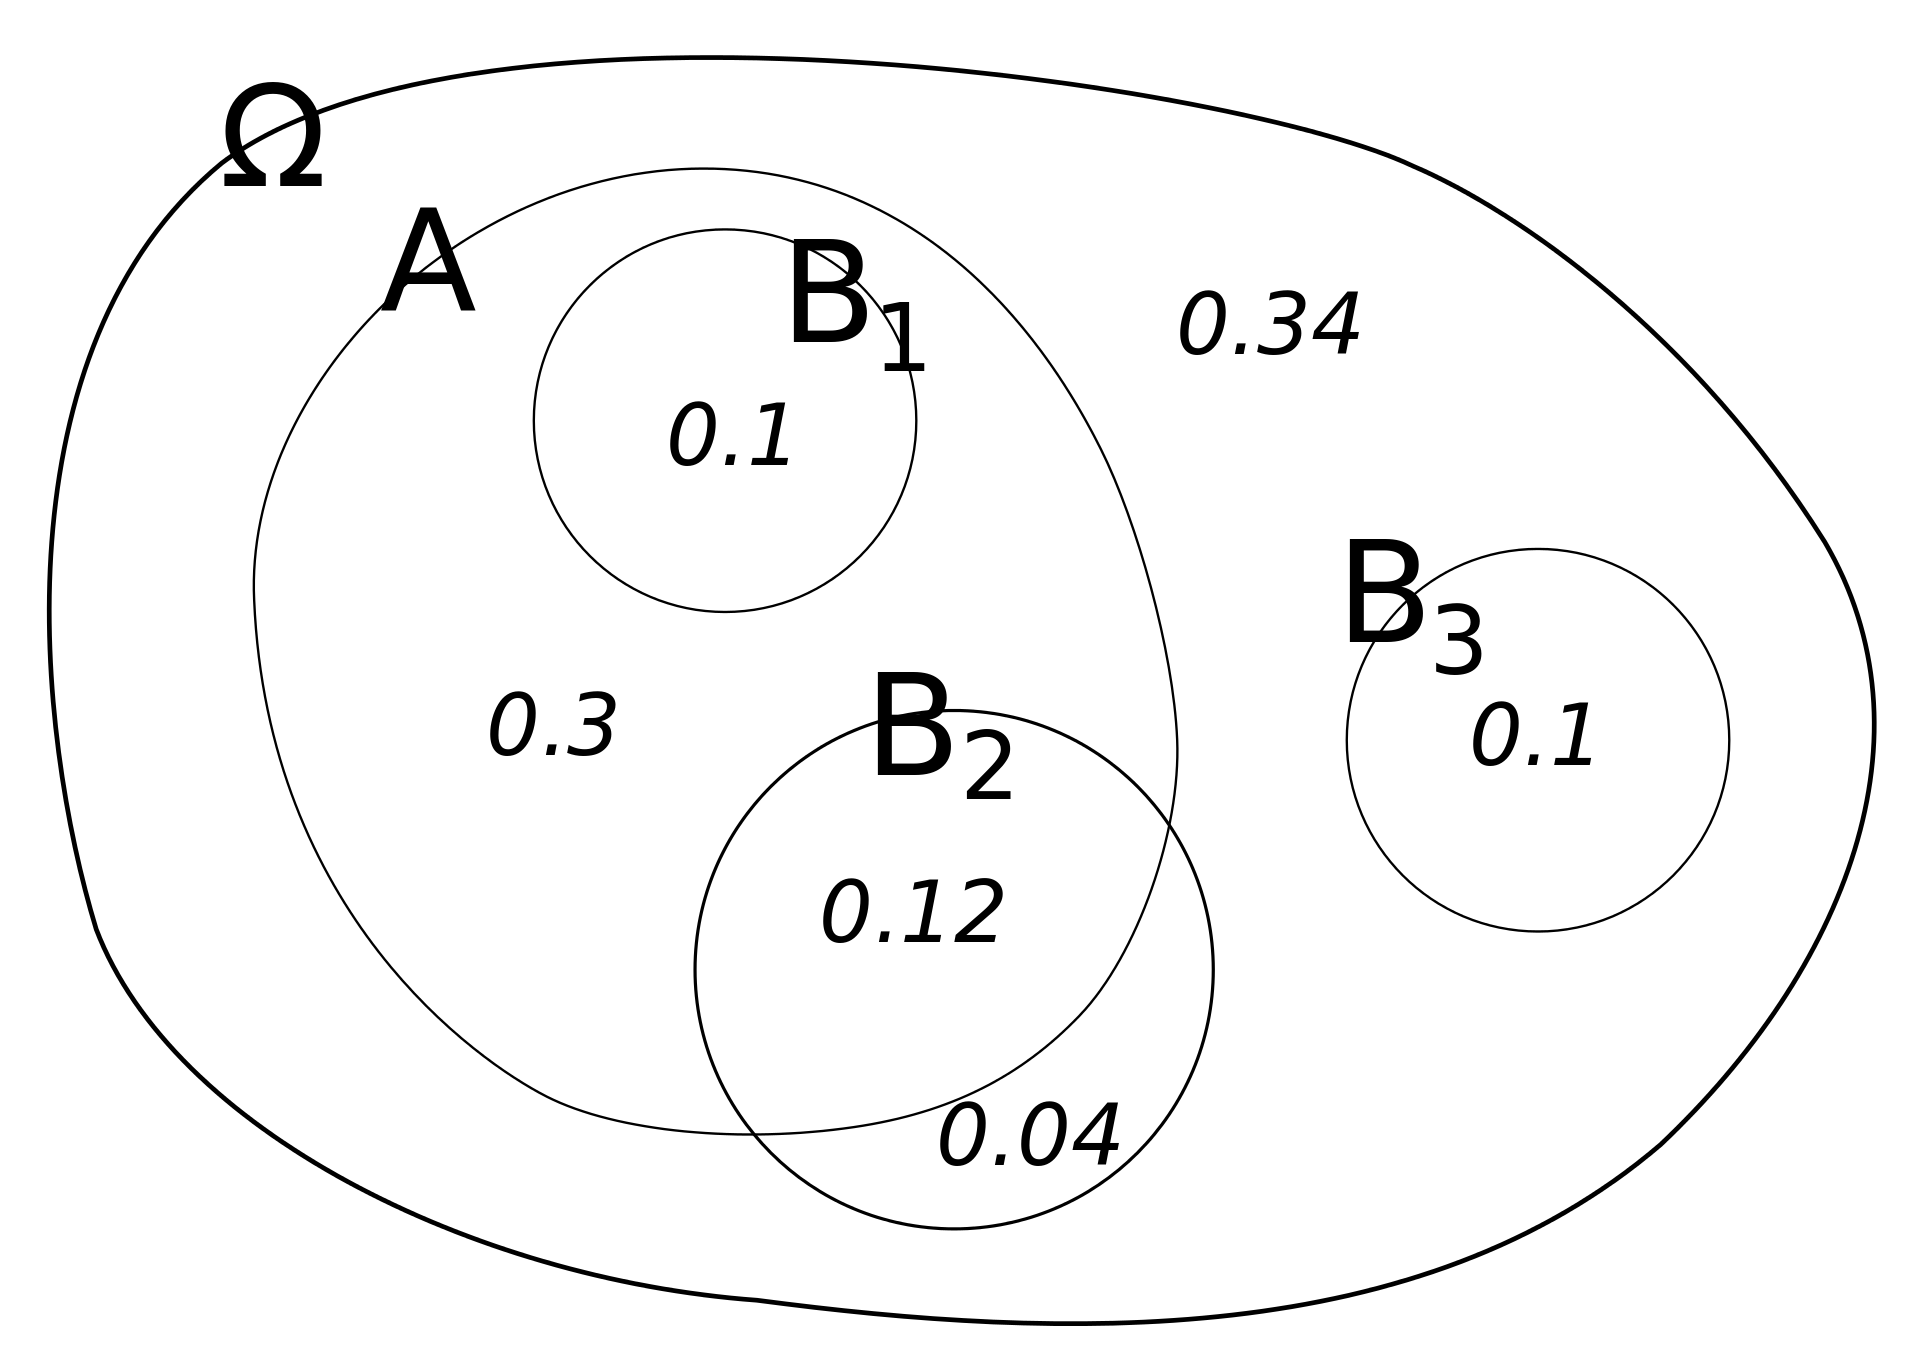
\includegraphics[width=0.4\linewidth]{Figures/Conditional_probability}
        \caption{Sets in $\Omega$ (from Wikipedia)}%
        \label{fig:conditional-prob}
    \end{figure}
    The unconditional probability $\P(A) = 0.30 + 0.10 + 0.12 = 0.52$. 
    However, the conditional probability 
    $P(A\st B_1) = 1$, 
    $P(A\st B_2) = 0.12 ÷ (0.12 + 0.04) = 0.75$, 
    and $P(A\st B_3) = 0$.
\end{example}



\begin{example}
   Here's something from Wikipedia.
   Even if 100\% of patients with pancreatic cancer have a certain symptom, when someone has the same symptom, it does not mean that this person has a 100\% 
   chance of getting pancreatic cancer. Assume the incidence rate of pancreatic cancer is 1/100000, 
   while 10/100000 healthy individuals have the same symptoms worldwide, 
   the probability of having pancreatic cancer given the symptoms is only 9.1\%, 
   and the other 90.9\% could be "false positives" (that is, falsely said to have 
   cancer; "positive" is a confusing term when, as here, the test gives bad news).
    Based on incidence rate, the following table presents the corresponding numbers per 100,000 people.
   \begin{figure}[h]
       \centering
       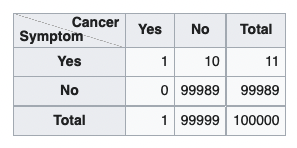
\includegraphics[width=0.4\linewidth]{Figures/cancer}
       \label{fig:cancer}
   \end{figure} 

   Which can then be used to calculate the probability of having cancer when you have the symptoms:
   \begin{align*}
&P(\text{Cancer}|\text{Symptoms})\\ &= \frac{P(\text{Symptoms}|\text{Cancer}) P(\text{Cancer})}{P(\text{Symptoms})} \\
 &= \frac{P(\text{Symptoms}|\text{Cancer}) P(\text{Cancer})}{P(\text{Symptoms}|\text{Cancer}) P(\text{Cancer}) + P(\text{Symptoms}|\text{Non-Cancer}) P(\text{Non-Cancer})} \\[8pt]
&= \frac{1 \times 0.00001}{1 \times 0.00001 + (10/99999) \times 0.99999} = \frac1{11} \approx 9.1\%
\end{align*}
\end{example}

\section{Independence}

\begin{example}
  Suppose that a fair coin is tossed twice. 
  The experiment has four outcomes, 
  $HH, HT, TH$, and $TT$, that tell us how the coin landed on each of the two tosses. 
  We can assume that this sample space is simple so that each 
  outcome has probability $1/4$. 
  Suppose that we are interested in the second toss. 
  In particular, we want to calculate the probability of the event 
  $A = \{ H \text{ on second toss}\}$. 
  We see that $A = \{HH,TH \}$, 
  so that $\P(A) = 2/4 = 1/2$. 
  If we learn that the first coin landed $T$, 
  we might wish to compute the conditional probability 
  $\P(A|B)$ where 
  $B = \{T  \text{ on first toss} \}$. 
  Using the definition of conditional probability, we easily compute  
  \begin{equation*}
      \P(A\st B) = \frac{\P(A\cap B)}{\P(B)} = \frac{1/4}{1/2} = \frac{1}{2} = \P(A) \,.
  \end{equation*}
  So, we can see that
  \begin{equation*}
      \P(A\cap B) = \P(A) \P(B) \,.
  \end{equation*}
    Another way to view this is that 
    $A$ doesn't live under the world of $B$. 
    What happens to $B$ doesn NOT affect what happens in $A$.
\end{example}

This inspires the following definition.
\begin{definition}[Independence]
   Two events $A$ and $B$ are independent if
   \begin{equation*}
       \P(A\cap B) = \P(A)\P(B)\,.
   \end{equation*}
\end{definition}

The example with the coin does not seem to have any consequence in our daily life.
However, understanding probability (or anything) could mean life or death.
There are a lot of tragedies when people misuse probability and deduce wrong conclusions
that lead to deaths of others.

\begin{example}
    In this example, we will write SIDS for Sudden Infant Death Syndrome.
    Sally Clark\footnote{\url{https://en.wikipedia.org/wiki/Sally_Clark}\\ \url{https://blogs.cornell.edu/info2040/2018/11/28/bayes-theorem-in-the-court-the-prosecutors-fallacy/}} (1964-2007) was an English woman who was wrongly accused of
    murdering her own children in 1999. 
    In the trial, certain ``expert'' Roy Meadow, calculated the following probaility:
    \begin{enumerate}
        \item $\P(\text{1 SIDS in a relatively well-off family}) \approx 1/8500$,
        \item $\P(\text{2 SIDS in a relatively well-off family}) \approx  (1/8500)^2 = 1/73 \text{million}$.
    \end{enumerate}
    From this, he concluded that this event happens once in 100 years and it is likely that Sally was guilty of killing her own children.
    The court ruled accordingly.
    This is WRONG! For a few reasons.

    \begin{enumerate}
        \item You need to look at the probability of SIDS in a typical family, not a well-off family.
            This probability turns out to be $1/1300$.
        \item Two SIDS in the same family are not two independent events.
        \item A chance for a mother to kill her own baby is \emph{incredibly low}.
    \end{enumerate}
    Let's do a conservative calculation to see the lowest chance for Sally Clark to be guilty, given the evidence provided in court.
    The key words here are ``given the evidence''.

    Let us have a few statistics up.
    Let us set up some notations.
    \begin{enumerate}
        \item $\P(\text{1 SIDS }) \approx 1/1,300$,
        \item $\P(\text{SIDS in a  family given there's already 1 SIDS}) \approx 1/130$,
        \item $\P( \text{ two children in the same household dies not from SIDS}) \approx 3/650,000$.
    \end{enumerate}

    So, from (1) and (2) already, we have
    \begin{equation*}
        \P(\text{2 SIDS in a  family}) \approx \frac{1}{1300}\frac{1}{130} = \frac{1}{169,000}\,.
    \end{equation*}
    This is still about 1/1million.
    But this still doesn't tell us about the chance that Clark murderred her children.
    Let us use the knowledge of conditional probability to proceed.
    Let $D$ denote the event of two death babies, $H$ be the event of 2 SIDS in a family, 
    Note that $H \subseteq D$. Therefore,
    \begin{align*}
        \P( H \st D) &  
        = \frac{ \P(H \cap D)  }{ \P(D)  } 
                     = \frac{ \P(H)  }{ \P(D\cap H) + \P( D \cap H^C)  } 
                     = \frac{ \P(H)  }{ \P(H) + \P(   D \st H^C) \P(H^C)   } \\
                     &\approx \frac{ 1/169,000}{ 1/169,000 + (1 - 1/169,000)* 3/650,000  } \approx 0.56\,.
    \end{align*}
    There is more chance for Sally Clark to not kill both babies than to kill. 
    This is, of course, not enough to overturn the juridiction but it is not a 
    death sentence as the previous outrageous calculation. 
\end{example}

Denote the notation
\begin{equation*}
    \sum_{i=1}^k a_i \defeq a_1 + \dots + a_k\,.
\end{equation*}

\begin{theorem}[Bayes Theorem]
    Let $(\Omega,\P)$ be a probability space.
    Let $B_1, \dots, B_k$ be disjoint events such that 
    $\P(B_i) > 0$ for $i= 1, \dots, k$ and
    \begin{equation*}
        B_1 \cup B_2 \cup \dots \cup B_k = \Omega\,.
    \end{equation*}
    Then
   \begin{equation*}
       \P(B_i\st A) = \frac{ \P(B_i\cap A) }{ \sum_{i = 1}^k \P(B_i)\P(A\st B_i)} \,.
   \end{equation*} 
\end{theorem}

\section{Random Variable and Expectation}

\begin{definition}
   Given a sample space $\Omega$. A discrete random variable $X$ is a function 
   $X:\Omega \to \N$.
\end{definition}

With this definition, we can ask what is the likelihood of $X = 1$?
Denote 
$\set{X = n}$ the event that consists of all the outcomes $\omega\in \Omega$ so that $X(\omega) = n$.

So,
\begin{equation*}
    \set{X=n} \defeq \set{ \omega \in \Omega \st X(\omega) = n}\,.
\end{equation*}
We can certainly compute 
\begin{equation*}
    \P(\set{X = n})
\end{equation*}
if we know the probability function $\P$.

\begin{definition}[Expectation]
   Let $(\Omega, \P)$ be a probability space and $X$ be a discrete random variable.
   Let $p_n = \P({X= n})$.
   The \emph{expectation} of $X$ is defined by
   \begin{equation*}
       \E(X) \defeq \sum_{n= 0}^\infty n p_n \,.
   \end{equation*}
   Sometimes we use $\mu$ to be the notation for $\E(X)$.
\end{definition}

\begin{definition}[Standard deviation]
   The \emph{variance} of $X$ is defined by 
   \begin{equation*}
      Var(X) \defeq \E( (X-\mu)^2)=   \sum_{n=0}^\infty (n - \mu)^2 p_n\,.  
   \end{equation*}
    The \emph{standard deviation} of $X$ is
    \begin{equation*}
        \sigma_X = \sqrt{Var(X)}\,.
    \end{equation*}
        
\end{definition}






\printbibliography 
%\bibliography{refs}
%\bibliographystyle{halpha-abbrv}


\end{document}
